\documentclass[cmfont,usenames,dvipsnames,leqno]{afit-etd}\usepackage[]{graphicx}\usepackage[]{color}
%% maxwidth is the original width if it is less than linewidth
%% otherwise use linewidth (to make sure the graphics do not exceed the margin)
\makeatletter
\def\maxwidth{ %
  \ifdim\Gin@nat@width>\linewidth
    \linewidth
  \else
    \Gin@nat@width
  \fi
}
\makeatother

\definecolor{fgcolor}{rgb}{0.345, 0.345, 0.345}
\newcommand{\hlnum}[1]{\textcolor[rgb]{0.686,0.059,0.569}{#1}}%
\newcommand{\hlstr}[1]{\textcolor[rgb]{0.192,0.494,0.8}{#1}}%
\newcommand{\hlcom}[1]{\textcolor[rgb]{0.678,0.584,0.686}{\textit{#1}}}%
\newcommand{\hlopt}[1]{\textcolor[rgb]{0,0,0}{#1}}%
\newcommand{\hlstd}[1]{\textcolor[rgb]{0.345,0.345,0.345}{#1}}%
\newcommand{\hlkwa}[1]{\textcolor[rgb]{0.161,0.373,0.58}{\textbf{#1}}}%
\newcommand{\hlkwb}[1]{\textcolor[rgb]{0.69,0.353,0.396}{#1}}%
\newcommand{\hlkwc}[1]{\textcolor[rgb]{0.333,0.667,0.333}{#1}}%
\newcommand{\hlkwd}[1]{\textcolor[rgb]{0.737,0.353,0.396}{\textbf{#1}}}%

\usepackage{framed}
\makeatletter
\newenvironment{kframe}{%
 \def\at@end@of@kframe{}%
 \ifinner\ifhmode%
  \def\at@end@of@kframe{\end{minipage}}%
  \begin{minipage}{\columnwidth}%
 \fi\fi%
 \def\FrameCommand##1{\hskip\@totalleftmargin \hskip-\fboxsep
 \colorbox{shadecolor}{##1}\hskip-\fboxsep
     % There is no \\@totalrightmargin, so:
     \hskip-\linewidth \hskip-\@totalleftmargin \hskip\columnwidth}%
 \MakeFramed {\advance\hsize-\width
   \@totalleftmargin\z@ \linewidth\hsize
   \@setminipage}}%
 {\par\unskip\endMakeFramed%
 \at@end@of@kframe}
\makeatother

\definecolor{shadecolor}{rgb}{.97, .97, .97}
\definecolor{messagecolor}{rgb}{0, 0, 0}
\definecolor{warningcolor}{rgb}{1, 0, 1}
\definecolor{errorcolor}{rgb}{1, 0, 0}
\newenvironment{knitrout}{}{} % an empty environment to be redefined in TeX

\usepackage{alltt}

% The afit-etd class requires the following packages: url, refcount, graphicx,
%                                                     sf298, hyperref
%
% Required files to support the afit-etd class are:
%      afit-etd.cls
%      afitlogo.pdf or afitlogo.eps
%      af298.sty (slight modifications implemented to fix a 'glitch')
%
% All of the required files must be located in your LaTeX search path.  The
% easiest place to put them is in the working directory along with this
% thesis.tex file.


% Additional files used in this shell but not required are:
%     thesis.bib (used as an example only)
%     thesnum3.bst (can be replaced with any other bibliography style file)
%     CampusPhoto.pdf and CampusPhoto.eps (used as an example only)
%
% This shell will not process without these files, but if you delete sample
% text and replace the BST file with another, then these will not be required
% at all.


% Options for the afit-etd class are: 
%      cmfont    - revert to TeX's computer modern font (Times New Roman is the
%                  default) 
%      11pt      - use an 11 pt font instead of the default 12 pt font
%      nonumbers - employ a format, as shown in the AFIT style guide, that
%                  omits the section numbers for all headings except chapters
%      draft     - draws frames where graphics would be instead of actually
%                  including graphics.  This is a standard LaTeX option and
%                  will have other effects based on the packages used

% Send bug reports to the author at: Michael.Stepaniak@us.af.mil

% The following packages and macros are recommended but not required:
\usepackage{mathtools,graphicx,enumerate,float,booktabs,url,amsthm,framed,bm,amsfonts,acronym,mathrsfs}
\usepackage[boxed, ruled]{algorithm2e}
% \usepackage[printonlyused]{acronym}  
\usepackage[round]{natbib}
%\usepackage[square,sort&compress,numbers]{natbib} % better citations especially
                                                   % when including a string of 
                                                   % citations

%% Change hyperlink options
\hypersetup{
  colorlinks=true, % false: boxed links; true: colored links
  linkcolor=blue,   % color of internal links (change box color with linkbordercolor)
  citecolor=blue, % color of links to bibliography
  urlcolor=blue    % color of external links
}

%% Make sure line spacing isn't changed in knitr output
\renewenvironment{knitrout}{\begin{singlespace}}{\end{singlespace}}

%% Define R example environment
\newtheorem{rexample}{R Example}[section]

%% Define new commands
\newcommand{\newln}{\\&\quad\quad\quad\quad{}}
\newcommand{\loglik}{\mathscr{L}}
\newcommand{\boot}{\star} % or possiibly *
\newcommand{\indep}{\perp \! \! \! \perp} 
\newcommand{\code}[1]{\texttt{\small{#1}}}
\newcommand{\pkg}[1]{\textsf{\small{#1}}}
\newcommand{\norm}[1]{\left\|#1\right\|}
\newcommand{\trans}{\ensuremath{^\prime}}
\newcommand{\bc}[1]{\ensuremath{\bm{\mathcal{#1}}}}
\newcommand{\mc}[1]{\ensuremath{\mathcal{#1}}}
\newcommand{\wh}[1]{\ensuremath{\widehat{#1}}}
\newcommand{\wt}[1]{\ensuremath{\widetilde{#1}}}
\newcommand{\wb}[1]{\ensuremath{\overline{#1}}}
\newcommand{\tquant}[2]{\ensuremath{t_{#1,#2}}}

%% Define new operators
\newcommand{\argmin}[1]{\underset{#1}{\operatorname{arg}\!\operatorname{min}}\;}
\newcommand{\E}{\operatorname{E}}
\newcommand{\var}{\operatorname{Var}}
\newcommand{\cov}{\operatorname{Cov}}
\newcommand{\se}{\operatorname{se}}
\newcommand{\diag}{\operatorname{diag}}
\newcommand{\bias}{\operatorname{Bias}}
\newcommand{\MSE}{\operatorname{MSE}}
\newcommand{\PSS}{\operatorname{PSS}}
\newcommand{\tr}{\operatorname{tr}}
\newcommand{\X}{\ensuremath{\bm{X}}}
\newcommand{\Z}{\ensuremath{\bm{Z}}}
\newcommand{\Prob}{\operatorname{Pr}}
\newcommand{\RSS}{\operatorname{RSS}}

%\allowdisplaybreaks

%% Required front matter definitions -------------------------------------------

%\title  {A \LaTeX{} Template for AFIT Theses, Dissertations,\\
%         and Graduate Research Papers} % \\ can be used to force a linebreak
\title{Topics in Statistical Calibration}
\doctype{DISSERTATION} % or GRADUATE RESEARCH PAPER, DISSERTATION, or REPORT PROSPECTUS
                 % REPORT will generate a simplified format more suitable for
                 % class assignments

\author          {Brandon M.}{Greenwell}
\rank            {Civilian}
\previousdegrees {B.S., M.S.} % Abbreviate any previous degrees

% Uncomment the following lines if there is a second author
% \coauthor          {FirstName I. LastName} 
% \corank            {Major, USAF}
% \copreviousdegrees {B.S.} 

\degree          {Doctor of Philosophy}
\graduation      {27}{March}{2014} % format is {DD}{Month}{YYYY} where
                                   % Month must be: March, June,
                                   % September, or December

\designator{AFIT-ENC-DS-14-M-01} % assigned by the graduate advisor in
                               % during the student's final quarter


\distribution{DISTRIBUTION STATEMENT A:\\APPROVED FOR PUBLIC RELEASE;
  DISTRIBUTION UNLIMITED} % or other appropriate distribution statement from the
                          % AFIT Style Guide

\committee{ % Advisor must be listed first in the list of committee members
  {Christine M. Schubert Kabban, PhD (Chairman)},
  {Raymond Hill, PhD (Member)},
  {Dursun Bulutoglu, PhD (Member)}
}

\department {Department of Mathematics and Statistics}
\school     {Graduate School of Engineering and Management}
\dean       {ADEDEJI B. BADIRU{,} PhD} % only used for PhD dissertations

% Uncomment the following line to switch from blank signature lines on
% the approval page to lines marked with ``/signed/'' and the
% corresponding dates.  This avoid having to scan the signature page into the
% final PDF document for the electronic version, but it also doesn't look as 
% professional.  Similarly, the Dean's signature can be indicated using the 
% second line below.  Note that the original signatures are still required on
% the hardcopy submitted to the library.

\committeeSignedDates{2/27/2014, 2/27/2014, 2/27/2014}
\deanSignedDate{3/3/2014}

\abstract{Calibration, more generally referred to as inverse estimation, is an important and controversial topic in statistics. In this work, both semiparametric calibration and the application of calibration to grouped data is considered, both of which may be addressed through the use of the linear mixed-effects model. A method is proposed for obtaining calibration intervals that has good coverage probability when the calibration curve has been estimated semiparametrically and is biased. The traditional Bayesian approach to calibration is also expanded by allowing for a semiparametric estimate of the calibration curve. The usual methods for linear calibration are then extended to the case of grouped data, that is, where observations can be categorized into a finite set of homogeneous clusters.  Observations belonging to the same cluster are often similar and cannot be considered as independent; hence, we must account for within-subject correlation when making inference. Estimation techniques begin by extending the familiar
Wald-based and inversion methods using the linear mixed-effects model. Then, a simple parametric bootstrap algorithm is proposed that can be used to either obtain calibration intervals directly, or to improve the inversion interval by relaxing the normality constraint on the approximate predictive pivot. Many of these methods have been incorporated into the \pkg{R} package, \code{investr}, which has been developed for analyzing calibration data.}

% Required SF298 macros. See the SF298 package guide for additional fields.
\DatesCovered{Oct 2011--Mar 2014} % First quarter of classes to Graduation
\ContractNumber{}   % "in house" if AFIT sponsored or blank otherwise
\ProjectNumber{}    % JON number (per advisor) or blank
\SponsoringAgency{Air Force Office of Scientific Research (AFOSR/RTA) \\
  Dr. David S. Stargel \\
  875 N. Randolph Street, Suite 325, Room 3112 \\
  Arlington, VA 22203-1768 \\
  david.stargel@afosr.af.mil}  % sponsor address or '\relax' (will appear blank)
\Acronyms{AFOSR/RTA}         % sponsor unit/office symbol or blank
\SMReportNumber{}           % blank unless sponsoring agency assigned a report number
\AddlSupplementaryNotes{}   % Add any other comments as necessary
\ReportClassification {U}   % document classification
\AbstractClassification {U} % abstract classification
\PageClassification {U}     % SF 298 classification
\AbstractLimitation {UU}    % change to 'SAR' if limited distribution
\SubjectTerms{Calibration, Bootstrap, Linear mixed-effects model, Smoothing}
\ResponsiblePerson {Dr. Christine M. Schubert Kabban, AFIT/ENC}
\RPTelephone {(937) 255-3636 x4549 christine.schubertkabban@afit.edu}
     % advisor's 4 digit extension and email address.  If necessary to fit into 
     % the block, the \footnotesize command can be placed before the phone
     % number to reduce the font size

% \renewcommand\AbstractSize\scriptsize % if the abstract is too long to fit on
% the SF298, then the abstract should probably be shortened.  However, in a
% pinch, this command can be used to reduce the fontsize for the abstract on
% the SF298.

%%%% Optional macro definitions %%%%%%%%%%%%%%%%%%%%%%%%%%%%%%%%%%%%%%%%%%%%%%%

\dedication{\centering To my parents} 

% \acknowledgments{Insert optional acknowledgments or remove/comment out
%  this line completely.} 
% If you prefer to provide "acknowledgements" instead (note the added "e"
% between the "g" and the "m") then add the "e" in the macro name so that
% it reads "\acknowledgements".}

% \vita{Insert optional vita or remove/comment out this line completely.}

% The default disclaimer and copyright statement is included by default.  An
% alternate disclaimer for foreign students or others can also be
% used by uncommenting the following line:
%
% \govtdisclaimer{Alternate Disclaimer.//See the Style Guide for more information}    

% The List of Tables and Figures can be omitted if not needed:
%
% \notables  
% \nofigures

% Additional "lists" can be added to the end of the front matter using the
% \addlistof macro.  This macro takes three parameters:
%    \addlistof{name}{header}{list}
% where
%    name is used in the title of the list, i.e. "List of name"
%    header is placed at the top of each page used by this list
%    list is typeset as provided
%   
% For example, one might insert a list of symbols using the tabbing environment
% with: 
\addlistof{Common Symbols}{Symbol\quad Definition}{
\begin{tabbing}
  Symbol\quad \= Definition \kill % In the tabbing environment this sets up the
  % tab stop.  The \kill prevents the line from being printed, so use the line
  % with the longest symbol here.  In this example the header word "Symbol"
  % with a quad space after it sets the tab stop and is reflected in the
  % header.  If the header is not the longest line, then the header will need
  % to be adjusted to make the columns line up, and a \boxtowidth macro is
  % provided for this purpose.
  %
  % For example, if the tab is set using a line of: 
  %      $\verylongsymbol$\quad \= no real meaning \kill
  % corresponding to a symbol entry of:
  %      $verylongsymbol$\quad \= no real meaning \\
  % then the appropriate header is:
  %      {\boxtowidth{$verylongsymbol$\quad}{Symbol}Definition}

  $\bm{0}_{m \times n}$  \> $m \times n$ matrix of all $0$'s \\
  $\bm{I}_{n}$  \> $n \times n$ identity matrix \\
  $\bm{1}_n$    \> $n \times 1$ vector of all $1$'s \\
  $\bm{J}_{n}$  \> $n \times n$ matrix of all $1$'s \\
  $I(\cdot)$    \> the indicator function \\
%   \null\\
%   \textit{Subscripts}\\
%   $?$ \> ???? \\
%   \null\\
%   \textit{Superscripts}\\
%   $\boot$ \> denotes a bootstrapped estimate or sample \\
\end{tabbing}
}
% A disadvantage of the tabbing environment is the lack of automatic
% wordwrapping.  A list environment might be used instead.  For example:
% \addlistof{Other Symbols}
%           {\boxtowidth{$verylongsymbol$\quad}{\hfill Symbol\quad}Definition}{
%   \begin{list}{}{\setlength\topsep{0pt}
%                  \settowidth\labelwidth{$verylongsymbol$}
%                  \settowidth\labelsep{\quad}
%                  \setlength\leftmargin{\labelwidth}
%                  \addtolength\leftmargin{\labelsep}
%   }
%   \item [$a$] first letter of the alphabet
%   \item [$verylongsymbol$] no real meaning
%   \end{list}
% }


% Alternatives to the preceding list of symbols and the following list of
% acronyms can be created using:
%
% \listofsymbols
% \listofabbreviations[5em]
% 
% where the corresponding symbols and abbreviations must then be marked at
% their first occurence in the text with "\addsymbol{Definition}{Symbol}" or
% "\addabbrev{Definition}{Symbol}", respectively.  If the symbols are
% too wide for the table, the alloted width can be increased by including
% an optional width in square brackets, as in  "\listofsymbols[.3in]".  
% Both of these lists will be listed in the order that they appear in the text.

% A \singlespace macro is provided to allow a section of the document to by
% typeset with single spaced lines.  This macro must be enclosed in an
% environment to limit its scope.  For example:
%     { \singlespace This text will be set with single spaced lines } and now
%     the document is back to double spaced lines.
\IfFileExists{upquote.sty}{\usepackage{upquote}}{}


\begin{document}

%% Option templates (knitr)



%% Hooks (knitr)






%% Packages



% The acronym package can be used to add a list of acronyms.  Because
% the acronym formatting is modified to match the AFIT Style Guide,
% the following command must be in the body of the document prior to the
% call to \makePrefatoryPages
\listofacronyms{
\begin{acronym}[WPAFB]
  \acro{BLUE}{best linear unbiased estimator}
  \acro{BLUP}{best linear unbiased predictor}
  \acro{EBLUE}{estimated (or empirical) best linear unbiased estimator}
  \acro{EBLUP}{estimated (or empirical) best linear unbiased predictor}
  \acro{GLS}{generalized least squares}
  \acro{i.i.d.}{independent and identically distributed}
  \acro{LM}{linear model}
  \acro{LMM}{linear mixed-effects model}
  \acro{LS}{least squares}
  \acro{ML}{maximum likelihood}
  \acro{MSE}{Mean squared error}
  \acro{NLMM}{Nonlinear mixed-effects model}
  \acro{P-spline}{penalized regression spline}
  \acro{PSS}{penalized sum of squares}
  \acro{REML}{restricted (or residual) maximum likelihood}
\end{acronym}
}

% The following line is required to generate the prefatory pages
\makePrefatoryPages 

%% Body of the text follows, using \chapter, \section, \subsection,
%% \subsubsection, \paragraph, and \subparagraph to generate the
%% section headings.  For convenience, it may be useful to break the
%% full document into separate files, perhaps divided by chapters.  In
%% that case, the files would be loaded here using "\input{filename}"

%% Introduction ----------------------------------------------------------------

% !Rnw root = Master.Rnw

\chapter{Introduction}
\label{sec:intro}
An important part of statistics is building mathematical models to help describe the relationship between variables. Often, we have a dependent variable $\mathcal{Y}$, called the response, and an independent variable $\mathcal{X}$, called the predictor. The researcher designs an experiment and procures $n$ observed pairs $(x_1, y_1), \dotsc, (x_n, y_n)$ that are then used to fit a regression model. The fitted regression model is often used to make predictions. In particular,
\begin{itemize}
  \item predict an individual response for a given value of the predictor;
  \item estimate the mean response for a given value of the predictor.
\end{itemize}
Sometimes, however, the researcher is interested in the reverse problem. That is, there is a need to estimate the predictor value from an observed value of the response (\textit{calibration}) or a specified value of the mean response (\textit{regulation}). Both are referred to more generally as \textit{inverse estimation}. Calibration has also been referred to in the literature as \textit{inverse prediction}, \textit{inverse regression}, and \textit{discrimination}. In this paper, we discuss calibration, in particular, univariate calibration. For an overview on topics in multivariate calibration, see \citet{brown_multivariate_1982}, \citet{brown_confidence_1987}, and \citet{brown_measurement_1993}. Point estimation is reviewed in Section~\ref{sec:point-estimation}, interval estimation in Section~\ref{sec:interval-estimation}, and Bayesian calibration in Section~\ref{sec:bayesian}.   

A calibration experiment typically consists of two stages. In the first stage, $n$ observations $(x_i, y_i)$ are collected (henceforth referred to as the \textit{standards}) and used to fit a regression model $\E\left\{\mc{Y} | x\right\} = \mu$. The fitted model, denoted $\wh{\mu}$, is often referred to as the \textit{calibration curve} or \textit{standards curve}. In the second stage, $m$ ($m \ge 1$) values of the response are observed with unknown predictor value $x_0$ (henceforth referred to as the \textit{unknowns}). The goal is to use the calibration curve $\wh{\mu}$ to estimate $x_0$. The following example will help to clarify the basic idea. 

Suppose a new procedure has been developed for measuring the concentration (in $\mu$g/ml) of arsenic in water samples that is cheaper, but less accurate than the existing method. An investigator has procured 32 water samples containing preselected amounts of arsenic $x_i$ and subjected them to the new method producing measured concentrations $y_i$. The standards, taken from \citet{graybill_regression_1994}, are plotted in Figure~\ref{fig:arsenic-scatter}. A new water sample is then obtained with unknown arsenic concentration $x_0$ and subjected to the new method, producing a measured concentration of 3.0 $\mu$g/ml. It is desired to estimate the true concentration of arsenic in the newly obtained water sample. 

\begin{knitrout}
\definecolor{shadecolor}{rgb}{0.969, 0.969, 0.969}\color{fgcolor}\begin{figure}[!tbh]

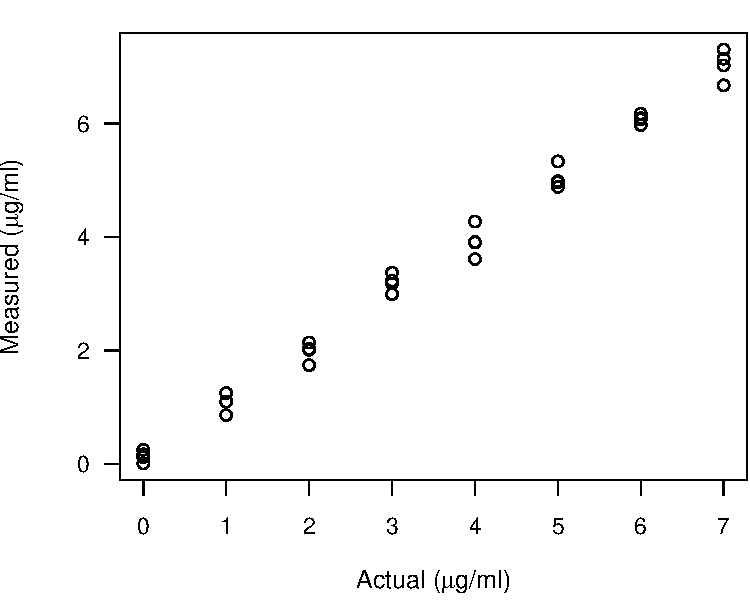
\includegraphics[width=\maxwidth]{figure/arsenic-scatter} \caption[Scatterplot of the arsenic data]{Scatterplot of the arsenic data.\label{fig:arsenic-scatter}}
\end{figure}


\end{knitrout}


% The goal of this work is to extend the methods of calibration to more complicated settings. 
The goal of this work is to extend the methods of calibration to more complicated settings. In Chapter~\ref{chap:nonparametric}, we introduce \textit{semiparametric calibration}. Here we use semiparametric regression methods to estimate the calibration curve and make inference on the unknown $x_0$. The benefit of this approach is that we do not have to specify the exact form of the calibration curve. The downside to this approach is that the estimated calibration curve will be biased, hence, our inference about the unknown $x_0$ will also be biased. We correct for this bias by taking the mixed model approach to smoothing described in, for example, \citet{ruppert_semiparametric_2003}. A small Monte Carlo study shows that this correction is necessary to obtain calibration intervals with coverage probability near the nominal $1-\alpha$ level. We also extend the method of Bayesian linear calibration put forth by \citet{hoadley_bayesian_1970} by allowing for the calibration curve to be estimated semiparametrically as in \citet{crainiceanu_bayesian_2005}. In Chapter~\ref{chp:cal-dependent}, we extend the classical methods of calibration to work with linear mixed-effects models. We also propose a new parametric bootstrap algorithm that can be used to obtain an estimate of the entire sampling distribution of the estimate of $x_0$. We further show how this algorithm can also be used to improve upon the classical methods by removing normality assumptions that may not be satisfied in practice. We use several real datasets to demonstrate and compare our methods.

%This is similar (in spirit) to the parametric bootstrap adjustment proposed by \citet{oman_calibration_1998}, however, Oman's approach is only approximate and does not seem to account for the added variability from the observed response corresponding to the unknown $x_0$.


%% Background ------------------------------------------------------------------

% !Rnw root = Master.Rnw

\chapter{Statistical Background}
\label{chp:background}
This chapter provides an overview of some of the statistical concepts related to inverse estimation. In Section~\ref{sec:notation}, we discuss the basic notational conventions used throughout this dissertation. Section~\ref{sec:lm} introduces the linear regression model. The extension to nonlinear regression models is given in Section~\ref{sec:nonlinear-models}. Section~\ref{sec:penalized-regression-splines} is devoted to penalized regression splines, a type of semiparametric regression model where only part of the model is specified. Finally, in Section~\ref{sec:lmms}, we introduce the linear mixed-effects models, an extension of the \ac{LM} that allows for some of the regression coefficients to vary randomly. 

\section{Notation}
\label{sec:notation}
For the most part, random variables will be denoted by capital letters in a calligraphic font (e.g., $\mc{Y}$). Vectors will be denoted by bold, lowercase letters and matrices will be denoted by bold, uppercase letters. When convenient, we will use the following notation to denote row, column, and diagonal vectors/matrices:
\begin{align*}
  \Big\lbrace_\text{col } x_i \Big\rbrace_{i = 1}^n &= (x_1, \dotsc, x_n)\trans \\
  \Big\lbrace_\text{row } x_i \Big\rbrace_{i = 1}^n &= (x_1, \dotsc, x_n)  \\
  \Big\lbrace_\text{diag } x_i \Big\rbrace_{i = 1}^n &= \diag\left\{x_1, \dotsc, x_n\right\}.
\end{align*}
If $\mc{X}$ is a random variable, then $\mc{X} \sim (\mu, \sigma^2)$ simply means that $\mc{X}$ has some distribution with mean $\E\left\{\mc{X}\right\} = \mu$ and variance $\var\left\{\mc{X}\right\} = \sigma^2$. Estimators and estimates will typically be denoted by the same Greek letter with a hat symbol. For example, depending on the context, $\wh{\bm{\beta}}$ may represent a vector of estimators or their corresponding estimates.

\section{Linear models}
\label{sec:lm}
The linear regression model has been a mainstay of statistics for many years. It has the simple form
\begin{equation}
\label{eqn:linmod}
  \mc{Y}_i = \X_i\trans\bm{\beta} + \epsilon_i, \quad i = 1, \dotsc, n,
\end{equation}
where $\X_i = (x_{i1}, \dotsc, x_{ip})\trans$ is a $p \times 1$ vector of predictor variables for the $i$-th observation, $\bm{\beta} = (\beta_1, \dotsc, \beta_p)\trans$ is a $p \times 1$ vector of fixed (but unknown) regression coefficients, and $\epsilon_i \stackrel{iid}{\sim} (0, \sigma_\epsilon^2)$. Thus, an alternative formulation is to specify the mean response
\begin{equation*}
  \E\left\{\mc{Y}_i|\X\right\} = \X_i\trans\bm{\beta} = \mu_i.
\end{equation*}
Unless stated otherwise, $x_{i1} \equiv 1$ (i.e., the model contains an intercept). It is often convenient to work with the matrix form of \eqref{eqn:linmod}, which is
\begin{equation}
\label{eqn:linmod-matrixform}
  \bc{Y} = \X\bm{\beta} + \bm{\epsilon}, \quad \bm{\epsilon} \sim (\bm{0}, \sigma_\epsilon^2\bm{I}_n), 
\end{equation}
where $\bc{Y} = (\mc{Y}_1, \dotsc, \mc{Y}_n)\trans$ is an $n \times 1$ vector of response variables, $\X = (\X_1, \dotsc, \X_p)\trans$ is an $n \times p$ matrix of predictor variables called the \textit{design matrix}, and $\bm{\epsilon} = (\epsilon_1, \dotsc, \epsilon_n)\trans$ is an $n \times 1$ vector of random errors. Equation~\eqref{eqn:linmod} is special in that the response $\bc{Y}$ is a linear function of the regression parameters $\bm{\beta}$. 

A special case of \eqref{eqn:linmod} arises when $p = 2$ and the distribution for the errors is normal. That is,
\begin{equation}
\label{eqn:linmod-simple}
  \mc{Y}_i = \beta_0 + \beta_1 x_i + \epsilon_i, \quad i = 1, \dotsc, n,
\end{equation}
where $\beta_0$ and $\beta_1$ are the intercept and slope of the regression line, respectively, and $\epsilon_i \stackrel{iid}{\sim} \mc{N}(0, \sigma_\epsilon^2)$. This is called the simple linear regression model and is often used for analyzing calibration data.

Another special case of the linear model \eqref{eqn:linmod} is when $x_{ij} = g_j(x_i)$, $j = 1, \dotsc, p$, where each $g_j(\cdot)$ is a continuous function such as $\sqrt{\cdot}$ or $\log(\cdot)$. For example, a polynomial model of degree $p$ has the form
\begin{equation*}
  \mc{Y}_i = \beta_0 + \beta_1 x_i + \beta_2 x_i^2 + \dotsc + \beta_p x_i^p + \epsilon_i, \quad i = 1, \dotsc, n.
\end{equation*}
Notice that a polynomial model is linear in the parameters even though it is nonlinear in the predictor variable; hence, it is a linear model.

\subsection{Estimating the model parameters}
Estimation of $\bm{\beta}$ in the linear model \eqref{eqn:linmod} can be carried out via \ac{LS}. The ordinary \ac{LS} estimator of $\bm{\beta}$ minimizes the residual sum of squares, 
\begin{equation}
\label{eqn:beta-ols}
  \wh{\bm{\beta}} = \argmin{\bm{\beta}} \norm{\bc{Y} - \X\bm{\beta}}^2 = \left(\X\trans\X\right)^{-1}\X\trans\bc{Y}.
\end{equation}
If we make the additional assumption that the errors are normally distributed, then estimation can also be carried out by the method of \ac{ML}. This has the benefit of simultaneously providing an estimator for both $\bm{\beta}$ and $\sigma_\epsilon^2$. To proceed, we need to maximize the likelihood
\begin{equation*}
  \mc{L}\left(\bm{\beta}, \sigma_\epsilon^2 | \bc{Y}\right) = \left(2\pi\sigma_\epsilon^2\right)^{-n/2}\exp\left\{ -\frac{1}{2\sigma_\epsilon^2}\norm{\bc{Y} - \X\bm{\beta}}^2 \right\},
\end{equation*}
or equivalently, maximize the log-likelihood
\begin{equation*}
  \loglik\left(\bm{\beta}, \sigma_\epsilon^2 | \bc{Y}\right) = -\frac{n}{2}\log\left(2\pi\right) - \frac{n}{2}\log\left(\sigma_\epsilon^2\right) - \frac{1}{2\sigma_\epsilon^2}\norm{\bc{Y} - \X\bm{\beta}}^2.
\end{equation*}
The derivatives of $\loglik(\bm{\beta}, \sigma_\epsilon^2 | \bc{Y})$ with respect to the parameters $\left(\bm{\beta}, \sigma_\epsilon^2\right)$ are
\begin{align*}
  \frac{\partial\loglik}{\partial\bm{\beta}} &= \frac{\X\trans(\bc{Y} - \X\bm{\beta})}{\sigma_\epsilon^2}\\
  \frac{\partial\loglik}{\partial\sigma_\epsilon^2} &= \frac{\norm{\bc{Y} - \X\bm{\beta}}^2}{2\sigma_\epsilon^2} - \frac{N}{2\sigma_\epsilon^2},
\end{align*}
which, upon setting equal to zero and solving yields the \ac{ML} estimators
\begin{align*}
  \wh{\bm{\beta}} &= (\X\trans\X)^{-1}\X\trans\bc{Y} \\
  \wh{\sigma}_\epsilon^2 &= \norm{\bc{Y} - \X\wh{\bm{\beta}}}^2/n
\end{align*}
Fortunately, for the linear model \eqref{eqn:linmod} with normal errors, the \ac{ML} estimator of $\bm{\beta}$ is the same as the \ac{LS} estimator. It is customary to adjust the \ac{ML} estimator of $\sigma_\epsilon^2$ for bias by replacing it with $\wh{\sigma}_\epsilon^2 = \norm{\bc{Y} - \X\wh{\bm{\beta}}}^2/(n-p-1)$.

\subsection{Predictions}
A common use of the fitted regression equation is to make predictions. There are two types of predictions we distinguish:
\begin{enumerate}[(1)]
  \item estimate the mean response when $\X = \X_0$;
  \item predict a future observation corresponding to $\X_0$.
\end{enumerate}
Let $\mu_0$ and $\mc{Y}_0$ be the mean response and future observation of interest, respectively. We will see that the point estimators of $\mu_0$ and $\mc{Y}_0$ are the same, namely the fitted value $\wh{\mu}(x)$. Intuitively, the former should have a smaller standard error since there is less variability in estimating a fixed population parameter than in predicting a future value of a random variable. Consequently, a $100(1 - \alpha)\%$ confidence interval for $\mu_0$ at $\X_0$ will always be smaller than a $100(1 - \alpha)\%$ prediction interval for $\mc{Y}_0$ corresponding to $\X_0$.

Let $\X_0$ be an arbitrary value of $\X$. Suppose we are interested in estimating the mean of $\mc{Y}$ given $\X_0$, $\E\left\{\mc{Y} | \X_0\right\} = \mu_0$. For the linear model \eqref{eqn:linmod}, the \ac{BLUE} of $\mu_0$ is the fitted value $\wh{\mu}_0 = \X_0\trans\wh{\bm{\beta}}$. Furthermore, it is easy to show that
\begin{equation*}
  \E\left\{\wh{\mu}_0\right\} = \X_0\trans\bm{\beta} = \mu_0
\end{equation*}
and
\begin{equation*}
  \var\left\{\wh{\mu}_0\right\} = \sigma_\epsilon^2\left[\X_0\trans\left(\X\trans\X \right)^{-1}\X_0\right] = S^2.
\end{equation*}
Assuming normal errors, it follows that
\begin{equation*}
  \frac{\wh{\mu}_0 - \mu_0}{\wh{\sigma}_\epsilon\sqrt{\left[ \X_0\trans \left( \X\trans\X \right)^{-1} \X_0 \right]}} \sim \mathcal{T}\left(n-p\right).
\end{equation*}
Hence, a $100(1 - \alpha)\%$ confidence interval for the mean response $\mu_0$ is given by
\begin{equation}
\label{eqn:ci-response}
  \X_0\trans\wh{\bm{\beta}} \pm \tquant{1-\alpha/2}{n-p}  \cdot  \widehat{S}.
\end{equation}

Let $\mc{Y}_0$ denote an individual or future observation at the given point $\X_0$. We assume that $\mc{Y}_0 = \X_0\trans\bm{\beta} + \epsilon_0$, where $\epsilon_0 \sim \mc{N}(0, \sigma_\epsilon^2)$ and is independent of $\bm{\epsilon}$. The best predictor of $\mc{Y}_0$ is $\widehat{y}_0 = \X_0\trans\wh{\bm{\beta}}$, the same as $\wh{\mu}_0$, however, the variance of $\widehat{\mc{Y}}_0$ is wider: $\var\left\{\widehat{\mc{Y}}_0\right\} = \sigma_\epsilon^2 + \var\left\{\wh{\mu}_0\right\}$. This is intuitive since there is greater uncertainty in predicting the outcome of a continuous random variable than in estimating a fixed (population) parameter, such as its mean. Under the assumption of normal errors, we have that
\begin{equation*}
  \frac{\widehat{y}_0 - \mc{Y}_0}{\wh{\sigma}_\epsilon\sqrt{\left[1 + \X_0\trans \left( \X\trans\X \right)^{-1} \X_0 \right]}} \sim \mathcal{T}\left(n-p\right),
\end{equation*}
therefore, a $100(1 - \alpha)\%$ prediction interval for $\mc{Y}_0$ is simply
\begin{equation}
\label{eqn:pi-response}
  \X_0\trans\wh{\bm{\beta}} \pm \tquant{1-\alpha/2}{n-p} \sqrt{\wh{\sigma}_\epsilon^2 + \widehat{S}^2}.
\end{equation}
We call \eqref{eqn:pi-response} a prediction interval, as opposed to a confidence interval, since $\widehat{y}_0$ is a prediction for the outcome of the random variable $\mc{Y}_0$.

\section{Nonlinear models}
\label{sec:nonlinear-models}
Often in practice there is an underlying theoretical model relating the response to the predictors, and this model may be nonlinear in the parameters, $\bm{\beta}$. Such nonlinear relationships lead us to the nonlinear regression model. For a single predictor variable, this model is
\begin{equation}
\label{eqn:nonlinemod}
  \mc{Y}_i = \mu(x_i; \bm{\beta}) + \epsilon_i,
\end{equation}
where $\mu(\cdot)$ is a known expectation function that is nonlinear in at least one of the parameters in $\bm{\beta}$, and $\epsilon_i \stackrel{iid}{\sim} \mc{N}(0, \sigma_\epsilon^2)$.

\subsection{Estimating the model parameters}
Borrowing from the notation in \citet{seber_nonlinear_2003}, let $\mu_i(\bm{\beta}) = \mu(x_i; \bm{\beta})$,
\begin{equation*}
  \bm{\mu}(\bm{\beta}) = \left( \mu_1(\bm{\beta}), \dotsc, \mu_N(\bm{\beta}) \right)\trans,
\end{equation*}
and
\begin{equation*}
  \bm{D}(\bm{\beta}) = \frac{\partial\bm{\mu}(\bm{\beta})}{\partial\bm{\beta}\trans} = \Bigg\lbrace_\text{row } \bigg\lbrace_\text{col } \frac{\partial \mu_i(\bm{\beta})}{\partial\beta_j} \bigg\rbrace_{i = 1}^n \Bigg\rbrace_{j = 1}^p.
\end{equation*}
For convenience, let $\widehat{\bm{D}} = \bm{D}(\wh{\bm{\beta}})$.

The approach to estimating $\bm{\beta}$ in the nonlinear model \eqref{eqn:nonlinemod} is similar to the approach in the linear model \eqref{eqn:linmod}. That is, we choose the value of $\bm{\beta}$ that minimizes the residual sum of squares, $\RSS(\bm{\beta})$, defined by
\begin{equation}
\label{eqn:ss-nonlinear}
  \RSS(\bm{\beta}) = \norm{\bc{Y} - \bm{\mu}(\bm{\beta})}^2.
\end{equation}
However, since $\mu(\cdot)$ is nonlinear in the parameters $\bm{\beta}$, minimizing Equation~\eqref{eqn:ss-nonlinear} requires iterative techniques such as methods of \textit{steepest descent} or the \textit{Gauss-Newton} algorithm, which we describe below. 

Given a starting value or current guess $\bm{\beta}^{(0)}$ of the value of $\bm{\beta}$ that minimizes \eqref{eqn:ss-nonlinear}, we can approximate $\mu(x_i; \bm{\beta})$ with a Taylor-series approximation around $\bm{\beta}^{(0)}$. From a first-order Taylor series expansion, we get
\begin{equation}
\label{eqn:taylor-nonlinear}
  \bm{\mu}(\bm{\beta}) \approx \bm{\mu}(\bm{\beta}^{(0)}) + \bm{D}(\bm{\beta}^{(0)})\trans(\bm{\beta} -\bm{\beta}^{(0)}),
\end{equation}
The derivative matrix $\bm{D}(\bm{\beta})$ plays the same role as the design matrix $\X$ in the linear model \eqref{eqn:linmod}, except that $\bm{D}(\bm{\beta})$ may depend on the unknown regression parameters $\bm{\beta}$. Substituting \eqref{eqn:taylor-nonlinear} into Equation~\eqref{eqn:ss-nonlinear}, we get 
\begin{align}
  \RSS(\bm{\beta}) &\approx \norm{\bc{Y} - \bm{\mu}(\bm{\beta}^{(0)}) - \bm{D}(\bm{\beta}^{(0)})(\bm{\beta} - \bm{\beta}^{(0)})}^2 \label{eqn:ss-approximate} \\
  &= \norm{\bc{Y}^{(0)} - \X^{(0)}(\bm{\beta} - \bm{\beta}^{(0)})}^2,
\end{align}
where $\bc{Y}^{(0)} = \bc{Y} - \bm{\mu}(\bm{\beta}^{(0)})$, and $\X^{(0)} = \bm{D}(\bm{\beta}^{(0)})$. Equation~\eqref{eqn:ss-approximate} is of the same form as the sum of squares for the linear model. Based on this approximation, the \ac{LS} estimate of $\bm{\beta}$ is then
\begin{equation*}
  \wh{\bm{\beta}} = \bm{\beta}^{(0)} + \left[ \X^{(0)\trans}\X^{(0)} \right]^{-1}\X^{(0)\trans}\bc{Y}^{(0)}.
\end{equation*}
Hence, given a current approximation $\bm{\beta}^{(k)}$ of $\bm{\beta}$, the updated approximation is 
\begin{equation*}
  \bm{\beta}^{(k + 1)} = \bm{\beta}^{(k)} + \left[ \X^{(k)\trans}\X^{(k)} \right]^{-1}\X^{(k)\trans}\bc{Y}^{(k)}.
\end{equation*}
This process is iterated until a suitable convergence criterion is met. Just as for the linear model, if we assume the errors are normally distributed, then the \ac{ML} estimate of  $\bm{\beta}$ is the same as the \ac{LS} solution.

\subsection{Predictions}
Let $x_0$ be a known value of the predictor $x_0$. The estimate of the mean response $\left\{\mc{Y} | x_0\right\} = \mu(x_0; \bm{\beta})$ is $\wh{\mu}_0 = \mu(x_0; \wh{\bm{\beta}})$. Furthermore, assuming normal errors, an approximate $100(1 - \alpha)\%$ confidence interval for the mean response $\mu_0$ can be obtained as in Equation~\eqref{eqn:ci-response} but with $\widehat{S}^2$ computed as 
\begin{equation*}
  \widehat{S}^2 = \wh{\sigma}_\epsilon^2 \bm{d}_0\trans\left(\widehat{\bm{D}}\trans\widehat{\bm{D}}\right)^{-1}\bm{d}_0,
\end{equation*}
where
\begin{equation*}
  \bm{d}_0 = \left. \bigg\lbrace_\text{row } \frac{\partial \mu\left(x_0; \bm{\beta}\right)}{\partial\beta_i} \bigg\rbrace_{i = 1}^p \right|_{\bm{\beta} = \wh{\bm{\beta}}}.
\end{equation*}

An approximate $100(1 - \alpha)\%$ prediction interval for a future observation is similarly obtained. These intervals, however, rely on the same linear approximation used to compute $\wh{\bm{\beta}}$. For large samples, these intervals are often reliable. When the sample size is small or there is a lot of curvature, these intervals can be highly inaccurate. The \textit{bootstrap} \citep{efron_bootstrap_1979} provides an alternative method of inference under these circumstances.

\section{Smoothing}
\label{sec:penalized-regression-splines}
Let $\bm{x} = \left(x_1, \dotsc, x_n \right)\trans$ be a vector of predictor values and $\bc{Y} = \left( \mc{Y}_1, \dotsc, \mc{Y}_n \right)\trans$ be a vector of response variables. We assume that $\X$ and $\bc{Y}$ are related by the regression model
\begin{equation*}
  \bc{Y} = \mu(\bm{x}) + \bm{\epsilon}, \quad \bm{\epsilon} \sim \mc{N}(\bm{0}, \sigma_\epsilon^2\bm{I}),
\end{equation*}
where $\mu(\cdot)$ is an unknown smooth function. In this section, we discuss a technique for estimating $\mu(\cdot)$ nonparametrically, often referred to as \textit{scatterplot smoothing}, or just \textit{smoothing}. In particular, we will focus on an important class of smoothers called \textit{linear smoothers}. For linear smoothers, the prediction at any point $x$, is a linear combination of the response values: $\wh{\mu}(x) = \bm{\omega}\trans\bc{Y}$, where $\bm{\omega}$ is a constant that does not depend on the response vector $\bc{Y}$. The vector of fitted values $\wh{\bm{\mu}} = \left( \mu(x_1), \dotsc, \mu(x_n) \right)\trans$ can be written in matrix form as $\bm{S}\bc{Y}$, where $\bm{S}$ is an $n \times n$ \textit{smoother matrix}. Examples of linear smoothers include:
\begin{itemize}
  \item running-mean, running-line, and running-polynomial smoothers;
  \item locally-weighted polynomial smoothers (i.e., LOESS);
  \item spline-based smoothers;
  \item kernel smoothers.
\end{itemize}
The remainder of this section discusses spline smoothing, specifically, the \ac{P-spline}.  

Regression splines represent the mean response $\mu(x)$ as a piecewise polynomial of degree $p$. The regions that define each piece are separated by special breakpoints  $\xi_1 < \dotsc < \xi_K$ called \textit{knots}. By increasing $p$ or the number of knots, the family of curves becomes more flexible; thus, as shown in Figure~\ref{fig:sinc-example}, we can easily handle any level of complexity. 

\begin{knitrout}
\definecolor{shadecolor}{rgb}{0.969, 0.969, 0.969}\color{fgcolor}\begin{figure}[!htb]

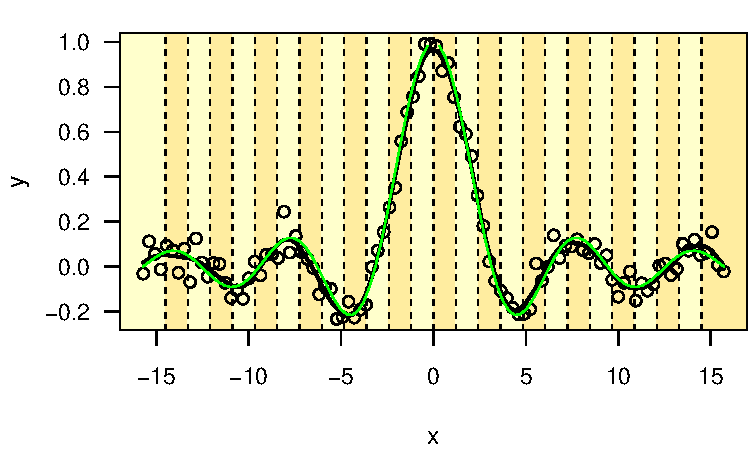
\includegraphics[width=\maxwidth]{figure/sinc-example} \caption[Unnormalized sinc function example]{Unnormalized sinc function example. Scatterplot of 100 observations generated from a regression model with mean response $\mu(x) = \sin(x)/x$ (green line) and i.i.d. $\mc{N}(0, 0.05^2)$ errors. The solid line shows a quadratic \ac{P-spline} fit with smoothing parameter $\lambda = 0.9986$. The dotted lines indicate the position of the knots $\xi_k$.\label{fig:sinc-example}}
\end{figure}


\end{knitrout}


A $p$-th degree spline function has the form
\begin{equation}
\label{eqn:spline-model}
  \mu(x) = \beta_0 + \beta_1x + \dotsc + \beta_px^p + \sum_{k = 1}^K \alpha_k(x - \xi_k)_+^p,
\end{equation}
where the notation $a_+$ denotes the positive part of $a$, that is, $a_+ = a \cdot I(a \ge 0)$. Many methods for choosing the number and location of the knots are given in the literature (see, for example, \citet{ruppert_selecting_2002} and the references therein). Let $n_x$ be the number of unique $x_i$. A reasonable choice for the number of knots \citep[pg. 126]{ruppert_semiparametric_2003} is $K = \min(n_x/4, 35)$ with knot locations
\begin{equation*}
  \xi_k = \left(\frac{k+1}{K+2}\right)\text{-th sample quantile of the unique } x_i, \quad k = 1, \dotsc, K.
\end{equation*}
The idea is to choose enough knots to capture the structure of $\mu(x)$. If both $p$ and $K$ are too large, we run the risk of overfitting (i.e., low bias and high variance). If $K$ is too small then the resulting fit may be too restrictive (i.e., low variance but high bias). There is rarely the need to go beyond a cubic polynomial model and so typical choices for $p$ are 1, 2, or 3.

In matrix form, the polynomial spline model is
\begin{equation}
\label{eqn:spline-model-matrix}
  \bc{Y} = \X\bm{\beta} + \bm{\epsilon}, \quad \bm{\epsilon} \sim (\bm{0}, \sigma_\epsilon^2\bm{I}),
\end{equation}
where 
\begin{equation*}
  \X = 
    \begin{bmatrix}
      1 & x_1 & \cdots & x_1^p & (x_1-\xi_1)_+^p & \dotsc & (x_1-\xi_K)_+^p \\  
      \vdots & \vdots & \ddots & \vdots & \vdots & \ddots & \vdots \\
      1 & x_n & \cdots & x_n^p & (x_n-\xi_1)_+^p & \dotsc & (x_n-\xi_K)_+^p
    \end{bmatrix}.              
\end{equation*}
Equation~\eqref{eqn:spline-model-matrix} has the same form as the linear model \eqref{eqn:linmod-matrixform}. The ordinary least squares fit, however, will be too ``wiggly.'' The idea behind penalized spline regression is to shrink the coefficients $\alpha_k$ by imposing a penalty on their size, thereby limiting their impact on the estimated response curve. The estimated coefficients minimize the penalized residual sum of squares
\begin{equation}
\label{eqn:pss}
  \PSS = \norm{\bc{Y} - \X\bm{\beta}}^2 + \lambda^{2p}\bm{\beta}\trans\bm{D}\bm{\beta},
\end{equation}
where $\bm{D} = \diag\left\{\bm{0}_{(p+1) \times (p+1)}, \bm{I}_{K \times K}\right\}$. The penalized least squares solution is then
\begin{equation}
\label{eqn:pss-solution}
  \wh{\bm{\beta}}_\lambda = \argmin{\bm{\beta}} \norm{\bc{Y} - \X\bm{\beta}}^2 + \lambda^{2p}\bm{\beta}\trans\bm{D}\bm{\beta} = \left( \X\trans\X + \lambda^{2p}\bm{D} \right)^{-1}\X\trans\bc{Y}.
\end{equation}
Here $\lambda \ge 0$ is a \textit{smoothing parameter} that controls the wiggliness of the fit. Small values of $\lambda$ produce wiggly curves while larger values  produce smoother curves. The term $\lambda^{2p}\bm{\beta}\trans\bm{D}\bm{\beta}$ is called the \textit{roughness penalty}. If $\bm{D} = \bm{I}$, then the penalized least squares solution \eqref{eqn:pss-solution} is equivalent to the ridge regression estimate of $\bm{\beta}$. The roughness penalty can also be written as $\lambda^{2p}\norm{\bm{\alpha}}^2$, where $\bm{\alpha} = (\alpha_1, \dotsc, \alpha_K)\trans$ is the vector of coefficients for the spline basis functions. Hence, \acp{P-spline} enforce a penalty on the $\ell^2$-norm of $\bm{\alpha}$, so none of the polynomial coefficients are penalized (See Figure~\ref{fig:sinc-example-2})! 

\begin{knitrout}
\definecolor{shadecolor}{rgb}{0.969, 0.969, 0.969}\color{fgcolor}\begin{figure}[!htb]

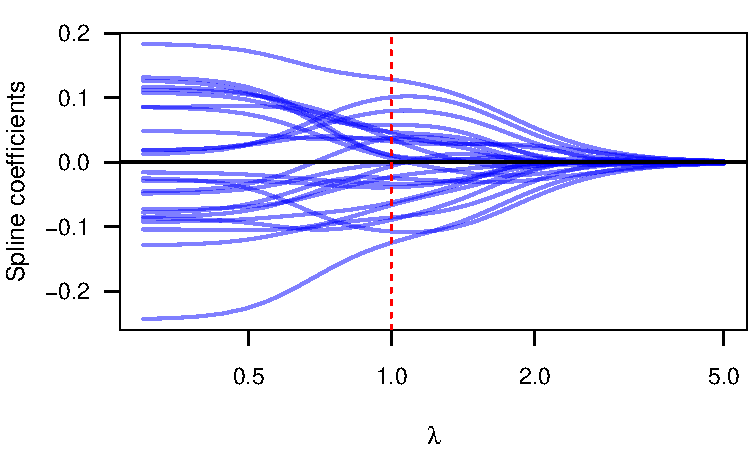
\includegraphics[width=\maxwidth]{figure/sinc-example-2} \caption[Sinc function spline coefficient profiles]{Profiles of spline coefficients as the smoothing parameter $\lambda$ is varied. Coefficients are plotted versus $\lambda$. A vertical line is drawn at $\lambda = 0.9986$.\label{fig:sinc-example-2}}
\end{figure}


\end{knitrout}


The fitted values are given by $\wh{\bm{\mu}} = \bm{S}_\lambda \bc{Y}$, where $\bm{S}_\lambda = \X\left( \X\trans\X + \lambda^{2p}\bm{D} \right)^{-1}\X\trans$. From this point forward, we will drop the subscript $\lambda$ on the smoother matrix and just write $\bm{S}$. The smoothing parameter $\lambda$ is unknown but can be specified a priori. However, it is often beneficial to let the data determine the appropriate amount of smoothness. To this end, cross-validation techniques are often used to estimate $\lambda$ from the given data. In Chapter~\ref{chp:cal-dependent}, we discuss an alternative approach to \acp{P-spline} that automatically selects an appropriate amount of smoothness.

\subsection{Inference for linear smoothers}
\label{sec:pspline-inference}
Consider the general heteroscedastic error model
\begin{equation*}
  \mc{Y}_i = \mu(x_i) + \epsilon_i, \quad \epsilon_i \stackrel{iid}{\sim} (0, \sigma_\epsilon^2), \quad i = 1, \dotsc n,
\end{equation*}
where $\mu(\cdot)$ is an unknown smooth function. Let $\wh{\mu}(x)$ be an estimate of $\mu(\cdot)$ based on a linear smoother. The covariance matrix of the vector of fitted values $\wh{\bm{\mu}} = \bm{S}\bc{Y}$ is 
\begin{equation}
\label{eqn:cov}
  \var\left\{\wh{\bm{\mu}}\right\} = \bm{S}\left( \sigma_\epsilon^2\bm{I} \right) \bm{S}\trans = \sigma_\epsilon^2   \bm{S}\bm{S}\trans.
\end{equation}
For a single point, the quantity $Q = \left[ \wh{\mu}(x) - \mu(x) \right]/\se\left\{ \wh{\mu}(x) \right\}$ is approximately pivotal---the distribution is free of unknown parameters, at least for sufficiently large sample size $n$. Therefore, assuming $\bm{\epsilon} \sim \mc{N}(\bm{0}, \sigma_\epsilon^2\bm{I})$, Equation~\eqref{eqn:cov} can be used to form confidence intervals and prediction intervals. Note, however, that $\E\left\{\wh{\bm{\mu}}\right\} = \X\left( \X\trans\X + \lambda^{2p}\bm{D} \right)^{-1}\X\trans\X\bc{Y}$; hence, $\wh{\mu}(x)$ is a biased estimator of $\mu(x)$. Unless the bias is negligible, the confidence intervals discussed here only cover $\E\left\{\wh{\mu}(x)\right\}$ with $100(1 - \alpha)\%$ confidence. This problem is remedied for \acp{P-spline} in Chapter~\ref{chap:nonparametric} where we discuss an alternative approach using mixed model methodology.  

Let $x$ be an arbitrary value of the explanatory variable. Recall that, for linear smoothers, the fitted value $\wh{\mu}(x)$ can be written as $\bm{\omega}\trans\bc{Y}$, a linear combination of the response variables. The variance of $\wh{\mu}(x)$ is just $\var\left\{\bm{\omega}\trans\bc{Y}\right\} = \sigma_\epsilon^2\bm{\omega}\trans\bm{\omega}$. Given an estimate $\wh{\sigma}_\epsilon^2$ of $\sigma_\epsilon^2$, an approximate $100(1 - \alpha)\%$ confidence interval for $\mu(x)$ is given by 
\begin{equation*}
  \wh{\mu}(x) \pm \tquant{1-\alpha/2}{df} \wh{\sigma}_\epsilon \sqrt{\bm{\omega}\trans\bm{\omega}},
\end{equation*}
where $df = n - 2\tr\left( \bm{S} \right) + \tr\left( \bm{S}\bm{S}\trans \right)$. For sufficiently large sample size $n$, the quantity $\tquant{1-\alpha/2}{df}$ can be replaced with $z_{1-\alpha/2}$, the $1-\alpha/2$ quantile of a standard normal distribution. Similarly, A $100(1-\alpha)\%$ prediction interval for a new observation is 
\begin{equation*}
  \wh{\mu}(x) \pm \tquant{1-\alpha/2}{df} \wh{\sigma}_\epsilon \sqrt{1 + \bm{\omega}\trans\bm{\omega}}.
\end{equation*}

\section{Linear mixed effects models}
\label{sec:lmms}
Mixed effects models (henceforth referred to as just mixed models) represent a large and growing area of statistics. In this section, we only summarize the key aspects of a special kind of mixed model called the \ac{LMM}. The extension to nonlinear mixed effects models and generalized linear mixed effects models is discussed in  \citet{pinheiro_mixed_2009} and \citet{mcculloch_generalized_2008}, respectively. Mixed models are useful for describing \textit{grouped data} where observations belonging to the same group are correlated. One way of accounting for such correlation is by introducing random effects into the model which induces a particular correlation structure on the response vector. Different random effects structures induce different correlation structures on the response. 

The \ac{LMM} extends the basic \ac{LM} (Equation~\eqref{eqn:linmod-matrixform}) to
\begin{equation}
\label{eqn:linmod-mixed}
  \bc{Y} = \X\bm{\beta} + \Z\bm{\alpha} + \bm{\epsilon},
\end{equation}
where $\X$ and $\Z$ are known design matrices, $\bm{\beta}$ is a vector of fixed effects, $\bm{\alpha}$ is a vector of random effects distributed as $\bm{\alpha} \sim \mc{N}(0, \bm{G})$, and $\bm{\epsilon}$ is a vector of random errors distributed as $\bm{\epsilon} \sim \mc{N}(\bm{0}, \bm{R})$. Further, it is assumed that the random effects and errors are mutually independent, that is, $\bm{\alpha} \indep \bm{\epsilon}$.

Estimating the fixed effects $\bm{\beta}$ is rather straightforward and does not require normality. Note that $\bc{Y} = \X\bm{\beta} + \bm{\mc{E}}$, where $\E\left\{\bm{\mc{E}}\right\} = \bm{0}$ and $\var\left\{\bm{\mc{E}}\right\} = \Z\bm{G}\Z\trans + R = \bm{V}$. Assuming normality, the log-likelihood (ignoring constants) is given by
\begin{equation}
\label{eqn:lmm-loglik-long}
  \loglik\left(\bm{\beta}, \bm{\theta}\right) = -\frac{1}{2}\log\left|\bm{V}\right| - \frac{1}{2}\left(\bc{Y} - \X\bm{\beta}\right)\trans\bm{V}^{-1}\left(\bc{Y} - \X\bm{\beta}\right),
\end{equation}
where $\bm{\theta}$ is a vector containing the unique elements of $\bm{V}$. Equating the partial derivative of $\loglik\left(\bm{\beta}, \bm{\theta}\right)$, with respect to the parameter $\bm{\beta}$, yields the so-called \ac{GLS} estimator
\begin{equation}
\label{eqn:beta-gls}
  \wt{\bm{\beta}} = \left(\X\trans\bm{V}^{-1}\X\right)^{-1}\X\trans\bm{V}^{-1}\bc{Y}.
\end{equation}
Notice, however, that the \ac{GLS} estimator---which happens to be the \ac{BLUE} of $\bm{\beta}$---depends on the variance-covariance matrix $\bm{V}$. Since this is rarely available in practice, the usual procedure is to estimate $\bm{V}$ and then plug this into Equation~\eqref{eqn:beta-gls}. In other words, if $\widehat{\bm{V}}$ is an estimate of $\bm{V}$, then the \ac{EBLUE} of $\bm{\beta}$ is 
\begin{equation}
\label{eqn:beta-egls}
  \wh{\bm{\beta}} = \left(\X\trans\widehat{\bm{V}}^{-1}\X\right)^{-1}\X\trans\widehat{\bm{V}}^{-1}\bc{Y}.
\end{equation}
This causes some difficulties, mostly in terms of finite-sample inference, since there is no simple way to account for the variability of $\widehat{\bm{V}}$ when calculating $\var\left\{\wh{\bm{\beta}}\right\}$. See, for example, \citet[pp. 165-167]{mcculloch_generalized_2008}.

A technique known as \textit{best linear unbiased prediction} is commonly used to estimate the random effects $\bm{\alpha}$. It can be shown \citep{henderson_sire_1973} that the \ac{BLUE} of $\bm{\beta}$ and the \ac{BLUP} of $\bm{\alpha}$, denoted $\wt{\bm{\alpha}}$, can be determined simultaneously as the solutions to a penalized least squares problem,
% \begin{equation}
% \label{eqn:henderson's-justification}
%   (\bc{Y} - \X\bm{\beta} - \Z\bm{\alpha})\trans\bm{R}^{-1}(\bc{Y} - \X\bm{\beta} - \Z\bm{\alpha}) + \bm{\alpha}\trans\bm{G}^{-1}\bm{\alpha}.
% \end{equation} 
% Henderson showed that the minimum of \eqref{eqn:henderson's-justification} occurs at
\begin{align}
  \begin{bmatrix} 
    \wt{\bm{\beta}} \\ \wt{\bm{\alpha}} 
  \end{bmatrix} &= \argmin{\bm{\beta}, \bm{\alpha}} (\bc{Y} - \X\bm{\beta} - \Z\bm{\alpha})\trans\bm{R}^{-1}(\bc{Y} - \X\bm{\beta} - \Z\bm{\alpha}) + \bm{\alpha}\trans\bm{G}^{-1}\bm{\alpha} \label{eqn:henderson} \\
  &= \bm{\Omega}(\bm{\Omega}\trans\bm{R}^{-1}\bm{\Omega} + \bm{D})\bm{\Omega}\trans\bm{R}^{-1}\bc{Y} \nonumber,
\end{align}
where $\wt{\bm{\beta}}$ is as in \eqref{eqn:beta-gls}, $\wt{\bm{\alpha}} = \bm{G}\Z\trans\bm{V}^{-1}\left(\bc{Y} - \X\wt{\bm{\beta}}\right)$, $\bm{\Omega} = \left(\X; \Z\right)$, and $\bm{D} = \diag\left\{\bm{0}_{p \times p}, \bm{G}^{-1}\right\}$.
For the special case $\bm{R} = \sigma_\epsilon^2\bm{I}$ and $\bm{G} = \sigma_\alpha^2\bm{I}$, the \ac{PSS}---the minimand in Equation~\eqref{eqn:henderson}--- reduces to
\begin{equation}
\label{eqn:lmm-pss}
  \frac{1}{\sigma_\epsilon^2}\norm{\bc{Y} - \X\bm{\beta} - \Z\bm{\alpha}}^2 +\frac{1}{\sigma_\alpha^2}\norm{\bm{\alpha}}^2.
\end{equation}
Similar to the \ac{EBLUE} of $\bm{\beta}$, the \ac{EBLUP} of $\bm{\alpha}$ is just the \ac{BLUP} $\wt{\bm{\alpha}}$ with $\bm{G}$ and $\bm{V}$ replaced with their respective estimates, $\widehat{\bm{G}}$ and $\widehat{\bm{V}}$:
\begin{equation}
\label{eqn:alpha-eblup}
  \wh{\bm{\alpha}} = \widehat{\bm{G}}\Z\trans\widehat{\bm{V}}^{-1}\left(\bc{Y} - \X\wh{\bm{\beta}}\right).
\end{equation} 
In a similar fashion, the \ac{BLUP} and \ac{EBLUP} of the mean response are given, respectively, by the equations
\begin{align}
  \widetilde{\bm{\mu}} &= \X\wt{\bm{\beta}} + \Z\wt{\bm{\alpha}}, \label{eqn:mu-blup} \\
  \wh{\bm{\mu}} &= \X\wh{\bm{\beta}} + \Z\wh{\bm{\alpha}}. \label{eqn:mu-eblup}
\end{align}
Note that the \ac{EBLUP} $\wh{\bm{\mu}}$ is just the fitted values.

Obviously, estimating $\wt{\bm{\beta}}$ and $\wt{\bm{\alpha}}$, requires knowledge of the variance-covariance matrices $\bm{G}$ and $\bm{R}$, which are generally unknown. In practice, we often restrict these matrices to have a simple form, usually involving only a few unknown parameters, earlier denoted by $\bm{\theta}$. These parameters can be estimated via \ac{ML} estimation. \ac{ML} estimators of the variance components $\bm{\theta}$, however, tend to become badly biased as the number of fixed effects in the model increases. A more effective approach, known as \ac{REML} estimation, is often used instead (see, for example, \citet[chap. 6]{mcculloch_generalized_2008}). 


%% Literature review -----------------------------------------------------------

% !Rnw root = Master.Rnw

\chapter{Overview of Statistical Calibration}
\label{chap:lit-review}
In this chapter, we present a thorough overview of calibration as it pertains to our goals for this dissertation. Although we cannot cover every aspect of calibration in this chapter, we have attempted to provide an extensive bibliography for the interested reader. The main themes of this chapter are going to be point estimation and interval estimation.

\section{Controlled Calibration vs. Natural Calibration}
\label{sec:controlled-vs-natural}
Calibration experiments can be classified as one of two types: \textit{controlled calibration} experiments and \textit{natural calibration} experiments. In controlled calibration, the predictor values are held fixed by the experimenter (i.e., $x$ is not considered a random variable). In this case, the predictor values are chosen to cover the experimental range of interest and the response is often replicated a number of times at each design point (see, for example, the arsenic data plotted in Figure~\ref{fig:arsenic-scatter}). In contrast, the $n$ observations $(x_i, y_i)$ in a natural calibration experiment are considered a random sample from some bivariate distribution: $(\mc{X}, \mc{Y}) \sim g(x, y)$, where $g$ is typically assumed to be a bivariate normal distribution. In summary, the values of the independent variable are either preselected or held fixed in controlled calibration and randomly sampled from a population of values in natural calibration. Distinguishing between these two types of calibration experiments is important, especially from an inferential standpoint, as emphasized in the papers by \citet{brown_multivariate_1982} and \citet{brown_measurement_1993}.

\section{Point estimation}
\label{sec:point-estimation}

Here, we discuss point estimation of $x_0$ for the linear calibration problem, that is, when the calibration curve has the form of the simple linear regression model. The two most popular estimators of $x_0$ are the \textit{classical estimator} and the \textit{inverse estimator}. The classical estimator, which dates back to \citet{eisenhart_interpretation_1939}, is based on inverting the calibration curve at $y_0$ (i.e., solving the fitted regression equation for $x_0$) and is easily extended to polynomial and nonlinear calibration problems. The inverse estimator, as we will see in Section~\ref{sec:bayesian}, is more useful under a specific Bayesian framework.  

\subsection{The classical estimator}
Suppose we have $n$ observations $(x_i, \mc{Y}_i)$. We assume the $x_i$'s were measured without error. (The case where there is error in both variables is discussed in \citet{carroll_effect_1986}.) Generally, the model considered is of the form
\begin{equation}
\label{eqn:nonlinear-model}
  \mc{Y}_i = \mu\left(x_i; \bm{\beta}\right) + \epsilon_i, \quad i = 1, \dotsc, n,
\end{equation}  
where $\mu = \E\left\{\mc{Y} | x\right\}$ is a known expectation function, $\bm{\beta}$ is a vector of $p$ unknown regression parameters, and the errors are independent and identically distributed (i.i.d.) normal random variables: $\epsilon_i \stackrel{iid}{\sim} \mc{N}(0, \sigma_\epsilon^2)$. We consider the linear calibration problem, a special case of Equation~\eqref{eqn:nonlinear-model} with $\E\left\{\mc{Y} | x\right\} = \beta_0 + \beta_1 x$. 

The fitted calibration line is given as
\begin{equation}
\label{eqn:fitted-slr-model}
  \wh{\mu} = \wh{\beta}_0 + \wh{\beta}_1 x,
\end{equation}
where $\wh{\beta}_0$ and $\wh{\beta}_1$ are the \ac{ML} estimates of $\beta_0$ and $\beta_1$, respectively. If we observe $\mc{Y}_0 = y_0$, where $\mc{Y}_0 \sim \mc{N}(\beta_0 + \beta_1 x_0, \sigma_\epsilon^2)$, then the obvious estimate of $x_0$ is obtained by inverting the calibration line:
\begin{equation}
\label{eqn:x0-mle}
  \wh{x}_0 = \mu^{-1}(y_0; \bm{\beta}) = \frac{y_0 - \wh{\beta}_0}{\wh{\beta}_1} = \bar{x} + \frac{S_{xx}}{S_{xy}}(y_0 - \bar{y}),
\end{equation}
where $S_{xy} = \sum(x_i-\bar{x})(y_i-\bar{y})$, and $S_{xx} = \sum(x_i-\bar{x})^2$. Under the assumption of i.i.d. normal errors, Equation~\eqref{eqn:x0-mle} is the \ac{ML} estimate of $x_0$. More generally, suppose in addition to the standards 
\begin{equation*}
  (x_1, \mc{Y}_1), (x_2, \mc{Y}_2), \dotsc, (x_n, \mc{Y}_n),
\end{equation*}
we have $m$ unknowns
\begin{equation*}
  (x_0, \mc{Y}_{n+1}), (x_0, \mc{Y}_{n+2}), \dotsc, (x_0, \mc{Y}_{n+m}).
\end{equation*}
We assume that the $\mc{Y}_i$'s ($i = 1, \dotsc, n$) are independent and distributed according to
\begin{equation*}
  \mc{Y}_i \sim \left\{
  \begin{array}{l l}
    \mc{N}(\beta_0+\beta_1 x_i, \sigma_{\text{I}}^2), & \quad i=1,2,\dotsc,n \smallskip \\
    \mc{N}(\beta_0+\beta_1 x_0, \sigma_{\text{II}}^2), & \quad i=n+1,n+2,\dotsc,n+m
  \end{array} \right..
\end{equation*}
In practice, assuming that $\sigma_{\text{I}}^2 = \sigma_{\text{II}}^2$ is often reasonable; however, some authors (e.g., \citet[p. 659]{berkson_estimation_1969}), have argued otherwise. In controlled calibration, one could argue that the variance in the first stage, $\sigma_{\text{I}}^2$, may be smaller than the variance from the second stage, $\sigma_{\text{II}}^2$, since the standards were likely collected under more highly controlled conditions. For example, the standards in the arsenic data may have been collected in a laboratory under tightly controlled conditions, while the measurement made on the new sample was likely made in the field (e.g., a lake) and therefore susceptible to greater measurement error. 

The log-likelihood for all $n + m$ observations is
\begin{equation*}
\begin{split}
  \loglik\left(\beta_0, \beta_1, \sigma_\epsilon^2, x_0\right) = &-\frac{n+m}{2}\log(2\pi\sigma_\epsilon^2)-\\ &\quad \frac{1}{2\sigma_\epsilon^2}\left[\sum_{i=1}^n(\mc{Y}_i-\beta_0-\beta_1x_i)^2 + \sum_{i=n+1}^{n+m}(\mc{Y}_i-\beta_0-\beta_1x_0)^2\right].
\end{split}
\end{equation*}
Equating the partial derivatives of $\loglik\left(\beta_0, \beta_1, \sigma_\epsilon^2, x_0\right)$ to zero and solving for the parameters produces the usual \ac{ML} estimators of the slope and intercept, but also yields
\begin{align}
  \wh{x}_0 &= \frac{\wb{\mc{Y}}_0-\wh{\beta}_0}{\wh{\beta}_1} \label{eqn:x0-mle2} \\
  \wh{\sigma}_\epsilon^2 &= \frac{1}{n+m-3}\left[\sum_{i=1}^n\left(\mc{Y}_i-\wh{\beta}_0-\wh{\beta}_1 x_i\right)^2 + \sum_{i=n+1}^{n+m}\left(\mc{Y}_i-\wb{\mc{Y}}_0\right)^2\right] \label{eqn:pooledvar},
\end{align}
where $\wb{\mc{Y}}_0 = m^{-1}\sum_{i=n+1}^{n+m}\mc{Y}_i$. Equation~\eqref{eqn:x0-mle2} is known as the classical estimator of $x_0$. The mean of $\wh{x}_0$ does not exist, and it has infinite variance and mean squared error (MSE). This is not too surprising since Equation~\eqref{eqn:x0-mle2} is a ratio of jointly normal random variables (recall that a standard Cauchy distribution, which does not have any finite moments, results from the ratio of standard normal random variables). Also, note that the pooled estimate $\wh{\sigma}_\epsilon^2$, Equation~\eqref{eqn:pooledvar}, is a weighted average of the estimates of $\sigma_\epsilon^2$ from the first and second stages of the calibration experiment. 

The sampling distribution of $\wh{x}_0$ is quite complicated. Fortunately, its derivation is not necessary for setting a $100(1-\alpha)\%$ confidence interval on $x_0$ (see Section~\ref{sec:interval-estimation}). Nonetheless, the resulting distribution has been studied by \citet{fieller_distribution_1932}, \citet{hinkley_ratio_1969}, \citet{buonaccorsi_design_1986}, and \citet{pham-gia_density_2006}, among others. The paper by \citet{pham-gia_density_2006} gives a closed-form expression for the density of the ratio of jointly normal random variables. \citet{buonaccorsi_design_1986} showed that a sufficient condition for unimodality of the sampling distribution of $\wh{x}_0$ is
\begin{equation*}
  (x_0 - \bar{x})^2 < 5.094 \left(\frac{\sigma}{\beta_1}\right)^2 \left( \frac{1}{m} + \frac{1}{n} \right).
\end{equation*}
A similar result also holds for the posterior of $x_0$ in the \citet{hunter_bayesian_1981} approach to Bayesian linear calibration (see Section~\ref{sec:bayesian}). Unimodality here is important since some confidence intervals (e.g. the Wald interval of Section~\ref{sec:wald_int}) are derived under the assumption that the sampling distribution of $\wh{x}_0$ is asymptotically normal. 

\subsection{The inverse estimator}
\label{sec:inverse-estimator}
The classical estimator involves regressing $y$ on $x$ and solving the fitted regression equation for the unknown $x_0$. The inverse estimator, however, uses the regression of $x$ on $y$ to obtain
\begin{equation}
\label{eqn:x0-inverse}
  \wt{x}_0 = \wh{\gamma}_0 + \wh{\gamma}_1 \bar{y}_0 = \bar{x} + \frac{S_{xy}}{S_{yy}}(\bar{y}_0 - \bar{y}),
\end{equation}
where $\wh{\gamma}_0$ and $\wh{\gamma}_1$ are least squares (LS) estimates, and $S_{yy} = \sum(y_i-\bar{y})^2$. After a bit of algebra, Equation~\eqref{eqn:x0-inverse} can be re-written as
\begin{equation}
\label{eqn:x0-inverse2}
  \wt{x}_0 = \left(1-\frac{S_{xy}^2}{S_{xx}S_{yy}}\right)\bar{x} + \frac{S_{xy}^2}{S_{xx}S_{yy}}\wh{x}_0 = \left(1-R^2\right)\bar{x} + R^2\wh{x}_0,
\end{equation}
where $R^2$ is the coefficient of determination computed from \eqref{eqn:fitted-slr-model}. This shows $\wt{x}_0$ as a weighted average of the \ac{ML} estimator $\wh{x}_0$ and $\bar{x}$; hence, the inverse estimator takes into account previous information about $x_0$ (this is relevant to Section~\ref{sec:bayesian} where the inverse estimator is shown to be Bayes with respect to a certain prior on $x_0$). Also, when the error variance is zero, $R^2 = 1$ and $\wt{x}_0 = \wh{x}_0$. 

Inference based on this approach, at least from the frequentist perspective, is justifiable only if the observations $(x_i, y_i)$ are sampled from a bivariate distribution (i.e., a natural calibration experiment). In controlled calibration experiments, $x$ is held fixed and the classical estimator is mostly preferred. Nonetheless, much effort has gone into justifying the use of the inverse estimator in controlled calibration (see, for example, \citet{krutchkoff_classical_1967} and more recently \citet{kannan_comparison_2007}).

\subsection{Criticisms and other estimators}
\label{sec:criticisms}
Using extensive Monte Carlo simulations, \citet{krutchkoff_classical_1967} argued that the inverse estimator \eqref{eqn:x0-inverse} had a uniformly smaller \ac{MSE} than the classical estimator \eqref{eqn:x0-mle}. His experiments considered both normal and non-normal error distributions. This sparked controversy in the statistical community resulting in a renewed interest in the inverse estimator for controlled calibration. In a later paper \citep{krutchkoff_classical_1969}, Krutchkoff concluded that the classical approach is superior for large sample sizes when extrapolating beyond the range of observations. 

When the error distribution is normal and $n \ge 4$, the inverse estimator has finite \ac{MSE} \citep{oman_exact_1985}; whereas the classical estimator has infinite \ac{MSE} for finite $n$ \citep{williams_note_1969}. Furthermore, \citet{williams_note_1969} argued that \ac{MSE} is an inappropriate criterion for comparing the two estimators by establishing that ``...no unbiased estimator [of $x_0$] will have finite variance.'' \citet{halperin_inverse_1970} agreed with Williams and suggested the use of the \textit{Pitman closeness} criterion (\citealt{pitman_closest_1937}; \citealt[pg. 290]{mood_introduction_1974}) instead. For a parameter $\phi$ with parameter space $\Phi$, an estimator $T_1$ is said to be Pitman closer (to $\phi$) than another estimator $T_2$ if for all $\phi \in \Phi$,
\begin{equation}
%\label{eqn:pitman}
  \Prob_\phi\left(|T_1 - \phi| < |T_2 - \phi|\right) > 0.5.
\end{equation}
Unlike the \ac{MSE} criterion, Pitman closeness takes into consideration the correlation between the two estimators being compared (here, they are perfectly correlated). With respect to the Pitman closeness criterion, Halperin claimed that the classical estimator is superior both outside and within the range of predictor values; though, Halperin's conclusions were based on asymptotic approximations. In addition, Halperin also compared the two estimators in terms of consistency and \ac{MSE} of the relevant asymptotic distributions, showing that Krutchkoff's findings were only true for a closed interval around $\bar{x}$. The width of this interval depends on the product of the standardized slope and standard deviation of the predictor values, $\sigma_x$. Halperin also preferred the classical estimator on the basis that it yields an exact $100(1 - \alpha)\%$ confidence region for $x_0$ (see Section~\ref{sec:inversion-interval}). In response, \citet{krutchkoff_calibration_1972} used the Pitman closeness criterion in Monte Carlo simulations and obtained the opposite results; that is, the inverse estimator was overall superior to the classical estimator. The contradiction seems to stem from the range of predictor values considered by both authors.

The classical and inverse estimators cannot be compared through exact moments; however, one can easily examine their asymptotic properties. \citet{berkson_estimation_1969} established that the classical estimator is asymptotically unbiased while the inverse estimator is not. He derives formulas for the asymptotic bias, variance, and \ac{MSE} of both estimators. \citet{shukla_problem_1972} extended these formulas to an accuracy of $O(n^{-1})$:
\begin{align*}
  \bias\left\{\wh{x}_0\right\} &\approx \frac{\sigma_\epsilon^2}{S_{xx}\beta_1^2}(x_0 - \bar{x}) \\
  \var\left\{\wh{x}_0\right\} &\approx \frac{\sigma_\epsilon^2}{\beta_1^2}\left[ \frac{1}{m} + \frac{1}{n} + \frac{(x_0 - \bar{x})^2}{S_{xx}} + \frac{3\sigma_\epsilon^2}{m S_{xx} \beta_1^2} \right] \\
  \MSE\left\{\wh{x}_0\right\} &\approx \frac{\sigma_\epsilon^2}{\beta_1^3}\left[ \frac{1}{m} + \frac{1}{n} + \frac{(x_0 - \bar{x})^2}{S_{xx}} + \frac{3\sigma_\epsilon^2}{m S_{xx} \beta_1^2} \right] \\
  \bias\left\{\wt{x}_0\right\} &\approx \frac{\sigma_\epsilon^2}{\beta_1^2\sigma_x^2\theta}(\bar{x}-x_0) - \frac{2\sigma_\epsilon^2(\bar{x}-x_0)}{n\beta_1^2\sigma_x^2\theta^3} \\
  \var\left\{\wt{x}_0\right\} &\approx \frac{\sigma_\epsilon^2}{\beta_1^2\theta^2}\left[ \frac{1}{m} + \frac{1}{n} + \frac{(x_0 - \bar{x})^2}{S_{xx}} + \frac{\sigma_\epsilon^2(\theta^2-2\theta+6)}{m S_{xx}\beta_1^2\theta^2} \right] \newln - \frac{2\sigma^4(x_0-\bar{x})^2}{n\theta^4\beta_1^4\sigma_x^4} \\
  \MSE\left\{\wt{x}_0\right\} &\approx \frac{\sigma_\epsilon^2}{\beta_1^2\theta^2}\left[ \frac{1}{m} + \frac{1}{n} + \frac{(x_0 - \bar{x})^2}{S_{xx}} + \frac{\sigma_\epsilon^2(\theta^2-2\theta+6)}{m S_{xx}\beta_1^2\theta^2} \right] \newln - \frac{\sigma^4(x_0-\bar{x})^2}{\theta^2\beta_1^4\sigma_x^4}\left(1-\frac{6}{n\theta^2}\right),
\end{align*}
where $\sigma_x^2 = S_{xx}/(n-1)$ and $\theta = 1 + \sigma_\epsilon^2/(\beta_1\sigma_x)^2$. \citet{lwin_discussion_1981} provided a further extension by allowing the error distribution to be any member of the location-scale family of distributions. To an accuracy of $O(n^{-1})$, Lwin showed that the asymptotic \ac{MSE} of the classical estimator for any error distribution from the location-scale family is the same as that obtained by \citet{shukla_problem_1972}. The same is not true for the inverse estimator whose \ac{MSE} to the same order is affected by both the skewness and kurtosis of the error distribution.

\citet{kannan_comparison_2007} obtained more accurate results supporting the use of the inverse estimator. However, they found that when $|\beta_1/\sigma|$ is moderate to large, the classical method is preferred in the sense of Pitman closeness. \citet{ali_calibration_2002} discussed the impact of the coefficient of determination and proposed an estimator based on the midpoint of the \textit{inversion interval} for $x_0$ (see Section~\ref{sec:inversion-interval}). \citet{lwin_analysis_1982} take a \textit{compound estimation} approach to the linear calibration problem. They discuss the merits of both estimators and provide further justification for each without reference to specific distributional assumptions. Lwin and Maritz concluded that the classical estimator is preferred only if the condition of asymptotic unbiased is imposed. A likelihood analysis for the calibration problem was carried out by \citet{minder_likelihood_1975}. 

A number of other estimators have been proposed in the literature; though, none have received the level of attention as the classical and inverse estimators. \citet{ali-alternative-1981}, for example, used a weighted average of the classical estimator $\wh{x}_0$ and $\bar{x}$. The idea is to shrink the estimate toward $\bar{x}$ when $x_0$ is near the center of the data. Using small-disturbance asymptotic approximations, \citet{srivastava-small-1989} derived an estimator that is a weighted average of the classical and inverse estimators: $\wh{\xi} = \left[\wh{x}_0 + (n-3)\wt{x}_0\right]/(n-2)$. This estimator gives more weight to the inverse estimator $\wt{x}_0$ when the sample size is large and vice versa. In terms of asymptotic bias, $\wh{\xi}$ is superior to the classical and inverse estimators. \citet{naszodi_elimination_1978} proposed an estimator that is approximately (asymptotically) unbiased, consistent, and more efficient than the classical estimator. \citet{dahiya-modified-1991} obtain a confidence interval for $x_0$ based on the estimator in \citet{naszodi_elimination_1978}. 

Many papers comparing the classical and inverse estimators have been published, none of which offer a definitive answer on which estimator is best. If point estimation is the only concern (which is rarely the case), both estimators are of value. On the other hand, if inference is to be made regarding $x_0$, the classical estimator is preferred for controlled calibration experiments and the inverse estimator for natural calibration experiments. Of course, if suitable prior information can be assembled, then a Bayesian approach may be the best alternative in either case, especially if the calibration curve is nonlinear (see Section~\ref{sec:bayesian}). 

Finally, note that most of the previous discussion was in reference to the linear calibration problem with homoscedastic normal errors. The inverse estimator is less appropriate for nonlinear calibration curves, especially when the calibration curve has horizontal asymptotes \citep{jones_bootstrapping_1999}

%% Example--arsenic concentration data
\subsection{Arsenic example}
\label{sec:example_arsenic}
Here we illustrate the use of the classical and inverse estimators on the arsenic data, for which the simple linear regression model with homoscedastic normal errors seems appropriate. This is a controlled calibration experiment since the true concentrations of arsenic were preselected by the experimenter. We wish to estimate the true concentration of arsenic in a new sample based on the new observation $y_0 = 3$ $\mu$g/ml. Figure~\ref{fig:arsenic-fit} shows a scatterplot of the standards with the fitted calibration line. The \ac{ML} estimate of $x_0$ is 2.941 $\mu$g/ml while the inverse estimate is 2.945 $\mu$g/ml, a difference of only 0.004. In practice, the two estimators will not be much different when the coefficient of determination, $R^2$, is close to one. For the arsenic data, $R^2 = 0.9936$ (recall Equation~\ref{eqn:x0-inverse}).

\begin{knitrout}
\definecolor{shadecolor}{rgb}{0.969, 0.969, 0.969}\color{fgcolor}\begin{figure}[H]

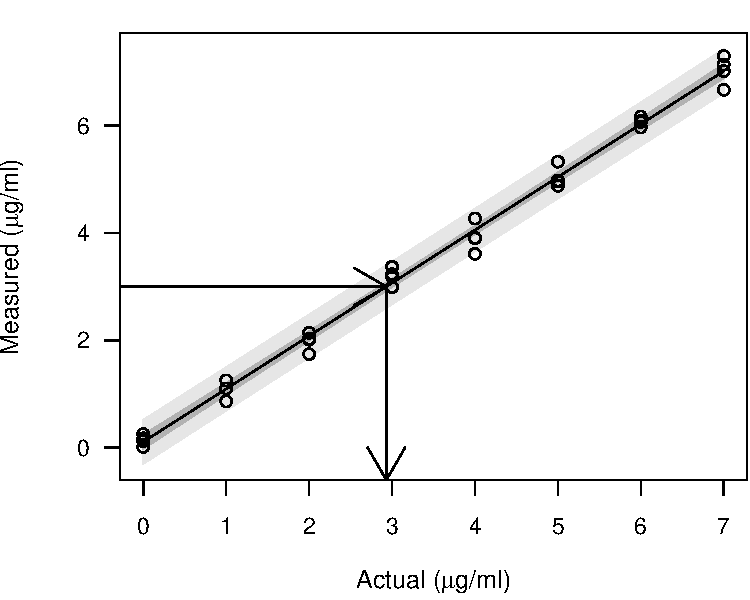
\includegraphics[width=\maxwidth]{figure/arsenic-fit} \caption[Fitted calibration line for the arsenic data]{Fitted calibration line for the arsenic data. The horizontal arrow indicates the position of the observed response $y_0 = 3$ $\mu$g/ml and the vertical arrow indicates the position of the \ac{ML} estimate $\wh{x}_0 = 2.941$.\label{fig:arsenic-fit}}
\end{figure}


\end{knitrout}


\section{Confidence intervals}
\label{sec:interval-estimation}
Much effort has been put into deriving and comparing point estimators for $x_0$. Without some measure of precision, however, a point estimate is practically useless. In this section, we discuss construction of $100(1-\alpha)\%$ confidence intervals for $x_0$, also known as \textit{calibration intervals}. There are two methods commonly used for calculating calibration intervals \citep{zeng_bootstrap_1997}: \textit{inversion intervals} and \textit{Wald intervals}, additionally, we also discuss bootstrap calibration intervals. A discussion on Bayesian credible intervals is deferred until Section~\ref{sec:bayesian}. For the most part, we assume the regression model \eqref{eqn:nonlinear-model} with normal errors and constant variance is appropriate and that the predictor values are fixed by design. 

%% Inversion interval
\subsection{Inversion interval}
\label{sec:inversion-interval}
Similar to inverting the calibration curve to obtain a point estimate, a confidence interval for $x_0$ can be constructed by inverting a prediction interval for the response. We refer to this type of calibration interval as the inversion interval. The inversion interval relies on the distribution of the \textit{predictive pivot}, $\mc{Q}$, which for the linear calibration problem is given by
\begin{equation}
\label{eqn:predictive-pivot}
  \mc{Q} = \frac{\wb{\mc{Y}}_0-\wh{\beta}_0-\wh{\beta}_1 x_0}{\sqrt{\wh{\sigma}_\epsilon^2\left[\frac{1}{m}+\frac{1}{n}+\frac{(x_0-\bar{x})^2}{S_{xx}}\right]}}.
\end{equation}
It can be shown \citep{graybill_theory_1976} that $\mc{Q} \sim \mathcal{T}\left(n+m-3\right)$, hence, 
\begin{equation*}
  \Prob\left(\tquant{\alpha/2}{n+m-3} < \mc{Q} < \tquant{1-\alpha/2}{n+m-3}\right) = 1-\alpha.
\end{equation*}
Squaring both sides of the inequality and expanding, we obtain a simple quadratic in $x_0$:
\begin{equation}
\label{eqn:quadratic}
  \Prob\left( a x_0^2 + b x_0 + c < 0 \right) = 1 - \alpha,
\end{equation}
where 
\begin{align*}
  a &= \wh{\beta}_1^2-\wh{\sigma}_\epsilon^2 t^2/S_{xx} \\
  b &= 2\left[\frac{\bar{x}\wh{\sigma}_\epsilon^2 t^2}{S_{xx}}-\wh{\beta}_1\left(\wb{\mc{Y}}_0-\wb{\mc{Y}}\right)-\wh{\beta}_1^2\bar{x}\right] \\
  c &= \left[\left(\wb{\mc{Y}}_0-\wh{\beta}_0\right)^2-\wh{\sigma}_\epsilon^2 t^2\left(\frac{1}{m}+\frac{1}{n}+\frac{\bar{x}^2}{S_{xx}}\right)\right] \\
  t &= \tquant{1-\alpha/2}{n+m-3}.
\end{align*}
An exact $100(1 - \alpha)\%$ confidence interval for $x_0$ is given by the set
\begin{equation}
\label{eqn:quadratic-inequality}
  \mathcal{J}_\mathrm{cal}\left(x\right) = \left\{x: a x^2 + b x + c < 0 \right\}.
\end{equation}
Although we use the term confidence \emph{interval} here, it is possible that the values of $x$ that satisfy this inequality do not form an actual interval. In particular, four possibilities exist: 
\begin{enumerate}[(i)]
  \item the set is a finite interval, $\mathcal{J}_\mathrm{cal}\left(x\right) = (L, U)$; 
  \item the set is the entire real line, $\mathcal{J}_\mathrm{cal}\left(x\right) = (-\infty, \infty)$; 
  \item the set consists of two semi-infinite intervals, $\mathcal{J}_\mathrm{cal}\left(x\right) = (-\infty, U) \cup (L, \infty)$; 
  \item the set is empty, $\mathcal{J}_\mathrm{cal}\left(x\right) = \emptyset$. 
\end{enumerate}
The circumstances leading to (i)-(iv) are depicted in Figure~\ref{fig:quadratics}. A finite interval (i) will occur if and only if $a > 0$ and $b^2 - 4ac > 0$. Upon closer inspection of the quadratic in Equation~\eqref{eqn:quadratic}, we see that this occurs when $a > 0$ or rather when $\wh{\beta}_1^2/(\wh{\sigma}_\epsilon^2/S_{xx}) > t^2$. In other words, when the slope $\wh{\beta}_1$ is significantly different from zero at the specified $\alpha$ level (i.e., the regression line is not too flat), the solution to Equation~\eqref{eqn:quadratic-inequality} forms a $100(1-\alpha)\%$ confidence interval for $x_0$ and is given by
\begin{equation}
\label{eqn:x0_ci_inv}
  \bar{x} + \frac{\wh{\beta}_1(\bar{y}_0-\bar{y})}{a} \pm \frac{t\wh{\sigma}}{a} \times \sqrt{a\left(\frac{1}{m}+\frac{1}{n}\right) + \frac{(\bar{y}_0-\bar{y})^2}{S_{xx}}}.
\end{equation}
or equivalently
\begin{equation*}
  \wh{x}_0 + \frac{(\wh{x}_0-\bar{x})g \pm \left(t\wh{\sigma}/\wh{\beta}_1\right)\sqrt{(\wh{x}_0-\bar{x})^2/S_{xx} + (1-g)\left(\frac{1}{m}+\frac{1}{n}\right)}}{1-g},
\end{equation*}
where $g = \left(t^2\wh{\sigma}_\epsilon^2\right)/(\wh{\beta}_1^2 S_{xx})$. The dependence on a statistically significant slope is generally not regarded as a concern since ``any self-respecting calibrator will design a calibration experiment such that his or her instrument is expected to have a statistically significant slope ...'' \citep[pp. 25]{brown_measurement_1993}. \citet{hoadley_bayesian_1970} noted that the width of interval \eqref{eqn:x0_ci_inv} depends on the value of the observed test statistic, $\mc{F}^\boot = \wh{\beta}_1^2S_{xx}/\wh{\sigma}_\epsilon^2 = t^2$, for testing $\mc{H}_0: \beta_1 = 0$ versus $\mc{H}_1: \beta_1 \ne 0$. A large value of $\mc{F}^\boot$ is associated with a smaller interval and vice versa. An approximation can be obtained by setting $g = 0$ in Equation~\eqref{eqn:x0_ci_inv}, which gives
\begin{equation}
\label{eqn:x0_ci_inv_approx}
  \wh{x}_0 \pm \tquant{1-\alpha/2}{n+m-3}\left(\frac{\wh{\sigma}}{\wh{\beta}_1}\right)^2\sqrt{\frac{1}{m}+\frac{1}{n}+\frac{(\wh{x}_0-\bar{x})^2}{S_{xx}}}.
\end{equation}
This approximation is useful when $g$ is small, say $g < 0.05$ \citep{draper_applied_1981}. Fieller's method \citep{fieller_some_1954}, which applies to the ratio of normally distributed random variables, can also be used to derive interval \eqref{eqn:x0_ci_inv} using a fiducial argument. Extending the inversion interval to the case of multiple predictors is discussed in \citet[pg. 229]{draper_applied_1981} and in \citet[chap. 3]{brown_measurement_1993}. Brown considers the special case of polynomial regression.

\begin{knitrout}
\definecolor{shadecolor}{rgb}{0.969, 0.969, 0.969}\color{fgcolor}\begin{figure}[H]

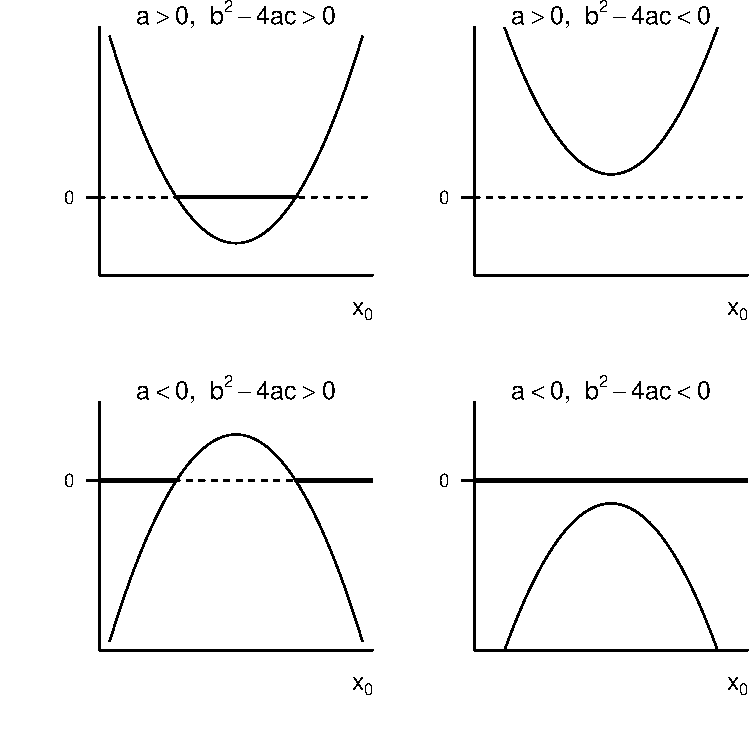
\includegraphics[width=\maxwidth]{figure/quadratics} \caption[Solutions to the equation $ax^2 + bx + c < 0$]{Solutions to the equation $ax^2 + bx + c < 0$. \textit{Top left}: The set is an interval. \textit{Top right}: The set is empty. \textit{Bottom left}: The set consists of two semi-infinite intervals. \textit{Bottom right}: The set is the entire real line.\label{fig:quadratics}}
\end{figure}


\end{knitrout}


For nonlinear calibration curves, 
\begin{equation}
\label{eqn:approximate-predictive-pivot}
  \mc{Q} = \frac{\wb{\mc{Y}}_0 - \mu\left(x_0; \wh{\bm{\beta}}\right)}{\sqrt{\wh{\sigma}_\epsilon^2/m + \wh{\var}\left\{\mu\left(x_0; \wh{\bm{\beta}}\right)\right\}}}
\end{equation}
is only an approximate pivot. We assume $\mc{Q} \sim \mc{N}(0, 1)$ as $n$ goes to $\infty$. An approximate $100(1 - \alpha)\%$ confidence interval for $x_0$ based on Equation~\eqref{eqn:approximate-predictive-pivot} is the set 
\begin{equation}
\label{eqn:nonlinear-inversion-interval}
  \wh{\mc{J}}_\mathrm{cal}(x) = \left\{x: z_{\alpha/2} < \frac{\bar{y}_0 - \mu\left(x; \wh{\bm{\beta}}\right)}{\sqrt{\wh{\sigma}_\epsilon^2/m + \wh{\var}\left\{\mu\left(x; \wh{\bm{\beta}}\right)\right\}}} < z_{1-\alpha/2} \right\},
\end{equation}
where $z_{\alpha/2}$ and $z_{1-\alpha/2}$ are the $\alpha/2$ and $1-\alpha/2$ quantiles of the standard normal distribution, respectively. To be more conservative, we can replace the normal quantiles with those of a $\mathcal{T}\left(n+m-p-1\right)$ distribution ($p$ being the dimension $\bm{\beta}$). Unlike the linear calibration problem, the solution to Equation~\eqref{eqn:nonlinear-inversion-interval} cannot be written in closed-form and will require iterative techniques. 

For the special case $m = 1$, the inversion interval is equivalent to drawing a horizontal line through the scatterplot of the standards at $y_0$ and finding the abscissas of its intersection with the $100(1-\alpha)\%$ (pointwise) prediction band of the calibration curve. For the straight line case, if $\beta_1$ is not significantly different from zero, the regression line is not well determined and the horizontal line drawn at $y_0$ will not intersect the prediction band at two points, leading to cases (ii) or (iii) outlined above; this point is illustrated in Figure~\ref{fig:bands}. The issue in linear calibration is that prediction bands are really hyperbolas which, depending on the quality of the model/data, can bend quite severely. To circumvent this problem, \citet{trout_regular_1979} proposed a similar procedure based on uniform prediction bands (i.e., prediction bands that are parallel to the calibration line). This has the advantage of always producing a (symmetric) confidence interval for $x_0$, without sacrificing efficiency. 

\begin{knitrout}
\definecolor{shadecolor}{rgb}{0.969, 0.969, 0.969}\color{fgcolor}\begin{figure}[H]

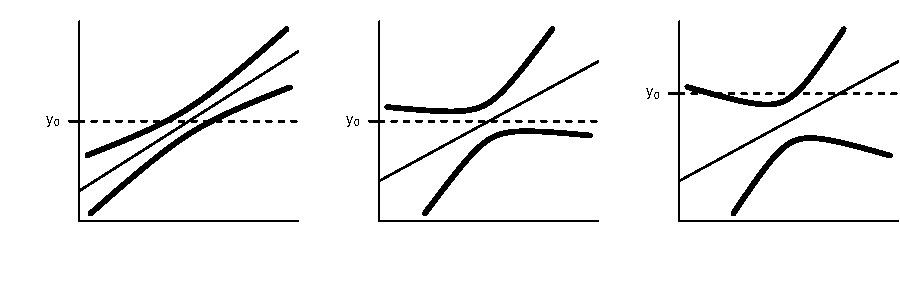
\includegraphics[width=\maxwidth]{figure/bands} \caption[Common prediction band shapes]{Common prediction band shapes. \textit{Left}: Horizontal line at $y_0$ intersects the prediction band at two points, resulting in a finite interval. \textit{Middle}: Horizontal line at $y_0$ does not intersect the prediction band at all resulting in an infinite interval. \textit{Right}: Horizontal line at $y_0$ only intersects with one side of the prediction band resulting in two semi-infinite intervals.\label{fig:bands}}
\end{figure}


\end{knitrout}


Similarly, we can compute the inversion interval for nonlinear calibration problems by drawing the prediction band, however, inference in nonlinear regression often relies on linear approximations, large samples, and approximate normality. For nonlinear calibration curves, the bootstrap (see Section~\ref{sec:boot_int}) may provide more accurate results. Drawing the prediction band for calibration curves also gives an idea as to what values of $y_0$ lead to meaningful interval estimates for $x_0$. For example, an observed value $y_0$ too close to a horizontal asymptote will produce a useless confidence interval for $x_0$ (if at all). Graphical methods like this are discussed by \citet{jones_approximate_2009} who extend the approach for longitudinal data with bivariate response.

%% Wald interval
\subsection{Wald interval}
\label{sec:wald_int}
Another common approach for obtaining a confidence interval for the unknown $x_0$ is to use the delta method \citep{verhoef_who_2012, dorfman_note_1938}, also see \citet{casella_statistical_2002}. Let the variance-covariance matrix of $\left(\wb{\mc{Y}}_0, \wh{\bm{\beta}}\right)\trans$ be given by $\bm{\Sigma}$ where
\begin{equation*}
  \bm{\Sigma} = 
    \begin{bmatrix}
      \var\left\{\wb{\mc{Y}}_0\right\} & \cov\left\{\wb{\mc{Y}}_0, \wh{\bm{\beta}}\right\} \\
      \cov\left\{\wb{\mc{Y}}_0, \wh{\bm{\beta}}\right\} & \var\left\{\wh{\bm{\beta}}\right\}
    \end{bmatrix}.
\end{equation*}
Recall that $\wh{\bm{\beta}}$ is a linear function of the observations $\bc{Y}$. Since $\wb{\mc{Y}}_0$ is independent of $\bc{Y}$, it follows that $\wb{\mc{Y}}_0$ and $\wh{\bm{\beta}}$ are also independent; hence, $\cov\left\{\wb{\mc{Y}}_0, \wh{\bm{\beta}}\right\} = \bm{0}_{p \times p}$. Therefore, $\bm{\Sigma}$ simplifies to
\begin{equation*}
  \bm{\Sigma} = 
    \begin{bmatrix}
      \sigma_\epsilon^2/m & \bm{0}_{p \times p} \\
      \bm{0}_{p \times p} & \sigma_\epsilon^2\left(\X\trans\X\right)^{-1}
    \end{bmatrix}.
\end{equation*}
The classical estimator, $\wh{x}_0$, has the form $x = \mu^{-1}\left(y; \bm{\beta}\right)$. Let $\mu_1^{-1}\left(y; \bm{\beta}\right) = \frac{\partial}{\partial y}\mu^{-1}\left(y; \bm{\beta}\right)$ and $\mu_2^{-1}\left(y; \bm{\beta}\right) = \frac{\partial}{\partial \bm{\beta}}\mu^{-1}\left(y; \bm{\beta}\right)$. Note that if $p$ (the dimension of $\bm{\beta}$) is greater than one, then $\mu_2^{-1}\left(y; \bm{\beta}\right)$ will be a vector valued function. The delta method estimate of the variance of $\wh{x}_0 = \mu^{-1}\left(\wb{\mc{Y}}_0; \wh{\bm{\beta}}\right)$, based on a first-order Taylor series expansion, is given by
\begin{equation}
  \label{eqn:x0-lm-delta}
  \wh{\var}\left\{\wh{x}_0\right\} = \frac{\wh{\sigma}_\epsilon^2}{m}\left[\mu_1^{-1}\left(\wb{\mc{Y}}_0; \wh{\bm{\beta}}\right)\right]^2 + \wh{\sigma}_\epsilon^2\left[\mu_2^{-1}\left(\wb{\mc{Y}}_0; \wh{\bm{\beta}}\right)\right]\trans\left(\X\trans\X\right)^{-1}\left[\mu_2^{-1}\left(\wb{\mc{Y}}_0; \wh{\bm{\beta}}\right)\right].
\end{equation}
For the simple linear calibration problem, Equation~\eqref{eqn:x0-lm-delta} reduces to
\begin{equation*}
  \wh{\var}\left\{\wh{x}_0\right\} = \frac{\wh{\sigma}_\epsilon^2}{\wh{\beta}_1^2}\left[\frac{1}{m}+\frac{1}{n}+\frac{(\wh{x}_0-\bar{x})^2}{S_{xx}}\right]. 
\end{equation*}
The estimated standard error ($\se$) of $\wh{x}_0$ is just $\se\left\{\wh{x}_0\right\} = \sqrt{\wh{\var}\left\{\wh{x}_0\right\}}$.

Assuming that
\begin{equation}
\label{eqn:approx_pivot}
  \mc{W} = \frac{\wh{x}_0 - x_0}{\wh{\se}\left\{\wh{x}_0\right\}} \stackrel{\cdot}{\sim} \mc{N}(0, 1)
\end{equation}
for ``large'' $n$ leads to an approximate $100(1-\alpha)\%$ Wald-based confidence interval for $x_0$ of 
\begin{equation}
\label{eqn:x0_ci_wald}
  \wh{x}_0 \pm \tquant{1-\alpha/2}{n+m-p-1} \cdot \wh{\se}\left\{\wh{x}_0\right\},
\end{equation}
where $\tquant{1-\alpha/2}{n+m-p-1}$ is the $1-\alpha/2$ quantile of a Student's $t$-distribution with $n+m-p-1$ degrees of freedom. If the sample size is large enough, we could replace $t{1-\alpha/2}{n+m-p-1}$ with $z_{1-\alpha/2}$, the $1-\alpha/2$ quantile of a standard normal distribution. Unlike the inversion interval, Equation~\eqref{eqn:nonlinear-inversion-interval}, the Wald-based interval always exists and is symmetric about the point estimate $\wh{x}_0$. This approach is useful when it is difficult (or impossible) to invert a corresponding prediction interval. The symmetry of the Wald interval, however, may be unrealistic in nonlinear calibration problems when, for example, $\bar{y}_0$ is near a horizontal asymptote \citep{schwenke_callibration_1991}. Perhaps the biggest drawback is the approximate normality assumption for $\mc{W}$, which is not always reasonable in practice. For example, in simple linear calibration, the distribution of $\wh{x}_0$ may not even be unimodal \citep{buonaccorsi_design_1986}. On the other hand, for the simple linear calibration problem, the Wald-based interval is equivalent to the approximate inversion interval given in Equation~\eqref{eqn:x0_ci_inv_approx}. Thus, provided $g$ is ``small,'' the Wald interval may perform well even when $\mc{W}$ is not asymptotically normal.

\citet{schwenke_callibration_1991} discuss the inversion and Wald confidence intervals for nonlinear calibration. Using simulation, they showed that the inversion and Wald intervals can attain the desired confidence level in samples of size 20 for a nonlinear exponential decay model. They also discuss testing the equality of two calibration points. However, Schwenke and Millikem treat $\mc{Y}_0$ as a fixed constant. In regulation-type problems, this is the correct approach. However, in calibration, the confidence interval for $x_0$ will be too narrow. To illustrate, consider the conventional treatment group of the postmortem data analyzed in \citet{schwenke_callibration_1991}. In essence, Schwenke and Millikem computed the time corresponding to a mean pH level of 6.0, not an observed pH level of 6.0. They list a 95\% Wald-based confidence interval for $x_0$ of $(3.315, 4.317)$. Accounting for the correct variation, however, this interval should actually be $(2.615, 5.016)$. The standard error they computed for $\wh{x}_0$ is based on $\bm{T} = (\wh{\beta}_0, \wh{\beta}_1, \wh{\beta}_2)\trans$ whereas here it is based on $\bm{T} = (\mc{Y}_0, \wh{\beta}_0, \wh{\beta}_1, \wh{\beta}_2)\trans$. In short, Schwenke and Millikem only account for the variance of the estimated regression parameters whereas in a true calibration problem, the variance of $\mc{Y}_0$ needs to be taken into account. 

There is an interesting relationship in the linear calibration problem (with $m = 1$) between the Wald interval for $x_0$, interval~\eqref{eqn:x0_ci_wald}, and a prediction interval for $\mc{Y}_0$. Let $L_w$ and $U_w$ denote the lower and upper bounds, respectively, from a $100(1 - \alpha)\%$ Wald confidence interval for $x_0$ corresponding to an observed $y_0$. If $\wh{x}_0$ is assumed given, then it is easy to show that a $100(1 - \alpha)\%$ prediction interval for $\mc{Y}_0$ is $(\wh{\beta}_0+\wh{\beta}_1 L_w, \wh{\beta}_0+\wh{\beta}_1 U_w)$ if $\wh{\beta}_1 > 0$ and $(\wh{\beta}_0+\wh{\beta}_1 U_w, \wh{\beta}_0+\wh{\beta}_1 L_w)$ if $\wh{\beta}_1 < 0$. This relationship is illustrated in Figure~\ref{fig:arsenic-wald} for the arsenic example. %This method provides the researcher with a quick and simple way to calculate calibration intervals since most statistical software packages only provide prediction intervals.

\begin{knitrout}
\definecolor{shadecolor}{rgb}{0.969, 0.969, 0.969}\color{fgcolor}\begin{figure}[H]

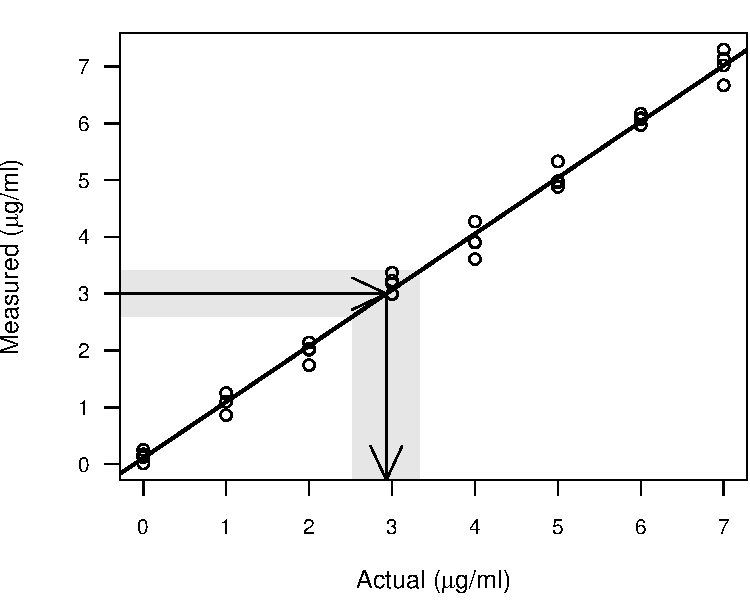
\includegraphics[width=\maxwidth]{figure/arsenic-wald} \caption[Relationship beween Wald interval for $x_0$ and prediction interval for $\mc{Y}_0$]{Scatterplot of the arsenic data with fitted calibration line. The horizontal arrow represents the response measurement for the new sample and the vertical arrow represents the \ac{ML} estimate of the unknown concentration. The vertical gray band represents a 95\% Wald confidence interval for $x_0$ corresponding to $y_0 = 3$ and the horizontal gray band represents a 95\% prediction interval for $\mc{Y}_0$ corresponding to $x_0 = \wh{x}_0$.\label{fig:arsenic-wald}}
\end{figure}


\end{knitrout}


%% Bootstrap intervals
\subsection{Bootstrap intervals}
\label{sec:boot_int}
In many applications, the calibration curve is usually nonlinear (e.g., dose-response curves and other types of assay data). Although the inversion and Wald procedures can still be applied, they can be highly inaccurate when the sample size is small. A useful alternative in these situations is to use the nonparametric bootstrap \citep{efron_bootstrap_1979}, which is a computer intensive technique based on sampling with replacement from the observed data. As such, the bootstrap provides an alternative means to computing bias, standard errors, and confidence intervals. Unlike the delta method, however, which is only first-order accurate, the bootstrap can often have ``second-order'' accuracy \citep[pg. 517]{casella_statistical_2002}. The bootstrap is not without assumptions (e.g., independent observations are still required), but it does allow us to relax the usual assumptions of large sample size and normality. The supporting mathematics can be quite involved, but the interested reader is pointed to \citet{efron_boot_1994} and \citet{hall_bootstrap_1992}. A detailed and practical guide to the bootstrap is given by \citet{davison_bootstrap_1997}. 

Let $\wh{\mu}_i = \mu\left(x_i; \wh{\bm{\beta}}\right)$ be the \textit{fitted values} and $\wh{\bm{\beta}}$ be the least squares estimate of $\bm{\beta}$. The two (nonparametric) bootstrap resampling schemes for regression are:
\begin{description}
  \item[case resampling:] pairs of data are sampled with replacement to produce \\ $\left(x_1, y_1\right)^\boot, \dotsc, \left(x_n, y_n\right)^\boot$;
  \item[model-based resampling:] the residuals $e_1, \dotsc, e_n$, or a modified version \\thereof, are sampled with replacement and added to the fitted values to produce $\left(x_1, \wh{\mu}_1+e_1^\boot\right), \dotsc, \left(x_n, \wh{\mu}_n+e_n^\boot\right)$.
\end{description}
\citet{efron_boot_1994} and \citet{davison_bootstrap_1997} discuss the merits of both schemes. Model-based resampling is more appropriate when the values of the independent variable are fixed by design (e.g., controlled calibration experiments) and the errors have constant variance. Resampling cases, on the other hand, is less accurate but more robust to violations of the model assumptions such as homoscedastistic errors. 

Various bootstrap approaches to calibration have been suggested in the literature. \citet{rosen_constructing_1995} discuss controlled calibration based on a parametric bootstrap where, instead of sampling directly from the residuals, samples are drawn from a normal distribution. This procedure will work even when the calibration curve is estimated nonparametrically (e.g., \textit{cubic smoothing splines}). \citet{zeng_bootstrap-adjusted_1997} commented that the procedure proposed by Rosen and Cohen requires a large number of resamples to achieve the desired accuracy. They suggested a bootstrap adjustment to the inversion and Wald intervals that requires far fewer bootstrap resamples. Given the speed and multicore functionality of modern computers, a large number of resamples, say 10,000 or more, is less of a concern. 

In this section, we outline a general bootstrap approach to controlled calibration in Algorithm~\ref{alg:boot_cal}, but first we discuss a rather naive approach. For an observed $\bar{y}_0$, suppose we compute $R$ bootstrap replicates of $\wh{x}_0$, and then use, for example, the sample $\alpha/2$ and $1 - \alpha/2$ quantiles as a $100(1 - \alpha)\%$ confidence interval for $x_0$. This results in $\bar{y}_0$ being treated as a fixed parameter in the bootstrap simulation, but in fact, $\bar{y}_0$ is an observed value of the random variable $\wb{\mc{Y}}_0$ which has variance $\sigma_\epsilon^2/m$. In other words, some variation is not getting accounted for in this approach. This is akin to ignoring $\var\left\{\wb{\mc{Y}}_0\right\}$ in the delta method discussed previously. One solution is to simulate the correct variance by adding a small amount of noise to the observed responses from the second stage of the calibration experiment.

\begin{algorithm}[!htb]
\begin{singlespace}
\SetAlgoNoLine
\For{$r = 1$ \KwTo $R$}{
\begin{enumerate}[(1)]
  \item \For{$i = 1$ \KwTo $n$}{
	  \begin{enumerate}[(a)]
      \item set $x_i^\boot = x_i$\;
	    \item randomly sample $\epsilon_i^\boot$ from the centered residuals $e_1', \dotsc, e_n'$\;
	    \item set $y_i^\boot = \mu\left(x_i; \wh{\bm{\beta}}\right) + \epsilon_i^\boot$\;
		\end{enumerate}
  }
	\item Fit model to $\left(x_1^\boot, y_1^\boot\right), \dotsc, \left(x_n^\boot, y_n^\boot\right)$, giving estimates $\wh{\bm{\beta}}_r^\boot$, $\wh{\sigma}_r^{2\boot}$\;
	\item \For{$j = 1$ \KwTo $m$}{
	  \begin{enumerate}
		  \item randomly sample $\epsilon_j^\boot$ from the centered residuals $e_1', \dotsc, e_n'$\;
			\item set $y_{0j}^\boot = \bar{y}_0 + \epsilon_j^\boot$\;
		\end{enumerate}
	}
	\item Set $\bar{y}_{0r}^\boot = \sum_{k=1}^m y_{0k}^\boot/m$\;
	\item Set $\wh{x}_{0r}^\boot = \mu^{-1}\left(\bar{y}_{0r}^\boot; \wh{\bm{\beta}}_r^\boot\right)$\;
\end{enumerate}
\vspace{5pt}
\textit{if calculating an interval based on the studentized bootstrap, then additionally:}
\vspace{5pt}
\begin{enumerate}[(1)]
  \setcounter{enumi}{5}
	\item Compute $\wh{\se}\left\{\wh{x}_{0r}^\boot\right\}$\;
	\item Set $\mc{W}_r^\boot = (\wh{x}_{0r}^\boot - \wh{x}_0) / \wh{\se}\left\{\wh{x}_{0r}^\boot\right\}$\;
\end{enumerate}
}
\end{singlespace}
\caption{Model-based resampling for controlled calibration. \label{alg:boot_cal}}
\end{algorithm}

A few issues regarding the residuals in Algorithm~\ref{alg:boot_cal} are worth considering. For the linear case, it is preferable to scale the residuals before centering \citep{davison_bootstrap_1997}. In particular, compute $r_i = e_i/\sqrt{1-h_{ii}}$, where $h_{ii}$ are the diagonal elements of the hat matrix, $\bm{H} = \X\trans(\X\trans\X)^{-1}\X$. We then sample $\epsilon_j^\boot$ from the modified residuals $r_1 - \bar{r}, \dotsc, r_n - \bar{r}$. This transforms the residuals so that they are centered and have constant variance $\sigma_\epsilon^2$. For nonlinear calibration curves, the residuals should be corrected for bias in addition to centering them \citep{davison_bootstrap_1997}. When there are outliers in the residuals, the bootstrap distribution of $\wh{x}_0$ can become skewed or multimodal. One suggestion is to replace the residuals in step (3) with something smoother, say random variates from a normal distribution. For the case $m > 1$, \citet{jones_bootstrapping_1999} suggest using a ``residual pool'' formed by $e_1, \dotsc, e_n$ plus residuals computed from the unknowns: $e_{n+j} = y_{n+j} - \bar{y}_0$ $(j = 1, 2, \dotsc, m)$. In Section~\ref{sec:point-estimation}, we mentioned that it is often reasonable to assume $\sigma_{\text{I}}^2 = \sigma_{\text{II}}^2$. However, if this assumption is not valid, then we can still proceed by resampling separately from the two sets of residuals $\big\{e_i\big\}_{i = 1}^n$ and $\big\{e_j\big\}_{j = n + 1}^{n + m}$ \citep{gruet_calibration_1993, jones_bootstrapping_1999}. For instance, we can resample from $\big\{e_i\big\}_{i = 1}^n$ in step (1) and from $\big\{e_j\big\}_{j = n + 1}^{n + m}$ in step (3) of Algorithm~\ref{alg:boot_cal}. We can also accommodate nonconstant variance (i.e., heteroscedasticity) by applying the \textit{wild bootstrap} \citep[pp. 272]{davison_bootstrap_1997}. This approach is discussed in \citet[pp. 142]{huet_statistical_2004}.

Once we have our bootstrap replicates, a number of different bootstrap confidence intervals can be constructed. For a studentized interval, we compute $R$ bootstrap replicates of $\mc{W}$ (Equation~\eqref{eqn:approx_pivot}): $\mc{W}_1^\boot, \mc{W}_2^\boot, \dotsc, \mc{W}_R^\boot$. This is outlined in steps (6)-(7) of Algorithm~\ref{alg:boot_cal}. Instead of relying on normal theory assumptions about $\mc{W}$, as when computing the Wald interval, the bootstrap estimates the distribution of $\mc{W}$ directly from the data. Thus, instead of approximating the quantiles of $\mc{W}$ using a standard table, a ``table is built for the data at hand'' \citep{efron_boot_1994}. An approximate $100(1 - \alpha)\%$ confidence interval for $x_0$ based on the studentized bootstrap is given by
\begin{equation}
\label{eqn:student_int}
  \left( \wh{x}_0 - \gamma_{1-\alpha/2}^\boot \cdot \wh{\se}\left\{\wh{x}_0\right\}, \wh{x}_0 - \gamma_{\alpha/2}^\boot \cdot \wh{\se}\left\{\wh{x}_0\right\} \right),
\end{equation}
where $\gamma_{\alpha/2}^\boot$ and $\gamma_{1 - \alpha/2}^\boot$ are the sample quantiles from the bootstrap distribution of $\mc{W}$. One drawback of this approach is that it requires an estimate of the standard error, $\wh{\se}\left\{\wh{x}_{0r}^\boot\right\}$. We could use a Taylor series approximation, as in the delta method, but this is known to be unreliable for small samples. Another alternative is to use the bootstrap to estimate the standard error of each $\wh{x}_{0r}^\boot$. This implies a second level of bootstrapping nested within the first and can be computationally expensive. The studentized interval for controlled calibration using the large-sample formula for the standard error (see Equation~\eqref{eqn:x0-lm-delta}) is discussed by \citet{zeng_bootstrap-adjusted_1997} and  \citet{jones_bootstrapping_1999}. This interval can perform poorly in practice and is easily influenced by outliers in the data. 

Yet another technique \citep{jones_bootstrapping_1999, huet_statistical_2004} is to bootstrap the predictive pivot in Equation~\eqref{eqn:approximate-predictive-pivot}:
\begin{equation*}
  \mc{Q}^{\boot} = \frac{\bar{y}_0^\boot - \mu\left(\wh{x}_0; \wh{\bm{\beta}}^\boot\right)}{\wh{\se}^\boot\left\{\bar{y}_0^\boot - \mu\left(\wh{x}_0; \wh{\bm{\beta}}^\boot\right)\right\}} = \frac{\bar{y}_0^\boot - \mu\left(\wh{x}_0; \wh{\bm{\beta}}^\boot\right)}{\sqrt{\wh{\sigma}_\epsilon^{2\boot}/m + \wh{\var}^\boot\left\{\mu\left(\wh{x}_0; \wh{\bm{\beta}}^\boot\right)\right\}}}.
\end{equation*}
It is is easy to see that, for the linear calibration problem, $\mc{Q}^\boot = \mc{W}^\boot$; therefore, the resulting interval is the same. For the nonlinear calibration problem, however, a $100(1-\alpha)\%$ confidence interval for $x_0$ based on the bootstrapping the predictive pivot is given by the set
\begin{equation*}
	\mc{J}_\mathrm{cal}^\boot(x) = \left\{x: q_{\alpha/2}^\boot \le \mc{Q} \le q_{1-\alpha/2}^\boot\right\},
\end{equation*}
where $q_{\alpha/2}^\boot$ and $q_{1-\alpha/2}^\boot$ are the $\alpha/2$ and $1-\alpha/2$ quantiles of the bootstrap distribution of $\mc{Q}$, respectively. This mimics the inversion method discussed in Section~\ref{sec:inversion-interval} but usually performs better since we no longer have to rely on the approximate normality of $\mc{Q}$. Therefore, we might think of this as a bootstrap adjusted inversion interval. According to \citet{huet_statistical_2004}, this procedure performs reasonably well in practice, even with small sample sizes and $R$ as small as 200.

On the other hand, we can avoid computing a pivot altogether by working directly with the bootstrap replicates of $\wh{x}_0$ from step (5) of Algorithm~\ref{alg:boot_cal}. A simple and often satisfactory procedure, known as the percentile bootstrap, uses the sample $\alpha/2$ and $1 - \alpha/2$ quantiles of $\wh{x}_{01}^\boot, \dotsc, \wh{x}_{0R}^\boot$ as a confidence interval for $x_0$. A more accurate technique is the \textit{bias-corrected and accelerated} ($BC_a$) interval, which is essentially a modification of the percentile interval; for details see \citet[chap. 14, sec. 3]{efron_boot_1994}. The $BC_a$ method tends to work well, but usually requires $R$ to be large. It is both second-order accurate \citep[pp. 187]{efron_boot_1994} and transformation respecting. For example, if we want a $BC_a$ confidence interval for $\log(x_0)$, we can simply log the endpoints of the corresponding $BC_a$ interval for $x_0$. The studentized interval is also second-order accurate, but not transformation respecting, while the percentile interval is transformation respecting but only first-order accurate. For an in-depth discussion regarding the different bootstrap confidence interval procedures, see \citet[chap. 5]{davison_bootstrap_1997}.

A related method for computing calibration intervals, based on the \textit{jackknife}, was given by \citet{miller_unbalanced_1974}. Let $\beta = h(\bm{\beta})$ be a function of the regression parameters. Miller showed that, under reasonable conditions, the jackknife estimate
\begin{equation*}
  \wh{\beta}_\text{jack} = n\wh{\beta} - \frac{n-1}{n}\sum_{i=1}^n\wh{\beta}_{(-i)},
\end{equation*}
where $\wh{\beta}_{(-i)}$ denotes the estimate of $\beta$ with the $i$-th observation removed from the data, is asymptotically normally distributed (even if the errors $\epsilon_i$ are not normally distributed). Hence, an approximate $100(1-\alpha)\%$ confidence interval for $x_0$ can be developed that does not require a normality assumption for the errors of the model. However, $x_0$ is not just a function of $\bm{\beta}$, but also of $\wb{\mc{Y}}_0$. This is not a problem as long as $m > 1$ and $m/n \rightarrow c$, $0 < c < \infty$. For regulation \citep[pp. 431-432]{graybill_regression_1994}, $x_0$ is a function of the regression parameters only; hence, the jackknife-based interval is easily applied.

%% Bayesian calibration
\section{Bayesian calibration}
\label{sec:bayesian}
Although calibration has been the subject of much discussion and debate from a frequentist point of view, it is just as intriguing from a Bayesian perspective. Let $\bm{y}$, $\bm{y}_0$, and $\mathbf{data}$ represent the data from the standards, unknowns, and both, respectively. Also, if $x$ has a nonstandardized $t$-distribution with mean $\mu$, precision $\tau$ (i.e., recipricol of the variance), and $k$ degrees of freedom---denoted $x \sim \mathcal{T}_k(\mu, \tau)$---then the probability density function of $x$ is
\begin{equation*}
  f(x;\mu, \tau, k) = \frac{\Gamma{(k/2+1/2)}}{\Gamma{(k/2)}\sqrt{\tau k \pi}}\left[ 1 + \frac{(x-\mu)^2}{\tau k} \right]^{-(k+1)/2},
\end{equation*}
for $-\infty < x < \infty$, $-\infty < \mu < \infty$, $\tau > 0$, and $k \ge 1$.

Two influential papers on Bayesian calibration are \citet{hoadley_bayesian_1970} and \citet{hunter_bayesian_1981}. \citet[chap. 10]{aitchison_statistical_1980} discuss Bayesian solutions to the linear calibration problem for both natural and controlled calibration experiments. They also briefly discuss calibration under a general utility structure. \citet{dunsmore_bayesian_1967} derived the inverse estimator \eqref{eqn:x0-inverse} as the conditional mean of $x_0|\mathbf{data}$ assuming independent observations from a bivariate normal distribution (i.e., Gaussian data from a natural calibration experiment). For controlled calibration experiments, \citet{hoadley_bayesian_1970} argued that the classical estimator is unsatisfactory, since the width of the inversion interval \eqref{eqn:x0_ci_inv} depends on the magnitude of the F-statistic for testing the significance of the slope; in other words, the data contain information about the precision of $\wh{x}_0$. Because of this, Hoadley argues that less weight should be given to this estimator when it is known to be unreliable, which is what a Bayes estimator does. He proposed a class of Bayesian solutions assuming, \textit{a priori}, that $x_0$ is independent of $(\beta_0, \beta_1, \sigma_\epsilon^2)$. His results are based on a general prior of the form 
\begin{equation*}
  \pi\left(\beta_0, \beta_1, \sigma_\epsilon^2, x_0\right) = \pi\left(\beta_0, \beta_1, \sigma_\epsilon^2\right) \pi\left(x_0\right), 
\end{equation*}
but he obtained explicit results for the diffuse prior $\pi\left(\beta_0, \beta_1, \sigma_\epsilon^2\right) \propto 1/\sigma_\epsilon^2$. For the case $m=1$, he was able to derive the inverse estimator \eqref{eqn:x0-inverse} as a Bayes estimator under squared error loss with respect to a nonstandardized Student's $t$ prior distribution for $x_0$:
\begin{equation}
\label{eqn:x0prior}
  x_0 \sim \mathcal{T}_{n-3}\left\{\bar{x}, \left(1+\frac{1}{n}\right)\frac{S_{xx}}{n-3}\right\}. 
\end{equation}
This leads to the very simple result
\begin{equation}
\label{eqn:x0post}
  x_0|\mathbf{data} \sim \mathcal{T}_{n-2}\left\{\wt{x}_0, \frac{\wh{\sigma}_\epsilon^2 S_{xx}}{S_{yy}}\left( 1+\frac{1}{n}+\frac{(y_0 - \bar{y})^2}{S_{yy}} \right)\right\}. 
\end{equation}
A $100(1-\alpha)\%$ shortest credible interval for $x_0$ can be obtained from \eqref{eqn:x0post} and is given by
\begin{equation}
\label{eqn:sci}
  \wt{x}_0 \pm \sqrt{\frac{\wh{\sigma}_\epsilon^2 S_{xx}}{S_{yy}}\left( 1+\frac{1}{n}+\frac{(y_0 - \bar{y})^2}{S_{yy}} \right)F_{1-\alpha, 1, n-2}}.
\end{equation}

Although this provides some theoretical justification for using the inverse estimator in controlled calibration, Hoadley is aware that it is merely a by-product of the Bayesian approach and recommends a careful elicitation of prior information. \citet[pp. 198, 204]{aitchison_statistical_1980} give extensions of distributions \eqref{eqn:x0prior}-\eqref{eqn:x0post} and interval \eqref{eqn:sci} for the case $m > 1$. As they point out, this extension is somewhat nonsensical since the prior variance of $x_0$ depends on $m$, the number of future replicates. This is rather unrealistic, but ``... tractability in these calibration problems can lead to an unnecessary departure from reality ...'' \citep[pp. 198]{aitchison_statistical_1980}. Though many authors have criticized the classical estimator on the grounds that it has infinite MSE, Hoadley also contested its use based on the inherent problems of the inversion interval \eqref{eqn:quadratic}. These difficulties, however, do not arise with the shortest credible interval \eqref{eqn:sci}. Figure~\ref{fig:arsenic-bayes} shows the prior and posterior distributions of $x_0$ for the arsenic example (Section~\ref{sec:example_arsenic}) using Hoadley's approach. The mean of the posterior is $2.945$ $\mu$g/ml, the same as the inverse estimator, and the corresponding 95\% shortest credible interval for $x_0$ is $(2.547, 3.342)$.  

\begin{knitrout}
\definecolor{shadecolor}{rgb}{0.969, 0.969, 0.969}\color{fgcolor}\begin{figure}[H]

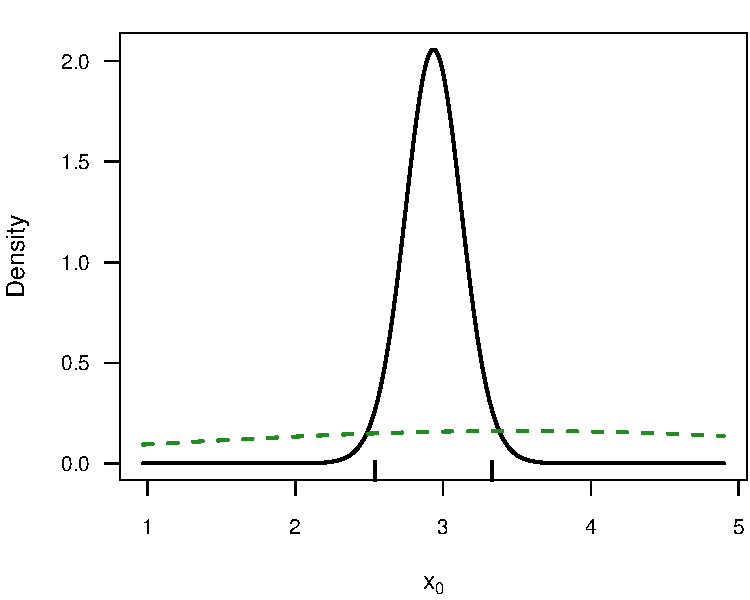
\includegraphics[width=\maxwidth]{figure/arsenic-bayes} \caption[Bayesian calibration for the arsenic example]{Bayesian calibration for the arsenic example. The black and green lines represent the posterior and prior for $x_0$, respectively. The posterior is symmetric and centered at $\wt{x}_0 = 2.945$. The tick marks indicate the endpoints of a 95\% HPD interval for $x_0$.\label{fig:arsenic-bayes}}
\end{figure}


\end{knitrout}


\citet{hunter_bayesian_1981} also considered the linear calibration problem, but proposed a slightly different approach. Let $\eta = \beta_0 + \beta_1 x_0$ and assume,\textit{a priori}, that $\eta$ and $(\beta_0, \beta_1, \sigma_\epsilon^2)$ are independent. Assuming normal errors, a prior for the unknown $x_0 = (\eta - \beta_0)/\beta_1$ is induced by specifying improper reference priors for $\eta$, $\beta_0$, $\beta_1$, and $\sigma_\epsilon^2$. That is, assuming 
\begin{equation*}
  \pi\left(\eta, \beta_0, \beta_1, \sigma_\epsilon^2\right) = \pi\left(\beta_0, \beta_1, \sigma_\epsilon^2\right) \pi\left(\eta\right) \propto 1/\sigma_\epsilon^2. 
\end{equation*}
This is quite different from the approach put forth by \citet{hoadley_bayesian_1970} who does not treat $x_0$ as an explicit function of $\eta$, $\beta_0$, and $\beta_1$. Hunter and Lamboy also discuss the case where $\sigma_\epsilon^2$ is known, or at least, assumed known. The posterior they obtain for $x_0$ is equivalent to the posterior density for the ratio of bivariate normal random variables ($\sigma_\epsilon^2$ known) or bivariate $t$ random variables ($\sigma_\epsilon^2$ unknown), both of which have infinite variance. The latter is actually a generalization of the structural distribution for $x_0$ obtained by \citet{kalotay_structural_1971}. A more thorough analysis of these posteriors is given by \citet{hunter_bayesian_1979} and \citet{hunter_making_1979}. Hunter and Lamboy claim that, under reasonable conditions, the inversion and Wald intervals (Section~\ref{sec:inversion-interval} and Section~\ref{sec:wald_int}) provide accurate approximations to the highest posterior density (HPD) region for $x_0$. That said, \citet{hill_discussion_1981}, \citet{orban_discussion_1981}, \citet{lwin_discussion_1981}, and \citet{brown_multivariate_1982} all noted that Hunter and Lamboy's method offer some Bayesian justification for the classical estimator and confidence intervals. 

\citet{lawless_discussion_1981} criticized the authors for not using a more flexible family of priors and described the sole reliance on improper priors as ``... merely attempting to dress classical frequency procedures in Bayesian clothes.'' \citet{hill_discussion_1981} made the same criticism and argued that a carefully selected gamma prior for $\beta_1$ would have been more useful since, in practice, it is often reasonable to assume that $\beta_1$ is positive and not too close to zero. Lawless and Hill also pointed out that it is more realistic to assume, \textit{a priori}, independence of $(\beta_0, \beta_1, \sigma_\epsilon^2)$ and $x_0$ (as did Hoadley), rather than independence of $(\beta_0, \beta_1, \sigma_\epsilon^2)$ and $\eta = \beta_0 + \beta_1 x_0$. Hill also pointed out that the approach used by \citet{hunter_bayesian_1981} is just a special case of that proposed by \citet{hoadley_bayesian_1970} with 
\begin{equation*}
  \pi\left(\beta_0, \beta_1, \sigma_\epsilon^2, x_0\right) \propto \left\{ \begin{array}{l l}
                                                         |\beta_1|/\sigma_\epsilon^2, & \quad \text{$\sigma_\epsilon^2$ unknown} \\
                                                         |\beta_1|,          & \quad \text{$\sigma_\epsilon^2$ known}
                                                       \end{array} \right..
\end{equation*}
On the other hand, \citet{lwin_discussion_1981} considered their approach somewhat attractive since it ``... leads to an analysis parallel to the well-known `ratio of means problem' ...''. Lwin also objects to the use of non-informative priors and, in agreement with Hill, argues that the posterior of $x_0$ should be conditional on $\beta_1 > 0$. Another major criticism was that Hunter and Lamboy provide no justification for their choice of locally uniform priors, nor did they seem interested in exploring any properties of the resulting posterior distribution and HPD intervals. 

Bayesian methods can easily be extended to handle more complex situations. For example, \citet{racine-poon_bayesian_1988} discusses the essential role of calibration in assay-type problems where relationships are inherently nonlinear. Following \citet{hoadley_bayesian_1970}, Poon assumes that, \textit{a priori}, $x_0$ and $(\bm{\beta}, \sigma_\epsilon^2)$ are independent, that is,
\begin{equation*}
  \pi\left(\bm{\beta}, \sigma_\epsilon^2, x_0\right) = \pi\left(\bm{\beta}, \sigma_\epsilon^2\right) \pi\left(x_0\right).
\end{equation*}
The resulting posterior is then given by
\begin{equation*}
%   \pi\left(\bm{\beta}, \sigma_\epsilon^2, x_0|\mathbf{data}\right) \propto \pi\left(\bm{y}_0|x_0, \bm{\beta}, \sigma_\epsilon^2\right)\pi\left(\bm{\beta}, \sigma_\epsilon^2|\bm{y}\right)\pi\left(x_0\right).
  \pi\left(\bm{\beta}, \sigma_\epsilon^2, x_0|\mathbf{data}\right) \propto \pi\left(\bm{y}_0|x_0, \bm{\beta}, \sigma_\epsilon^2\right) \pi\left(\bm{y}|\bm{\beta}, \sigma_\epsilon^2\right) \pi\left(\bm{\beta}, \sigma_\epsilon^2\right) \pi\left(x_0\right).
\end{equation*}
Poon noted the substantial amount of numerical integration involved in obtaining the posterior of $x_0$ and proposed instead an approximation method. Given the current state of statistical software such as R \citep{rprogram} and OpenBUGS \citep{lunn_bugs_2009}, this is less of an issue. A good discussion on nonlinear calibration problems using proper priors is given by \citet{hamada_bayesian_2003}. \citet{plessis_bayesian_1996} use Bayesian calibration to estimate the age of rhinoceros---a multivariate, nonlinear calibration problem. 

%% Example--nasturtium data
\subsection{Nasturtium example}
\label{sec:nasturtium}
We end our discussion of Bayesian calibration with a nonlinear calibration example. Consider the nasturtium data from \citet{racine-poon_bayesian_1988}. The objective was to determine the concentrations of an agrochemical (e.g., pesticide) present in soil samples. Bioassays were performed on a type of garden cress called nasturtium. The response is weight of the plant in milligrams (mg) after three weeks of growth, and the predictor is the concentration of the agrochemical in the soil. In the first stage of the experiment, six replicates of the response $\mc{Y}_i$ were measured at each of seven preselected concentrations $x_i$ (g/ha). Figure~\ref{fig:nasturtium-scatter} shows a scatterplot of the standards with concentration on the natural log scale (we added 0.01 to the zero concentrations before taking the logarithm). 

\begin{knitrout}
\definecolor{shadecolor}{rgb}{0.969, 0.969, 0.969}\color{fgcolor}\begin{figure}[!htb]

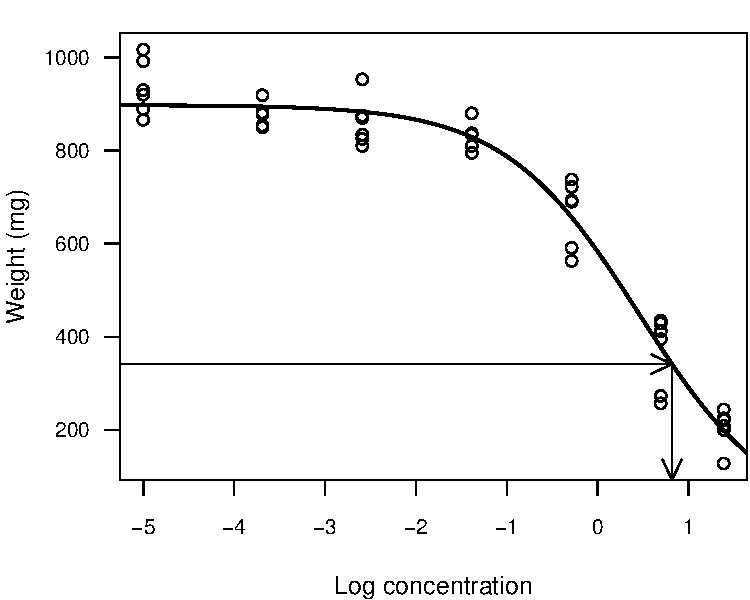
\includegraphics[width=\maxwidth]{figure/nasturtium-scatter} \caption[Scatterplot of the nasturtium data]{Scatterplot of the nasturtium data with fitted logit-log model. The horizontal arrow corresponds to the observed $\bar{y}_0 = 341.333$ mg and the vertical arrow corresponds to the logarithm of the estimated concentration $\log(\wh{x}_0) = 0.817$.\label{fig:nasturtium-scatter}}
\end{figure}


\end{knitrout}


A logit-log regression function is used to describe the data:
\begin{equation*}
  \mu(x; \beta_1, \beta_2, \beta_3) = \left\{ \begin{array}{l l}
                                              \beta_1, &\quad x = 0 \\
                                              \beta_1 / \left[1 + \exp\left\{\beta_2 + \beta_3\ln(x)\right\}\right], &\quad x > 0,
                                            \end{array} \right..
\end{equation*}
The errors are assumed to be normally distributed with mean zero and constant variance $\sigma_\epsilon^2$. Normality was checked using a normal Q-Q plot of the residuals and the constant variance assumption appears reasonable from the scatterplot. In the second stage of the experiment, the observed weights corresponding to three new soil samples all sharing the same concentration $x_0$ were observed to be 309, 296, and 419 mg. An estimate of the unknown concentration is obtained by inverting the fitted calibration curve and found to be 2.2639. We follow Poon in assuming, \textit{a priori}, that $x_0$ is independent of $(\beta_1, \beta_2, \beta_3, \sigma_\epsilon^2)$. Improper uniform priors were given to the parameters $(\beta_1, \beta_2, \beta_3, \sigma_\epsilon^2)$, and the prior for $x_0$ was chosen to be uniform over the experimental range: $x_0 \sim \mc{U}(0, 4)$. The posterior for $x_0$ is shown in Figure~\ref{fig:nasturtium-post-boot} and is nearly identical to the approximation obtained by \citet[fig. 9]{racine-poon_bayesian_1988}. A histogram of the bootstrap distribution of $\wh{x}_0$ is also shown in Figure~\ref{fig:nasturtium-post-boot} for comparison. The mean of the posterior density is 2.3434, and the mode is 2.3124. A corresponding 95\% HPD interval for the unknown $x_0$ is (1.7566, 3.0011). For comparison, we also provide the inversion, Wald, and $BC_a$ intervals for $x_0$ in Table~\ref{tab:results}. If our prior information accurately reflects the truth, then the HPD interval is preferred. Otherwise, the inversion or bootstrap interval are both reasonable. The bootstrap distribution and posterior density in Figure~\ref{fig:nasturtium-post-boot} are clearly skewed to the right; thus, a symmetric interval, such as the Wald interval, may not be appropriate here.

\begin{knitrout}
\definecolor{shadecolor}{rgb}{0.969, 0.969, 0.969}\color{fgcolor}\begin{figure}[!htb]

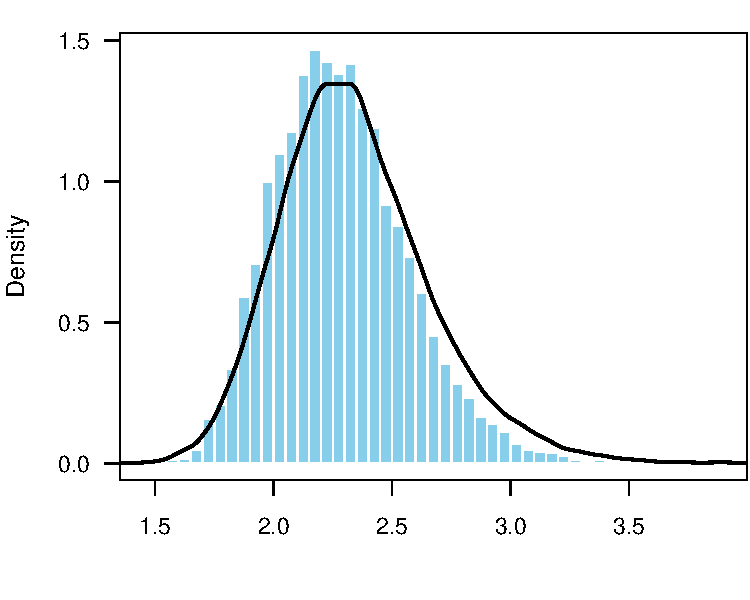
\includegraphics[width=\maxwidth]{figure/nasturtium-post-boot} \caption[Posterior and bootstrap results for the nasturtium example]{Posterior of $x_0$ (solid curve) together with the bootstrap distribution of $\wh{x}_0$ (histogram).\label{fig:nasturtium-post-boot}}
\end{figure}


\end{knitrout}


%% Table of results
\begin{table}
\centering
\caption[ 95\% calibration intervals for the nasturtium data]{Comparison of 95\% calibration intervals for the nasturtium example. \label{tab:results}}
\begin{tabular}{lcc}
  \toprule
  Inversion interval & (1.772, 2.969) \\ 
  Wald interval      & (1.689, 2.839) \\ 
  $BC_a$ interval    & (1.805, 2.903) \\ 
  HPD interval       & (1.7566, 3.0011) \\ 
  \bottomrule
\end{tabular}
\end{table}



%% Nonparametric Calibration ---------------------------------------------------

% !Rnw root = Master.Rnw

\chapter{Semiparametric Calibration}
\label{chap:nonparametric}
So far, we have considered calibration curves in which the mean response $\mu(x) = \E\left\{\mc{Y} | x\right\}$ has a known form that depends on a small number of unknown parameters $\bm{\beta}$. Finding a good parametric model, however, can be time consuming and require a great deal of expertise. Therefore, it is sometimes useful to assess the effects of the explanatory variable $x$ without completely specifying the structural form of $\mu(x)$. In this chapter, we propose a simple and fast \textit{semiparametric} approach to computing calibration curves. By ``semiparametric'', we mean that only part of the model is specified. Our treatment of semiparametric calibration curves follows the work of \citet{brumback_comment_1999}, \citet{ruppert_selecting_2002}, and \citet{ruppert_semiparametric_2003}, and \citet{crainiceanu_bayesian_2005}. Nonparametric calibration has also been discussed in the literature by, for example, \citet{clark_calibration_1979}, \citet{clark_calibration_1980}, and \citet{rosen_constructing_1995}. Our approach to calibration here is similar to that of \citet{clark_calibration_1980} in that we are inverting bias-adjusted prediction intervals. However, the \ac{LMM} representation of \ac{P-spline}s \citep{ruppert_semiparametric_2003} we use here yields a rather simple method for making this adjustment. Rosen and Cohen used a nonparametric bootstrap to obtain calibration intervals from a cubic smoothing spline. Their approach, however, made no attempt to correct for bias in the smoothed calibration curve.

In Section~\ref{sec:pspline-lmm}, we discuss the linear mixed-effects model representation of \ac{P-spline}s. Section~\ref{sec:adjusted-calibration} proposes a method for obtaining bias-adjusted calibration intervals based on the mixed model representation. A small Monte Carlo study demonstrates that the these intervals have coverage probability close to the nominal $1-\alpha$ level. A Bayesian analog of this procedure is proposed in Section~\ref{sec:pspline-bayesian}. Section~\ref{sec:semipar-discussion} concludes this chapter with a discussion on ideas for future research.

\section{Mixed model representation of P-splines}
\label{sec:pspline-lmm}
Recall the polynomial spline model from Section~\ref{sec:penalized-regression-splines}:
\begin{equation}
  \mc{Y}_i = \sum_{j = 0}^p\beta_jx_i^j + \sum_{k = 1}^K \alpha_k\left(x_i - \xi_k\right)_+^p + \epsilon_i, \quad \epsilon_i \stackrel{iid}{\sim} \left(0, \sigma_\epsilon^2\right), \quad i = 1, \dotsc, n.
\end{equation}
We can easily write this in matrix form, such as in Equation~\eqref{eqn:spline-model-matrix}, but a more useful form is obtained by separating the polynomial and spline terms as in
\begin{equation}
\label{eqn:spline-model-lme}
  \bc{Y} = \bm{X}\bm{\beta} + \bm{Z}\bm{\alpha} + \bm{\epsilon}, \quad \bm{\epsilon} \sim \left(\bm{0}, \sigma_\epsilon^2\bm{I}\right),
\end{equation}
where $\bm{\beta} = (\beta_0, \beta_1, \dotsc, \beta_p)'$ are the coefficients of the polynomial basis functions, $\bm{\alpha} = (\alpha_1, \dotsc, \alpha_K)'$ are the coefficients of the spline basis functions, and $\bm{X}$ and $\bm{Z}$ are known design matrices with $i$-th rows equal to
\begin{equation*}
\bm{X}_i = \left(1, x_i, x_i^2, \dotsc, x_i^p \right)' \quad \text{and} \quad  \bm{Z}_i = \left( (x_i - \xi_1)_+^p, \dotsc, (x_i - \xi_K)_+^p \right)',
\end{equation*}
respectively. Although we choose $\bm{Z}$ to be the truncated polynomial spline basis matrix, any other basis will do (e.g., radial basis, B-spline basis, etc.). Based on the matrix Equation~\eqref{eqn:spline-model-lme}, the penalized spline fitting criterion, Equation~\eqref{eqn:pss}, becomes
\begin{equation*}
  \norm{\bc{Y} - \bm{X}\bm{\beta} - \bm{Z}\bm{\alpha}}^2 + \lambda^{2p}\norm{\bm{\alpha}}^2,
\end{equation*}
which is proportional to Equation~\eqref{eqn:lmm-pss}, the PSS for an \ac{LMM} with hierarchical structure $\bc{Y}|\bm{\alpha} \sim \mc{N}(\bm{X}\bm{\beta} + \bm{Z}\bm{\alpha}, \sigma_\epsilon^2\bm{I})$ and $\bm{\alpha} \sim \mc{N}(0, \sigma_\alpha^2\bm{I})$. Dividing through by the error variance, $\sigma_\epsilon^2$, gives the smoothing parameter as $\lambda^{2p} = \sigma_\epsilon^2/\sigma_\alpha^2$, a simple ratio of the variance components. This leads to the following mixed model representation of \ac{P-spline}s \citep{brumback_comment_1999}:
\begin{equation}
\label{eqn:pspline-lmm}
  \bc{Y} = \bm{X}\bm{\beta} + \bm{Z}\bm{\alpha} + \bm{\epsilon}, \quad 
  \begin{bmatrix} 
    \bm{\alpha} \\
    \bm{\epsilon}
  \end{bmatrix} \sim 
    \mc{N}\left(\begin{bmatrix} 
      \bm{0} \\
      \bm{0}
    \end{bmatrix}, \begin{bmatrix} 
    \sigma_\alpha^2\bm{I} & \bm{0} \\
    \bm{0} & \sigma_\epsilon^2\bm{I}
  \end{bmatrix}\right).
\end{equation}
The parameters $\bm{\beta}$, $\bm{\alpha}$, $\sigma_\alpha^2$, and $\sigma_\epsilon^2$ can all be estimated using standard mixed model methodology and software. Under this framework, a \ac{P-spline} is really just the \ac{BLUP} from a special \ac{LMM}! The amount of smoothing is determined automatically by $\wh{\lambda} = \wh{\sigma}_\epsilon^2/\wh{\sigma}_\alpha^2$, where $\wh{\sigma}_\epsilon^2$ and $\wh{\sigma}_\alpha^2$ are the \ac{REML} estimates of $\sigma_\epsilon^2$ and $\sigma_\alpha^2$, respectively. Although $\lambda$ could be estimated via ordinary \ac{ML} estimation or cross-validation, \citet{krivobokova_note_2007} showed that the \ac{REML}-based estimate is less affected by the presence of different correlation structures for the errors, $\bm{\epsilon}$. The \ac{BLUP} of $\bm{\mu}$, denoted $\wt{\bm{\mu}}$, was given in Equation~\eqref{eqn:mu-blup}; however, an equivalent expression for $\wt{\bm{\mu}}$ is given by
\begin{equation*}
  \wt{\bm{\mu}} = \bm{\Omega}\left( \bm{\Omega}'\bm{\Omega} + \frac{\sigma_\epsilon^2}{\sigma_\alpha^2}\bm{D} \right)^{-1}\bm{\Omega}'\bc{Y} = \bm{S}\bc{Y}, \quad \bm{\Omega} = \left(\bm{X}; \bm{Z}\right),
\end{equation*}
where $\textbf{D} = \diag\left\{\bm{0}_{(p+1) \times (p+1)}, \bm{I}_{K \times K}\right\}$. The vector of fitted values (i.e., the \ac{EBLUP} of $\bm{\mu}$) is then just
\begin{equation*}
  \wh{\bm{\mu}} = \bm{\Omega}\left( \bm{\Omega}'\bm{\Omega} + \frac{\wh{\sigma}_\epsilon^2}{\wh{\sigma}_\alpha^2}\bm{D} \right)^{-1}\bm{\Omega}'\bc{Y},
\end{equation*}
where $\wh{\sigma}_\epsilon^2$ and $\wh{\sigma}_\alpha^2$ are the \ac{REML} estimates of $\sigma_\epsilon^2$ and $\sigma_\alpha^2$, respectively.

As described in \citet{robinson_that_1991}, the \ac{LMM} has a simple Bayesian analog. For the mixed model representation, Equation~\eqref{eqn:pspline-lmm}, if $\bm{\beta}$, $\sigma_\epsilon^2$, and $\sigma_\alpha^2$ are all given improper uniform priors, then the posterior of $\bm{\mu}$ is $\mc{N}\left( \wh{\bm{\mu}}, \sigma_\epsilon^2 \bm{S} \right)$. Note the use of the variance-covariance matrix $\sigma_\epsilon^2\bm{S}$ rather than the variance-covariance matrix $\sigma_\epsilon^2\bm{S}\bm{S}'$ from Equation~\eqref{eqn:cov}. It is easy to see that $\left[\bm{S}\right]_{ij} \ge \left[\bm{S}\bm{S}'\right]_{ij}$; hence, confidence and prediction intervals based on the Bayesian variance-covariance matrix $\sigma_\epsilon^2\bm{S}$ are wider than those based on $\sigma_\epsilon^2\bm{S}\bm{S}'$. As pointed out by \citet{hastie_gams_1990}, the ``extra wideness'' is due to the fact that $\bm{S}$ accounts for squared bias whereas $\bm{S}\bm{S}'$ does not.

\section{Bias-adjusted calibration intervals}
\label{sec:adjusted-calibration}
As mentioned in Section~\ref{sec:pspline-inference}, the estimated mean response $\wh{\mu}(x)$ is biased. Inference for \ac{P-spline}s based on the \ac{LMM} representation, Equation~\eqref{eqn:pspline-lmm}, differs depending on whether we take the randomness of $\bm{\alpha}$ into account. Ignoring the randomness in $\bm{\alpha}$ leads to the same intervals given in Section~\ref{sec:pspline-inference}. We can account for bias in the confidence and prediction intervals, however, by conditioning on the random effects $\bm{\alpha}$. To see this, note that the bias vector of $\wt{\bm{\mu}}$, conditional on $\bm{\alpha}$, is 
\begin{equation}
\label{eqn:conditional-bias}
  \E\left\{\wt{\bm{\mu}} - \bm{\mu} | \bm{\alpha}\right\} = \bm{X}\left[ \E\left\{\wt{\bm{\beta}} | \bm{\alpha}\right\} - \bm{\beta} \right] + \bm{Z}\Big[ \E\left\{\wt{\bm{\alpha}} | \bm{\alpha}\right\} - \bm{\alpha} \Big].
\end{equation}

From the properties of conditional expectation \citep[pg. 164]{casella_statistical_2002}, we have that $\E\left\{\E\left(\wt{\bm{\beta}}|\bm{\alpha}\right)\right\} = \E\left\{\wt{\bm{\beta}}\right\}$ and $\E\left\{\E\left(\wt{\bm{\alpha}}|\bm{\alpha}\right)\right\} = \E\left\{\wt{\bm{\alpha}}\right\}$. But since $\E\left\{\wt{\bm{\beta}}\right\} = \bm{\beta}$ and $\E\left\{\wt{\bm{\alpha}}\right\} = \E\left\{\bm{\alpha}\right\} = \bm{0}$, the unconditional bias is just 
\begin{equation*}
  %\E\left(\wt{\bm{\mu}} - \bm{\mu}\right) = 
  \E\left\{\E\left(\wt{\bm{\mu}} - \bm{\mu}|\bm{\alpha}\right)\right\} = \bm{X}\left(\bm{\beta} - \bm{\beta}\right) + \bm{Z}\left(\bm{0} - \bm{0}\right) = \bm{0}. 
\end{equation*}
Thus, $\wt{\bm{\mu}}$ is unbiased for $\bm{\mu}$ when averaged over the distribution of $\bm{\alpha}$. This is equivalent to the Bayesian approach where (pointwise) confidence and prediction bands use diagonal entries of $\bm{S}$ in place of the diagonal entries of $\bm{S}\bm{S}'$ described in Section~\ref{sec:pspline-inference}.

Let $\bm{\Omega}_0 = \left(1, x_0, \dotsc, x_0^p, (x_0 - \xi_1)_+^p, \dotsc, (x_0 - \xi_K)_+^p\right)'$ where $x_0$ is an arbitrary value of the explanatory variable $x$. A $100(1 - \alpha)\%$ (bias-adjusted) confidence interval for $\mu(x_0)$ is given by
\begin{equation*}
  \wh{\mu}(x_0) \pm \tquant{1-\alpha/2}{df} \times \wh{\sigma}_\epsilon\sqrt{\bm{\Omega}_0\left(\bm{\Omega}\bm{\Omega}' + \frac{\wh{\sigma}_\epsilon^2}{\wh{\sigma}_\alpha^2}\bm{D} \right)^{-1}\bm{\Omega}_0'},
\end{equation*}
where $df = n - 2\tr\left(\bm{S}\right) + \tr\left(\bm{S}\bm{S}'\right)$. In a similar manner, a $100(1 - \alpha)\%$ (bias-adjusted) prediction interval for a new observation, $\mc{Y} = \mu(x_0) + \epsilon_0$ (independent of current ones), is given as
\begin{equation}
\label{eqn:bias-adjusted-pi}
  \wh{\mu}(x_0) \pm \tquant{1-\alpha/2}{df} \times \wh{\sigma}_\epsilon\sqrt{1 + \bm{\Omega}_0\left(\bm{\Omega}\bm{\Omega}' + \frac{\wh{\sigma}_\epsilon^2}{\wh{\sigma}_\alpha^2}\bm{D} \right)^{-1}\bm{\Omega}_0'}.
\end{equation}

Recall the intuition behind the inversion interval. Let $I_\mathrm{pred}(x)$ be a $100(1 - \alpha)\%$ prediction interval for the future observation $\mc{Y}_0$, such that $\Pr\left\{ \mc{Y}_0 \in I_\mathrm{pred}(x) | x_0 = x \right\} = 1 - \alpha$. Then, a confidence interval for $x_0$ corresponding to an observed $\mc{Y}_0$ is just the set $\mc{J}_\mathrm{cal}(x) = \left\{x : \mc{Y}_0 \in I_\mathrm{pred}(x)\right\}$ since, by construction, 
\begin{equation*}
\Pr\left\{x_0 \in \mc{J}_\mathrm{cal}(\mc{Y}_0)\right\} = \Pr\left\{\mc{Y}_0 \in I_\mathrm{pred}(x) | x_0 = x\right\} = 1 - \alpha,
\end{equation*}
\citep{clark_calibration_1980}. In other words, a $100(1 - \alpha)\%$ confidence interval for $x_0$ can be obtained by inverting a corresponding prediction interval for $\mc{Y}_0$. However, we need to invert an appropriate prediction interval (i.e., one that adjusts for bias); otherwise, the resulting confidence interval for $x_0$ will likely not be reliable. To that end, we propose the following bias-adjusted $100(1-\alpha)\%$ calibration interval for the unknown $x_0$:
% \begin{equation}
% \label{eqn:bc-inversion-interval}
%   \wh{\mc{J}}_\mathrm{cal}^{\mathrm{ba}}(x_0) = \left\{x_0: \frac{\left[y_0 - \wh{\mu}(x_0)\right]^2}{\wh{\sigma}_\epsilon^2\left[1 + \bm{\Omega}_0\left(\bm{\Omega}'\bm{\Omega} + \frac{\wh{\sigma}_\epsilon^2}{\wh{\sigma}_\alpha^2}\bm{D}\right)^{-1}\bm{\Omega}_0'\right]} < \mc{F}_{1, df}^{1-\alpha}\right\},
% \end{equation}
\begin{equation}
\label{eqn:bc-inversion-interval}
  \wh{\mc{J}}_\mathrm{cal}^{\mathrm{ba}}(x_0) = \left\{x_0: \tquant{\alpha/2}{df} < \frac{y_0 - \wh{\mu}(x_0)}{\sqrt{\wh{\sigma}_\epsilon^2\left[1 + \bm{\Omega}_0\left(\bm{\Omega}'\bm{\Omega} + \frac{\wh{\sigma}_\epsilon^2}{\wh{\sigma}_\alpha^2}\bm{D}\right)^{-1}\bm{\Omega}_0'\right]}} < \tquant{1-\alpha/2}{df}\right\},
\end{equation}
As before, great care should be taken to ensure that $\wh{\mc{J}}_\mathrm{cal}^{\mathrm{ba}}(x_0)$ is an interval. This may not be the case, for example, when $\mu(x)$ in not monotonic over the range of interest. Also, as with nonlinear calibration, no closed-form expression exists for $\wh{\mc{J}}_\mathrm{cal}^{\mathrm{ba}}(x)$ and iterative techniques are required. In a similar fashion, a $100(1-\alpha)\%$ bias-adjusted regulation interval for $x_0$ is obtained by inverting a corresponding bias-adjusted confidence interval for the mean response:
\begin{equation*}
  \wh{\mc{J}}_\mathrm{reg}^{\mathrm{ba}}(x_0) = \left\{x_0: \tquant{\alpha/2}{df} < \frac{y_0 - \wh{\mu}(x_0)}{\sqrt{\wh{\sigma}_\epsilon^2\bm{\Omega}_0\left(\bm{\Omega}'\bm{\Omega} + \frac{\wh{\sigma}_\epsilon^2}{\wh{\sigma}_\alpha^2}\bm{D}\right)^{-1}\bm{\Omega}_0'}} < \tquant{1-\alpha/2}{df}\right\}.
\end{equation*}

We designed a small Monte Carlo study to investigate the coverage probability of this technique. The results of this study are presented in Tables~\ref{tab:pspline-monte-carlo-1} and \ref{tab:pspline-monte-carlo-2}. The true calibration function is the sine wave $\mu(x) = \sin(\pi x - \pi/2)/2 + 1/2$ plotted in Figure~\ref{fig:sine-wave}. For data following such a pattern, it would be tempting to fit a nonlinear model, perhaps modeling $\mu(x)$ as a \textit{logistic} function. Inference based on the resulting fit would then be inaccurate since, for example, the true calibration curve does not have any asymptotes. For situations like this, it would be useful to have a semiparametric alternative for which to compare inference.

\begin{knitrout}
\definecolor{shadecolor}{rgb}{0.969, 0.969, 0.969}\color{fgcolor}\begin{figure}[H]

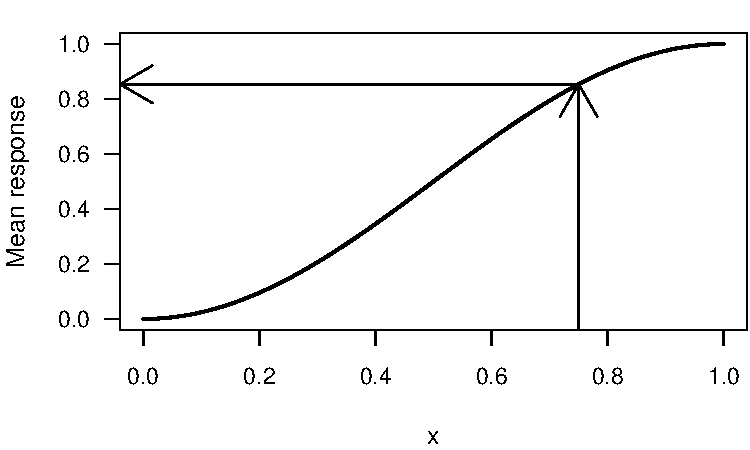
\includegraphics[width=\maxwidth]{figure/sine-wave} \caption[Scaled sine wave function]{Scaled sine wave function.\label{fig:sine-wave}}
\end{figure}


\end{knitrout}


Notice that the sine wave plotted in Figure~\ref{fig:sine-wave} is scaled to lie in $[0, 1] \times [0, 1]$ with a period of 2. For each of 1,000 simulations, we used $10$, $30$, and $50$ uniformly spaced designed points on the domain $[0, 1]$ with $1$, $2$, and $3$ independent replicates of the response at each design point. The errors were generated as i.i.d. $\mc{N}(0, 0.05^2)$ random variates and the true unknown was chosen to be $x_0 = 0.75$ (hence, $\mu_0 \approx 0.8536$).

Tables~\ref{tab:pspline-monte-carlo-1} and \ref{tab:pspline-monte-carlo-2} display the estimated coverage probability for this technique applied to the sine wave experiment for both calibration (Table~\ref{tab:pspline-monte-carlo-1}) and regulation (Table~\ref{tab:pspline-monte-carlo-2}). For comparison, we also transformed the data to an equivalent linear model and applied Fieller's method (which yields an exact $95\%$ confidence interval for $x_0$). Clearly, our bias-adjusted intervals performed well for quadratic (degree = 2) and cubic (degree = 3) \ac{P-spline}s with increasing sample size without sacrificing interval length. Notice, however, that the calibration results are somewhat conservative (i.e., the coverage probability is slightly larger than $0.95$) while the regulation intervals tend to hit the target coverage $1-\alpha = 0.95$. The reason for this is that the bias in predicting a future observation is the same as that for estimating the mean response, but the former has larger variance. Therefore, the bias accounts for a smaller portion of the mean-squared error in prediction (i.e., the bias gets ``washed out'' by a larger variance). Thus, for larger samples (perhaps $n \ge 20$ with $m \ge 1$ replicates at each design point), calibration intervals could be computed with or without adjusting for bias. Regulation intervals, on the other hand, should always be adjusted for bias.




% \begin{table}[H]%[!htb]
% \centering
%   \begin{tabular}{llcccccccc}
%   \toprule
%   \phantom{abc} & \phantom{abc} & \multicolumn{2}{c}{P-spline $\left(p=1\right)$} & \multicolumn{2}{c}{P-spline $\left(p=2\right)$} & \multicolumn{2}{c}{P-spline $\left(p=3\right)$} & \multicolumn{2}{c}{Fieller} \\
%   \cline{3-10}
%   $n$ & $m$ & CP & Length & CP & Length & CP & Length & CP & Length \\
%   \hline
%   10  &  1  & sim1[1,1] & sim1[1,2] & sim1[10,1] & sim1[10,2] & sim1[19,1] & sim1[19, 2] & sim2[1, 1] & sim2[1, 2] \\
%   10  &  2  & sim1[2,1] & sim1[2,2] & sim1[11,1] & sim1[11,2] & sim1[20,1] & sim1[20, 2] & sim2[2, 1] & sim2[2, 2] \\
%   10  &  3  & sim1[3,1] & sim1[3,2] & sim1[12,1] & sim1[12,2] & sim1[21,1] & sim1[21, 2] & sim2[3, 1] & sim2[3, 2] \\
%   \hline
%   30  &  1  & sim1[4,1] & sim1[4,2] & sim1[13,1] & sim1[13,2] & sim1[22,1] & sim1[22, 2] & sim2[4, 1] & sim2[4, 2] \\
%   30  &  2  & sim1[5,1] & sim1[5,2] & sim1[14,1] & sim1[14,2] & sim1[23,1] & sim1[23, 2] & sim2[5, 1] & sim2[5, 2] \\
%   30  &  3  & sim1[6,1] & sim1[6,2] & sim1[15,1] & sim1[15,2] & sim1[24,1] & sim1[24, 2] & sim2[6, 1] & sim2[6, 2] \\
%   \hline
%   50  &  1  & sim1[7,1] & sim1[7,2] & sim1[16,1] & sim1[16,2] & sim1[25,1] & sim1[25, 2] & sim2[7, 1] & sim2[7, 2] \\
%   50  &  2  & sim1[8,1] & sim1[8,2] & sim1[17,1] & sim1[17,2] & sim1[26,1] & sim1[26, 2] & sim2[8, 1] & sim2[8, 2] \\
%   50  &  3  & sim1[9,1] & sim1[9,2] & sim1[18,1] & sim1[18,2] & sim1[27,1] & sim1[27, 2] & sim2[9, 1] & sim2[9, 2] \\
%   \bottomrule
%   \end{tabular}
% \caption[Semiparametric calibration Monte Carlo simulation]{Coverage and length of $95\%$ calibration intervals for data from the sine wave experiment with $\sigma_\epsilon = 0.05$. \label{tab:pspline-monte-carlo-1}}
% \end{table}

\begin{table}[H]%[!htb]
\centering
\caption[Semiparametric calibration Monte Carlo simulation]{Coverage and length of $95\%$ calibration intervals for data from the sine wave experiment with $\sigma_\epsilon = 0.05$. \label{tab:pspline-monte-carlo-1}}
  \begin{tabular}{llcccccccc}
  \toprule
  \phantom{abc} & \phantom{abc} & \multicolumn{2}{c}{P-spline $\left(p=1\right)$} & \multicolumn{2}{c}{P-spline $\left(p=2\right)$} & \multicolumn{2}{c}{P-spline $\left(p=3\right)$} & \multicolumn{2}{c}{Fieller} \\
  \cline{3-10}
  $n$ & $m$ & CP & Length & CP & Length & CP & Length & CP & Length \\
  \hline
  10  &  1  & 0.93 & 0.25 & 0.93 & 0.21 & 0.90 & 0.19 & 0.95 & 0.25 \\
  10  &  2  & 0.96 & 0.21 & 0.97 & 0.20 & 0.96 & 0.19 & 0.96 & 0.22 \\
  10  &  3  & 0.97 & 0.21 & 0.96 & 0.20 & 0.97 & 0.19 & 0.96 & 0.21 \\
  \hline
  30  &  1  & 0.95 & 0.21 & 0.95 & 0.20 & 0.97 & 0.18 & 0.96 & 0.21 \\
  30  &  2  & 0.96 & 0.20 & 0.96 & 0.19 & 0.97 & 0.18 & 0.95 & 0.20 \\
  30  &  3  & 0.97 & 0.20 & 0.96 & 0.19 & 0.97 & 0.18 & 0.96 & 0.20 \\
  \hline
  50  &  1  & 0.97 & 0.20 & 0.96 & 0.19 & 0.96 & 0.18 & 0.96 & 0.20 \\
  50  &  2  & 0.97 & 0.20 & 0.97 & 0.19 & 0.96 & 0.18 & 0.95 & 0.20 \\
  50  &  3  & 0.98 & 0.20 & 0.97 & 0.19 & 0.97 & 0.18 & 0.96 & 0.20 \\
  \bottomrule
  \end{tabular}
\end{table}

\begin{table}[H]%[!htb]
\centering
\caption[Semiparametric regulation Monte Carlo simulation]{Coverage and length of $95\%$ regulation intervals for data from the sine wave experiment with $\sigma_\epsilon = 0.05$. \label{tab:pspline-monte-carlo-2}}
  \begin{tabular}{llcccccccc}
  \toprule
  \phantom{abc} & \phantom{abc} & \multicolumn{2}{c}{Degree = 1} & \multicolumn{2}{c}{Degree = 2} & \multicolumn{2}{c}{Degree = 3} & \multicolumn{2}{c}{Fieller} \\
  \cline{3-10}
  $n$ & $m$ & CP & Length & CP & Length & CP & Length & CP & Length \\
  \hline
  10  &  1  & 0.74 & 0.13 & 0.92 & 0.12 & 0.92 & 0.11 & 0.95 & 0.10 \\
  10  &  2  & 0.89 & 0.09 & 0.94 & 0.09 & 0.94 & 0.08 & 0.95 & 0.06 \\
  10  &  3  & 0.91 & 0.07 & 0.95 & 0.07 & 0.94 & 0.06 & 0.95 & 0.05 \\
  \hline
  30  &  1  & 0.96 & 0.07 & 0.95 & 0.07 & 0.94 & 0.06 & 0.95 & 0.05 \\
  30  &  2  & 0.97 & 0.06 & 0.95 & 0.05 & 0.94 & 0.04 & 0.95 & 0.04 \\
  30  &  3  & 0.97 & 0.05 & 0.95 & 0.04 & 0.95 & 0.03 & 0.95 & 0.03 \\
  \hline
  50  &  1  & 0.96 & 0.06 & 0.95 & 0.05 & 0.95 & 0.05 & 0.95 & 0.04 \\
  50  &  2  & 0.97 & 0.04 & 0.96 & 0.04 & 0.95 & 0.03 & 0.95 & 0.03 \\
  50  &  3  & 0.97 & 0.04 & 0.96 & 0.03 & 0.95 & 0.03 & 0.95 & 0.02 \\
  \bottomrule
  \end{tabular}
\end{table}

\subsection{Whiskey age example}
\label{sec:whiskey}
The point of this example is to demonstrate how our bias-adjusted semiparametric approach to calibration compares against a simpler parametric model (when one is available). To this end, we analyze the whiskey data from \citet{schoeneman_analytical_1971} presented in Figure~\ref{fig:whiskey-scatter}. The data give the proof (measured as twice the percentage of alcohol by volume, denoted 2ABV) of whiskey stored in a charred oak barrel against time in years; clearly, some curvature is present. Suppose a new sample is obtained from the same barrel and that the proof is observed to be $y_0 = 108 \text{ 2ABV}$. It is desired to estimate how long this batch has been aged.

\begin{knitrout}
\definecolor{shadecolor}{rgb}{0.969, 0.969, 0.969}\color{fgcolor}\begin{kframe}


{\ttfamily\noindent\itshape\color{messagecolor}{\#\# Loading required package: rootSolve}}\end{kframe}\begin{figure}[H]

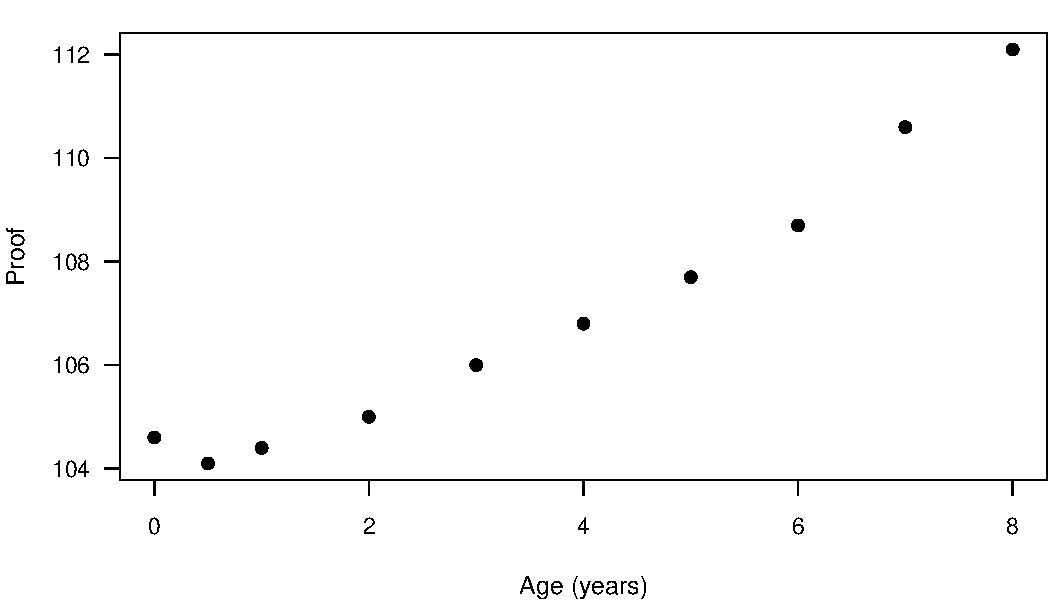
\includegraphics[width=\maxwidth]{figure/whiskey-scatter} \caption[Scatterplot of the whiskey data]{Scatterplot of the whiskey data.\label{fig:whiskey-scatter}}
\end{figure}


\end{knitrout}


We begin by fitting a simple quadratic \ac{P-spline} with five knots:
\begin{equation*}
  \mu(\text{\texttt{age}}_i) = \beta_0 + \beta_1\text{\texttt{age}}_i + \beta_2\text{\texttt{proof}}_i^2 + \sum_{k = 1}^5\alpha_k\left( \text{\texttt{proof}}_i - \xi_k \right)_+^2.
\end{equation*}
The number of knots and their placement were determined automatically using the methods described in Section~\ref{sec:penalized-regression-splines}. The fitted model is depicted in the right-hand side of Figure~\ref{fig:whiskey-calibration}. It appears from the scatterplot that a simple quadratic may be sufficient (i.e., $\alpha_i = 0$, $i = 1, \dotsc, 5$); this fit is depicted in the left side of Figure~\ref{fig:whiskey-calibration}. Both models are different, but the fits are indistinguishable to the human eye. In fact, both models produce identical calibration intervals for $x_0$ (when rounded to four decimal places). For the linear model, we have $\wh{x}_0 = 5.2329$ years with a 95\% confidence interval for $x_0$ of $(4.6776, 5.7352)$. Similarly, for the \ac{P-spline} model, we have $\wh{x}_0 = 5.2329$ years with a 95\% (bias-adjusted) confidence interval for $x_0$ of $(4.6776, 5.7352)$. The reason we get the same answer from both models is that the polynomial basis part of the penalized spline model is sufficient for modeling the curvature of $\mu(\texttt{age})$, therefore, the spline basis terms are effectively ``zeroed out'' (see Figure~\ref{fig:whiskey-paths}). Although our \ac{P-spline} approach to obtaining calibration intervals requires large samples, in this small sample example, they happen to coincide with the classical inversion limits from the quadratic linear model. If we did not correct for bias in the \ac{P-spline} model, however, the confidence interval obtained for $x_0$ would be $(4.7223, 5.7016)$, which is too narrow.

\begin{knitrout}
\definecolor{shadecolor}{rgb}{0.969, 0.969, 0.969}\color{fgcolor}\begin{figure}[H]

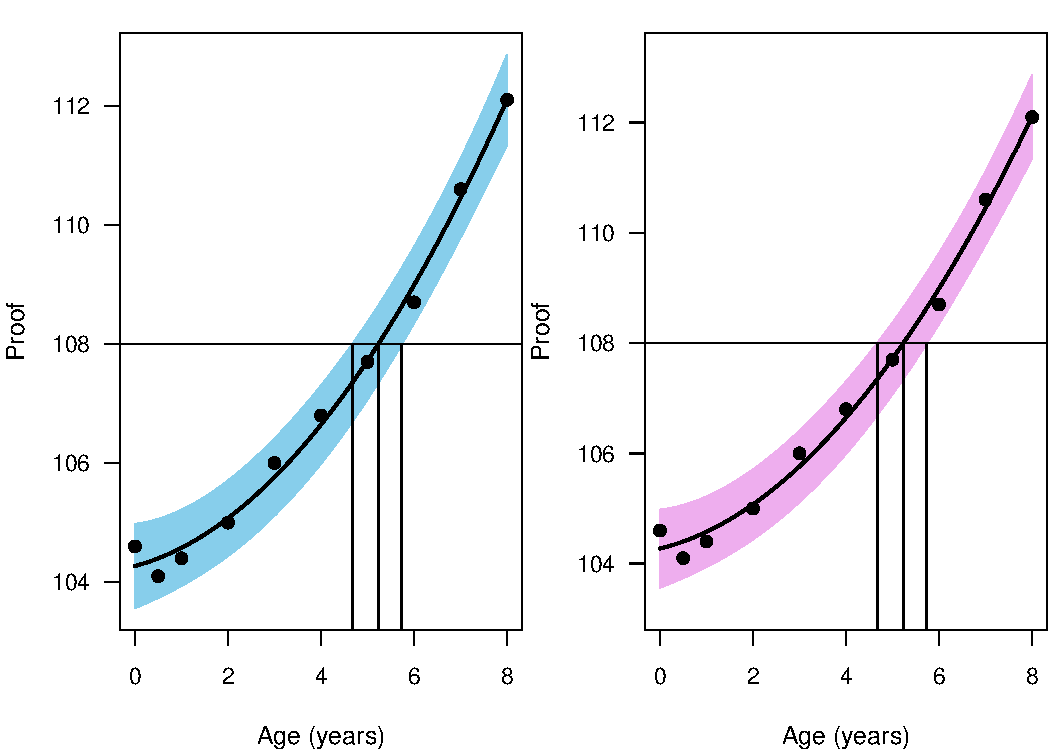
\includegraphics[width=\maxwidth]{figure/whiskey-calibration} \caption[Fitted  models for the whiskey data]{Fitted  models for the whiskey data. \textit{Left}: Quadratic linear model with 95\% (pointwise) prediction band. \textit{Right}: Quadratic \ac{P-spline} with five knots and 95\% (pointwise) bias-adjusted prediction band.\label{fig:whiskey-calibration}}
\end{figure}


\end{knitrout}


\begin{knitrout}
\definecolor{shadecolor}{rgb}{0.969, 0.969, 0.969}\color{fgcolor}\begin{figure}[H]

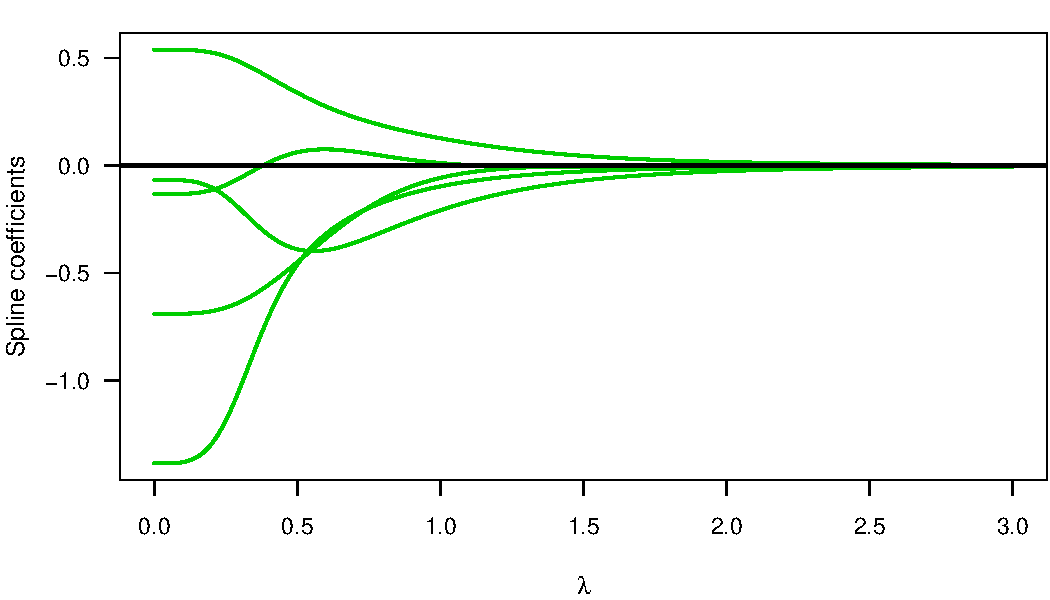
\includegraphics[width=\maxwidth]{figure/whiskey-paths} \caption[Spline coefficient paths for the whiskey example]{Profiles of spline coefficients for the \ac{P-spline} in Figure~\ref{fig:whiskey-calibration}, as the smoothing parameter $\lambda$ is varied from zero to three. Coefficients are plotted versus the smoothing parameter $\lambda$; the \ac{REML} estimate is $\wh{\lambda} = 385.2228$.\label{fig:whiskey-paths}}
\end{figure}


\end{knitrout}


\section{Bayesian semiparametric calibration}
\label{sec:pspline-bayesian}
The mixed model \ac{P-spline}, Equation~\eqref{eqn:pspline-lmm}, provides a simple method for estimating the smoothing parameter and accounting for bias in calibration intervals. These intervals, however, do not account for the variability of the estimated smoothing parameter $\wh{\lambda} = \wh{\sigma}_\epsilon^2/\wh{\sigma}_\alpha^2$ (similar to inference in \ac{LMM}s which typically ignores the variability of $\wh{\bm{V}}$). This problem can be remedied by adopting a fully Bayesian approach which we now discuss. 

Let $\pi(\cdot)$ denote a probability density function. Following \citet{hoadley_bayesian_1970}, we assume that the calibration experiment contains no information about $x_0$ and that the priors for $x_0$ and the calibration experiment are independent; thus,
\begin{equation*}
  \pi(x_0, \bm{\beta}, \bm{\alpha}, \sigma_\epsilon^2, \sigma_\alpha^2) = \pi(x_0)\pi(\bm{\beta}, \bm{\alpha}, \sigma_\epsilon^2, \sigma_\alpha^2).
\end{equation*}

The mixed model representation, Equation~\eqref{eqn:pspline-lmm}, has $\bm{\alpha} \sim \mc{N}(0, \sigma_\alpha^2\bm{I})$. A fully Bayesian approach, however, requires a prior distribution on the parameters $(\bm{\beta}, \sigma_\epsilon^2, \sigma_\alpha^2, x_0)$. Following standard convention, we assume, a priori, that the fixed-effects are independent and assign vague, independent priors to $(\bm{\beta}, \sigma_\epsilon^2, \sigma_\alpha^2)$. We used the vague (but proper) priors
\begin{align*}
  \beta_j &\sim \mc{N}\left(0, \sigma_\beta^2\right), \quad j = 1, \dotsc, p+1, \\
  \sigma_\epsilon^2 &\sim \mc{IG}\left(a, b\right), \\
  \sigma_\alpha^2 &\sim \mc{IG}\left(c, d\right),
\end{align*}
where $\mc{IG}$ stands for the inverse gamma distribution. The variance $\sigma_\beta^2$ should be chosen large enough (say $10^6$) so that (for all intents and purposes) the $\beta_j$'s are uniform. Similarly, the parameters $a$, $b$, $c$, and $d$ should be small (say $10^{-6}$). These distributions can be considered as an approximate representation of vagueness in the absence of good prior information. In addition, we assume that the prior for $x_0$, the predictor value of interest, is uniform over the experimental range: $x_0 \sim U[a, b]$. 

The (unnormalized) posterior density of $(x_0, \bm{\beta}, \bm{\alpha}, \sigma_\epsilon^2, \sigma_\alpha^2)$ is given by
\begin{align*}
  \pi(x_0, \bm{\beta}, \bm{\alpha}, \sigma_\epsilon^2, \sigma_\alpha^2 | \mathbf{data}) &= \pi(x_0, \bm{\beta}, \bm{\alpha}, \sigma_\epsilon^2, \sigma_\alpha^2 | \bm{y}, \bm{y}_0) \\
  &\propto \pi(\bm{y}, \bm{y}_0 | x_0, \bm{\beta}, \bm{\alpha}, \sigma_\epsilon^2, \sigma_\alpha^2)\pi(x_0, \bm{\beta}, \bm{\alpha}, \sigma_\epsilon^2, \sigma_\alpha^2) \\
  &\propto \pi(\bm{y}_0 | x_0, \bm{\beta}, \bm{\alpha}, \sigma_\epsilon^2, \sigma_\alpha^2)\pi(\bm{y} | \bm{\beta}, \bm{\alpha}, \sigma_\epsilon^2, \sigma_\alpha^2)\pi(\bm{\beta}, \bm{\alpha}, \sigma_\epsilon^2, \sigma_\alpha^2)\pi(x_0) \\
  &\propto \pi(\bm{y}_0 | x_0, \bm{\beta}, \bm{\alpha}, \sigma_\epsilon^2)\pi(\bm{y} | \bm{\beta}, \bm{\alpha}, \sigma_\epsilon^2)\pi(\bm{\beta})\pi(\bm{\alpha}|\sigma_\alpha^2)\pi(\sigma_\epsilon^2)\pi(\sigma_\alpha^2)\pi(x_0),
  %&\propto \pi(\bm{y}_0 | x_0, \bm{\beta}, \bm{\alpha}, \sigma_\epsilon^2, \sigma_\alpha^2)\pi(\bm{\beta}, \bm{\alpha}, \sigma_\epsilon^2, \sigma_\alpha^2 | \bm{x}, \bm{y})\pi(x_0),
\end{align*}
where $\bm{y}$ and $\bm{y}_0$ represent the observed data from the first and second stages of the calibration experiment, respectively. It is relatively straightforward to show that (see Section~\ref{sec:conditional-theta} in the appendix) the conditional posterior of $(\bm{\beta}, \bm{\alpha})$ is proportional to
\begin{equation*}
  \exp\left\{ -\frac{1}{2\sigma_\epsilon^2}\left(\norm{\bm{y}_0 - \bm{X}_0\bm{\beta} - \bm{Z}_0\bm{\alpha}}^2 + \frac{\sigma_\epsilon^2}{\sigma_\alpha^2}\norm{\bm{\alpha}}^2\right) \right\},
\end{equation*}
where
\begin{equation*}
  \bm{y}_0 = \begin{bmatrix} \bm{y} \\ y_0 \end{bmatrix}, \quad
  \bm{X}_0 = \begin{bmatrix} \bm{X} \\ \bm{x}_0' \end{bmatrix}, \quad
  \bm{Z}_0 = \begin{bmatrix} \bm{Z} \\ \bm{z}_0' \end{bmatrix}
\end{equation*}
are augmented data vectors and matrices. Upon completing the square we have that
\begin{equation*}
  \bm{\beta}, \bm{\alpha}|\bm{y}_0, \bm{y}, x_0, \sigma_\epsilon^2, \sigma_\alpha^2 \sim \mc{N}\left\{ \left(\bm{\Omega}_0'\bm{\Omega}_0 + \frac{\sigma_\epsilon^2}{\sigma_\alpha^2}\bm{D}\right)^{-1}\bm{\Omega}_0'\bm{y}_0, \sigma_\epsilon^2\left(\bm{\Omega}_0'\bm{\Omega}_0 + \frac{\sigma_\epsilon^2}{\sigma_\alpha^2}\bm{D}\right)^{-1} \right\},
\end{equation*}
where $\bm{\Omega}_0 = (\bm{X}_0, \bm{Z}_0)$. In a similar fashion, the conditional posteriors of $\sigma_\epsilon^2$ and $\sigma_\alpha^2$ are the inverse gammas:
\begin{align*}
  \sigma_\epsilon^2|\bm{y}_0, \bm{y}, \bm{\beta}, \bm{\alpha}, \sigma_\alpha^2, x_0 &\sim \mc{IG}\left( a + \frac{n+1}{2}, b + \frac{1}{2}\norm{\bm{y}_0 - \bm{X}_0\bm{\beta} - \bm{Z}_0\bm{\alpha}}^2 \right), \\
    \sigma_\alpha^2|\bm{y}_0, \bm{y}, \bm{\beta}, \bm{\alpha}, \sigma_\epsilon^2, x_0 &\sim \mc{IG}\left( c + \frac{K}{2}, d + \frac{1}{2}\norm{\bm{\alpha}}^2 \right),
\end{align*}
where $K$ is the number of knots or random effects (see Section~\ref{sec:conditional-variances} in the appendix). The conditional posterior of $x_0$ is more difficult to obtain analytically, however, regardless of the prior $\pi(x_0)$. This makes it difficult (or impossible) to obtain a full Gibbs sampler here, nonetheless, we can sample from the posterior of $x_0$ using more specialized Markov Chain Monte Carlo methods such as the \textit{Metropolis-Hastings} algorithm (see, for example, \citet[chap. 7]{robert_monte_2004}). Thus, as discussed in \citep[pg. 292]{gelman_bayesian_2003}, we could update the parameters one at a time using Gibbs sampling for $\left(\bm{\beta}, \bm{\alpha}, \sigma_\epsilon^2, \sigma_\alpha^2\right)$ and a metropolis update for $x_0$. We illustrate this approach with the following example involving radioimmunoassays. The data were analyzed using the \code{JAGS} software within \code{R} via the \pkg{rjags} package.

\subsection{Enzyme-linked immunosorbent assay (ELISA) example}
\citet{ori_constructing_1995} derived a $95\%$ calibration interval for the unknown concentration in a radioimmunoassay problem using the nonparametric bootstrap. We demonstrate our method on the same dataset and compare the results. The data, plotted in Figure~\ref{fig:elisa-scatter}, consists of 23 distinct concentrations with four (independent) replicates of the response at each concentration. The results from analyzing these data are summarized in Table~\ref{tab:elisa} at the end of this section.

\begin{knitrout}
\definecolor{shadecolor}{rgb}{0.969, 0.969, 0.969}\color{fgcolor}\begin{figure}[H]

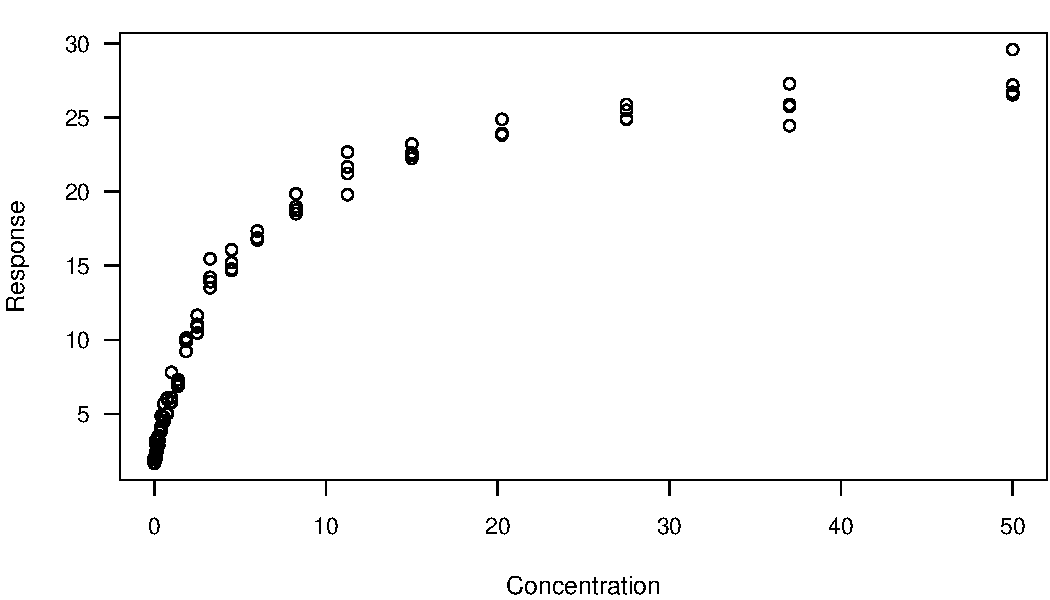
\includegraphics[width=\maxwidth]{figure/elisa-scatter} \caption[Scatterplot of the ELISA data]{Scatterplot of the ELISA data.\label{fig:elisa-scatter}}
\end{figure}


\end{knitrout}


The four parameter logistic model, 
\begin{equation*}
  \mc{Y}_i = \beta_1 + \frac{\beta_2 - \beta_1}{1 + \exp\left\{ \beta_4(\log x_i - \beta_3) \right\}} + \epsilon_i, \quad \epsilon_i \stackrel{iid}{\sim} \mc{N}\left(0, \sigma_\epsilon^2\right), \quad i = 1, \dotsc, n,
\end{equation*}
provides a reasonable parametric fit model to the ELISA data. Although we assume the errors are normal with constant variance, \citet{ori_constructing_1995} more generally assumed $\epsilon_i \stackrel{iid}{\sim} (0, \sigma_i^2)$, where $\sigma_i = \sigma\left(\mu(x_i, \bm{\beta})\right)^\theta$. This adds an unnecessary complication to the calibration model and so we simply assume constant variance (standard residual plots do not reveal any serious indication of heteroscedastic errors). Following \citet{ori_constructing_1995}, we assume we have a new observation $y_0 = 20$ with unknown concentration $x_0$. The frequentist (i.e., classical) estimate of $x_0$ is rather straightforward to derive
\begin{equation*}
  \wh{x}_0 = \exp\left\{\frac{1}{\wh{\beta}_4}\log\left(\frac{\wh{\beta}_2-y_0}{y_0-\wh{\beta}_1}\right) + \wh{\beta}_3\right\} = 9.1837.
\end{equation*}
The 95\% inversion limits for $x_0$ based on Equation~\eqref{eqn:nonlinear-inversion-interval} are $(7.356, 11.657)$---see Figure~\ref{fig:elisa-nls}. 

\begin{knitrout}
\definecolor{shadecolor}{rgb}{0.969, 0.969, 0.969}\color{fgcolor}\begin{figure}[H]

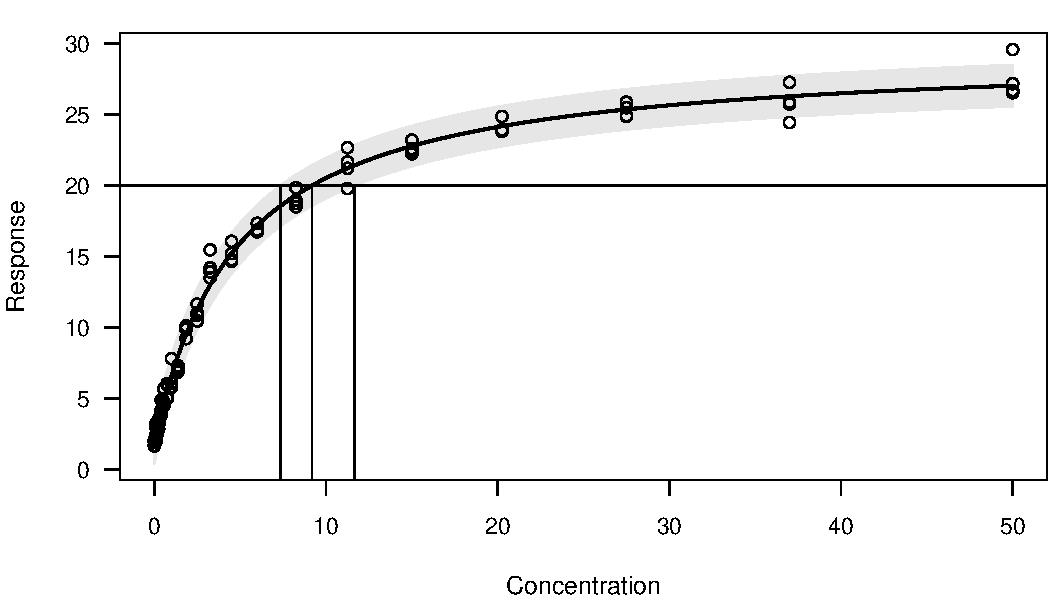
\includegraphics[width=\maxwidth]{figure/elisa-nls} \caption[Four parameter logistic model for the ELISA data]{Nonlinear least squares fit of the ELISA data to the four parameter logistic model with (pointwise) 95\% prediction band.\label{fig:elisa-nls}}
\end{figure}


\end{knitrout}


Figure~\ref{fig:elisa-jags} shows a fitted semiparametric calibration curve, a quadratic \ac{P-spline} with five interior knots. Also shown is the posterior mean based on a fully Bayesian \ac{P-spline} model. Seeing as how the concentration should not be negative, we used a $\mc{U}[0, 50]$ prior for $x_0$, though, lognormal or gamma priors may also be reasonable. The frequentist estimate of $x_0$ is obtained by (numerically) inverting the fitted \ac{P-spline}: $\wh{x}_0 = 9.345$. A (bias-adjusted) inversion interval for $x_0$ based on Equation~\eqref{eqn:bc-inversion-interval} is $(7.462, 11.711)$. As previously mentioned, this interval does not account for the variability of the estimated smoothing parameter $\wh{\sigma}_\epsilon^2/\wh{\sigma}_\alpha^2$, hence, we expect the Bayesian credible interval to be slightly wider. The estimator we use for the Bayesian model is the posterior mode of $x_0$ which is equal to $9.285$. There are a number of ways to compute a 95\% credible interval from a given posterior; for example, \textit{highest posterior density} (HPD) intervals. Here we simply report the 0.025 and 0.975 quantiles of the posterior which are $7.250$ and $11.776$, respectively. As noted earlier, these limits are slightly wider than the corresponding frequentist limits, but this extra wideness is likely due to the added uncertainty of the estimated smoothing parameter. \citet{ori_constructing_1995} also obtained calibration intervals for these data. Their approach involved bootstrapping a cross-validated cubic smoothing spline, but did not account for bias in $\wh{\mu}(x)$. For a brief discussion on bias correction in nonparametric regression using the bootstrap, see \citet[pp. 362-366]{davison_bootstrap_1997}.

\begin{knitrout}
\definecolor{shadecolor}{rgb}{0.969, 0.969, 0.969}\color{fgcolor}\begin{figure}[H]

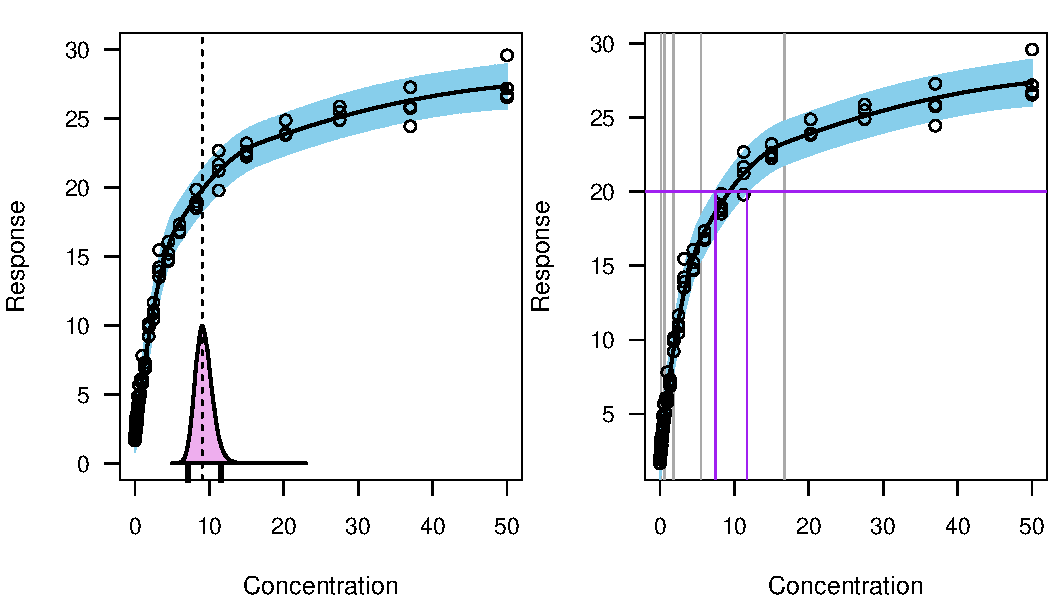
\includegraphics[width=0.9\linewidth]{figure/elisa-jags} \caption[Bayesian nonparametric calibration for ELISA data]{Nonparametric calibration for ELISA data. \textit{Left}: Bayesian \ac{P-spline} with posterior and 95\% credible interval for $x_0$. The shaded blue region represents the (pointwise) prediction band and the density curve represents the posterior of $x_0$. \textit{Right}: Mixed-effects model \ac{P-spline} with bias-adjusted 95\% calibration interval for $x_0$. The shaded blue region represents the (pointwise) bias-adjusted predction band.\label{fig:elisa-jags}}
\end{figure}


\end{knitrout}


\begin{table}[H]
\centering
\caption[Calibration results for the ELISA data]{Point and interval estimates for $x_0$ for the ELISA data with $y_0 = 20$.\label{tab:elisa}}
\begin{tabular}{llc}
  \toprule
  \textbf{Method} & \textbf{Estimate} & \textbf{95\% interval} \\
  \midrule
  Parametric (homoscedastic errors)   & $9.184$ & $(7.356, 11.657)$ \\
  \ac{P-spline} (bias-adjusted)            & $9.345$ & $(7.462, 11.711)$ \\
  \ac{P-spline} (Bayesian)                 & $9.285$ & $(7.250, 11.776)$ \\
  \bottomrule
\end{tabular}
\end{table}

\section{Discussion}
\label{sec:semipar-discussion}
We have proposed a new method for calibration in a semiparametric setting based on the mixed model approach to smoothing that corrects for bias in the smoothed calibration curve. While the idea of using \ac{LMM}s for penalized smoothing is not new (see, for example, \citet[pp. 13 - 17]{demidenko_mixed_2013}), this approach has never been adapted for the calibration problem as we have proposed here. By using a simple Monte Carlo experiment, we have demonstrated that bias-adjusted prediction intervals can be used to (numerically) obtain calibration intervals for the unknown $x_0$ that have good coverage probabilities. We have discussed a situation where this bias-correction is more serious (i.e., regulation, or rather, calibration where the unknown $x_0$ corresponds to some specified mean response $\mu_0$). Finally, we developed a Bayesian framework for semiparametric calibration by extending the approach originally put forth by \citet{hoadley_bayesian_1970} for linear calibration (see Section~\ref{sec:bayesian}). The frequentist framework, while fast and simple, has the same disadvantage inherent in \ac{LMM} inference; that is, the variance of the estimated smoothing parameter (which is a function of the estimated variance components) is ignored. The Bayesian approach handles this by incorporating prior information for all unknown parameters in the model, leading to slightly wider calibration intervals. The Bayesian approach we presented, however, is slower and more difficult to implement in practice.

\subsection{Priors}
Although we used a uniform prior for $x_0$ in our examples, such a prior for $x$ is unlikely to be useful in general and we recommend a more careful elicitation of prior information. A sensitivity analysis should also be carried out to see if the results are sensitive to the choice of prior for $x_0$. Although inverse gamma priors are commonly used in practice as noninformative priors for scale parameters in hierarchical models (e.g., the variance components in a \ac{LMM}), \citet{gelman_prior_2006} argued against their use. Instead, Gelman adovcated the use of conditionally conjugate priors from a new folded-noncentral-$t$ family.

\subsection{Future work}
The methods proposed in this chapter open the door to a number of future research opportunities. Perhaps, the most interesting (and logical) next step would be the inclusion of constraints. For example, we have assumed that the calibration curve is monotonic over the range of interest. Fortunately, this is not usually a concern when the data are collected from a carefully designed experiment. The semiparametric fit, however, is not necessarily monotonic for every value of the smoothing parameter which may cause problems when, say, obtaining a bias-adjusted calibration interval. It is possible, however, to incorporate constraints, such as monotonicity, using the general projection method described in \citet{mammen_general_2001}. Until such a constraint can be smoothly incorporated (no pun intended) into our semiparametric approach to calibration, we can instead rely on inference regarding the first derivative of $f$ as described in \citet[pp. 151-156]{ruppert_semiparametric_2003}. For instance, if we assume that $f$ is monotonically increasing (decreasing) over the interval $[a, b]$, then a plot of the estimated first derivative of the regression function should lie completely above (below) the $x$-axis. This derivative function can be estimated in exactly the same way as the regression function itself, that is, using \ac{P-spline}s. Therefore, a thorough calibration analysis might include a plot of the data with fitted mean response, supplemented by a plot of the estimated first derivative function (possibly with a confidence band). For instance, we might supplement our analysis of the ELISA data with the following graphic:

\begin{knitrout}
\definecolor{shadecolor}{rgb}{0.969, 0.969, 0.969}\color{fgcolor}\begin{figure}[H]

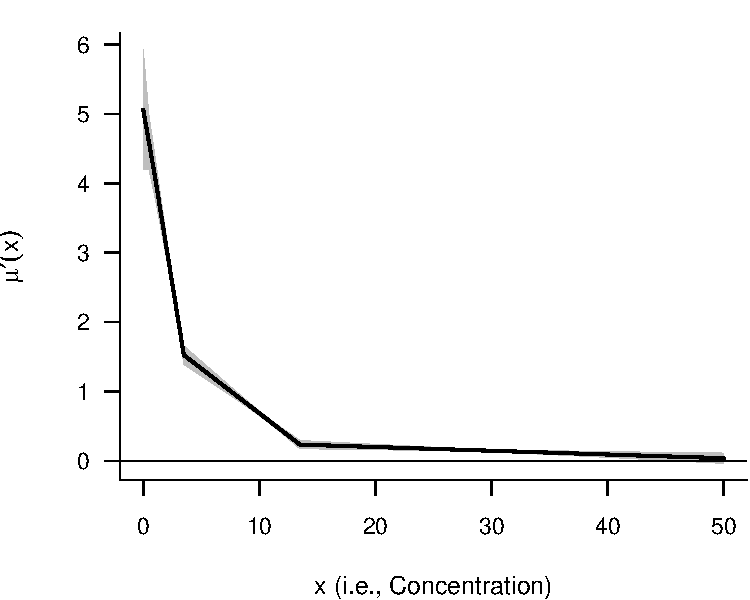
\includegraphics[width=\maxwidth]{figure/derivative-plot} \caption[First derivative plot for the ELISA example]{Estimate of the first derivative of the regression function for the ELISA example with a 95\% global confidence band. A horizontal reference line is displayed at zero on the $y$-axis. This plot was produced using the \code{R} package \pkg{SemiPar}.\label{fig:derivative-plot}}
\end{figure}


\end{knitrout}



%% Calibration with Dependent Data ---------------------------------------------

% !Rnw root = Master.Rnw




\chapter{Calibration with Grouped Data}
\label{chp:cal-dependent}

% \begin{framed}
% \textcolor{magenta}{
% \textbf{TODO:}
% \begin{itemize}
%   \item extend bladder volume data example by adding additional unknowns at 20 $mm^2$ and 90 $mm^2$;
% \end{itemize}
% }
% \end{framed}

In this chapter, we extend the application of calibration to \textit{grouped data}; that is, data in which the observations are grouped into disjoint classes called clusters or groups. Common examples of grouped data include \textit{repeated measures data} and \textit{longitudinal data}. Groups tend to be homogeneous, therefore, observations belonging to the same group cannot be considered independent. (Although, observations between clusters usually are.) Thus, we need to account for within cluster dependence when modeling this type of data. To our knowledge, other than \citet{oman_calibration_1998}, very little has been done for calibration with grouped data. Oman considered a simpler model that only allowed for the intercept and slope to vary between groups, whereas we take a more general (and practical) approach that allows for an arbitrary random effects structure. Furthermore, while Oman considers only one type of calibration interval, we discuss four different calibration intervals that can be computed for grouped data, along with some adjustments to improve their accuracy. Moreover, the calibration interval considered by Oman was based on an approximate parametric bootstrap that did not account for the variance attributed by the random variable $\mc{Y}_0$.

The \ac{LMM} was introduced in Section~\ref{sec:lmms}. In Section~\ref{sec:calibration-lmm-introduction}, we discuss a particular useful LMM: the \textit{random coefficient model}. In Section~\ref{sec:calibration-lmm-point}, we propose a simple method for estimating the unknown $x_0$ in a mixed model setting. We argue the utility of this approach by showing that, in a particular case, it coincides with the \ac{ML} solution. In Sections \ref{sec:calibration-lmm-wald} and \ref{sec:calibration-lmm-inversion}, we discuss construction of Wald and asymptotic inversion intervals, respectively. We then propose a fully parametric bootstrap approach for controlled calibration in Section \ref{sec:calibration-lmm-parboot}. Unlike \citet{oman_calibration_1998}, our parametric bootstrap algorithm does take into account the variability attributed by $\mc{Y}_0$. Distribution-free calibration intervals are (briefly) considered in Section~\ref{sec:calibration-lmm-distfree}. Finally, Section~\ref{sec:bladder-example} applies the aforementioned techniques to a real dataset taken from \citet{brown_measurement_1993}.

\section{LMMs for repeated measures data}
\label{sec:calibration-lmm-introduction}
As discussed in Section~\ref{sec:lmms}, the \ac{LMM} extends the basic \ac{LM} \eqref{eqn:linmod-matrixform} to 
\begin{equation}
\label{eqn:lmm-matrix}
  \bc{Y} = \X\bm{\beta} + \Z\bm{\alpha} + \bm{\epsilon},
\end{equation}
where $\X$ and $\Z$ are known design matrices, $\bm{\beta}$ is a vector of fixed effects, $\bm{\alpha}$ is a vector of random effects, and $\bm{\epsilon}$ is a vector of random errors. Since we are using mixed models to analyze grouped data, it would behoove us to decompress model~\eqref{eqn:lmm-matrix} into the form introduced by \citet{laird_random_1982},
\begin{equation}
\label{eqn:lmm-laird-ware}
  \bc{Y}_i = \X_i\bm{\beta} + \Z_i\bm{\alpha}_i + \bm{\epsilon}_i, \quad i = 1, \dotsc, m,
\end{equation}
where, for the $i$-th group:
\begin{itemize}
  \item $\bc{Y}_i$ is an $n_i \times 1$ vector of response variables;
  \item $\X_i$ and $\Z_i$ are known design matrices of dimensions $n_i \times p$ and $n_i \times q$, respectively;
  \item $\bm{\beta}$ is a $p \times 1$ vector of fixed effects;
  \item $\bm{\alpha}_i$ is a $q \times 1$ vector of random effects;
  \item $\bm{\epsilon}_i$ is an $n_i \times 1$ vector of random errors.
\end{itemize}
Furthermore, it is assumed that the random variables $\big\{\bm{\alpha}_i\big\}_{i=1}^m$ and $\big\{\bm{\epsilon}_i\big\}_{i=1}^m$ are mutually independent and distributed according to
\begin{equation*}
  \bm{\alpha}_i \sim \mc{N}\left(\bm{0}, \bm{G}\right), \quad
  \bm{\epsilon}_i \sim \mc{N}\left(\bm{0}, \sigma_\epsilon^2\bm{R}_i\right).
\end{equation*}
For our purposes, we shall assume that $\bm{R}_i = \bm{I}$ (an $N \times N$ identity matrix); that is, we are assuming constant variance within groups. Also, for computational purposes (e.g., maximizing the likelihood), it is convenient to reparameterize $\bm{G}$ as $\sigma_\epsilon^2\bm{G}^\dagger$, where $\bm{G}^\dagger$ is the ``scaled'' variance-covariance matrix for the random effects. In other words, we have that
\begin{equation*}
  \bm{\alpha}_i \sim \mc{N}\left(\bm{0}, \sigma_\epsilon^2\bm{G}^\dagger\right), \quad
  \bm{\epsilon}_i \sim \mc{N}\left(\bm{0}, \sigma_\epsilon^2\bm{I}\right).
\end{equation*}
Model~\eqref{eqn:lmm-matrix} can also be written in marginal form as
\begin{equation*}
  \bc{Y}_i \sim \mc{N}\left(\X_i\bm{\beta}, \bm{V}_i\right),
\end{equation*}
where 
\begin{equation*}
\bm{V}_i = \Z_i\bm{G}\Z_i\trans + \sigma_\epsilon^2\bm{I}. 
\end{equation*}
In long notation (Equation~\eqref{eqn:lmm-matrix}), we have
\begin{align*}
  \bc{Y} &= \begin{bmatrix} \bc{Y}_1 \\ \vdots \\ \bc{Y}_m \end{bmatrix}_{N \times 1}, \quad
  \X = \begin{bmatrix} \X_1 \\ \vdots \\ \X_m \end{bmatrix}_{N \times p}, \quad
\Z =
  \begin{bmatrix}
    \Z_1 & \bm{0} & \bm{0}   \\
    \bm{0}   & \ddots         & \bm{0}   \\
    \bm{0}   & \bm{0} & \Z_m
  \end{bmatrix}_{N \times mq}, \\
  \bm{\alpha} &= \begin{bmatrix} \bm{\alpha}_1 \\ \vdots \\ \bm{\alpha}_m \end{bmatrix}_{mq \times 1}, \quad 
   \bm{\epsilon} = \begin{bmatrix} \bm{\epsilon}_1 \\ \vdots \\ \bm{\epsilon}_m \end{bmatrix}_{N \times 1},
\end{align*}
% \begin{align*}
%   \bc{Y} = \left(\bc{Y}_i, \dotsc, \bc{Y}_{n_i}\right)\trans, \quad
%   \bm{\alpha} = \left(\bm{\alpha}_1, \dotsc, \bm{\alpha}_m\right)\trans, \quad
%   \bm{\epsilon} = \left(\bm{\epsilon}_1, \dotsc, \bm{\epsilon}_m\right)\trans, \\
%   \X = \Big\{_{c} \X_i \Big\}_{i = 1}^m, \quad
%   \Z = \Big\{_{d} \Z_i \Big\}_{i = 1}^m,
% \end{align*}
  where $N = \sum_{i=1}^m n_i$ is the total number of observations. Similarly, this can be summarized in marginal form as $\bc{Y} \sim \mc{N}\left(\X\bm{\beta}, \bm{V}\right)$ where 
\begin{equation*}
  \bm{V} = \sigma_\epsilon^2\Big\lbrace_{\text{diag }} \bm{I}_{n_i} + \Z_i\bm{G}^\dagger\Z_i\trans \Big\rbrace_{i = 1}^m. 
\end{equation*}  
Notice, in this model, how the fixed effects are used to model the mean of $\bc{Y}$ while the random effects govern the variance-covariance structure of $\bc{Y}$. In fact, as pointed out by \citet{mcculloch_generalized_2008}, a key reason for including random effects in a model is to simplify the otherwise difficult task of dealing with $N(N+1)/2$ unique elements of $\bm{V}$. 

Ignoring constants, the log-likelihood for the data can be written as
\begin{multline}
\label{eqn:lmm-loglik}
  \loglik\left(\bm{\beta}, \sigma_\epsilon^2, \bm{\theta}\right) = -\frac{N}{2}\log(\sigma_\epsilon^2) - \frac{1}{2}\sum_{i = 1}^m\log\left|\bm{I} + \Z_i\bm{G}^\dagger\Z_i\trans\right| \\ - \frac{1}{2\sigma_\epsilon^2}\sum_{i = 1}^m \left(\bc{Y}_i - \X_i\bm{\beta}\right)\trans\left(\bm{I} + \Z_i\bm{G}^\dagger\Z_i\trans\right)^{-1}\left(\bc{Y}_i - \X_i\bm{\beta}\right),
\end{multline}
where $\bm{\theta}$ is a vector containing the unique elements of $\bm{G}^\dagger$. Since $\bm{G}^\dagger$ is symmetric, it has at most $q(q+1)/2$ unique elements; hence, $\bm{\theta}$ has a maximum dimension of $q(q+1)/2$. In many practical applications, however, we can restrict $\bm{G}^\dagger$ (or equivalently $\bm{G}$) to simpler forms involving only a few parameters. For example, $\bm{G}^\dagger$ may be a constant multiple of the identity matrix, $\tau\bm{I}$, which corresponds to uncorrelated random effects with constant variance $\sigma_\epsilon^2\tau$; in this case, $\bm{\theta} = \tau$ has dimension one. This is the variance-covariance structure we used for the random coefficients in the mixed model approach to P-splines in the previous chapter.

One of the most useful LMMs for repeated measures data is the so-called \textit{random linear trend model}:
\begin{equation}
\label{eqn:linear-random-trend}
  \mc{Y}_{ij} = \left(\beta_0 + \alpha_{0i}\right) + \left(\beta_1 + \alpha_{1i}\right)x_{ij} + \epsilon_{ij}, \quad i = 1, \dotsc, m, \quad j = 1, \dotsc, n_i,
\end{equation}
where $\beta_0$ and $\beta_1$ are fixed effects, $\big\{\alpha_{0i}\big\}$ are random intercepts distributed as $\mc{N}\left(0, \sigma_0^2\right)$, $\big\{\alpha_{1i}\big\}$ are random slopes distributed as $\mc{N}\left(0, \sigma_1^2\right)$, and $\big\{\epsilon_{ij}\big\}$ are i.i.d. random errors distributed as $\mc{N}\left(0, \sigma_\epsilon^2\right)$. Also, if we let $\cov\left\{\alpha_{0i}, \alpha_{1i}\right\} = \sigma_{01}$, then 
\begin{equation*}
  \bm{G} = 
    \begin{bmatrix}
      \sigma_0^2  & \sigma_{01} \\
      \sigma_{01} & \sigma_1^2
    \end{bmatrix}.
\end{equation*}
We often assume the random intercepts and slopes are independent, that is, $\sigma_1^2 = 0$; this can be formally tested using a \textit{likelihood ratio test}. Also, setting $\alpha_{01} = \dotsb = \alpha_{0m} = 0$ or $\alpha_{11} = \dotsb = \alpha_{1m} = 0$ yields the \textit{random intercept} and \textit{random slope} models, respectively (see Figure~\ref{fig:random-coefficients}). Considerable simplifications arise for the balanced cases (i.e., when $n_i = n$ for all $i$). For example, for a balanced random intercept model, the matrix $\Z$ of Equation~\eqref{eqn:lmm-matrix} is just $\Z = \bm{I}_m \otimes \bm{1}_n$, where the symbol $\otimes$ denotes the Kronecker product. Estimating the fixed effects and variance components for model~\eqref{eqn:linear-random-trend} is also much simpler in the balanced case. 

\begin{knitrout}
\definecolor{shadecolor}{rgb}{0.969, 0.969, 0.969}\color{fgcolor}\begin{figure}[H]

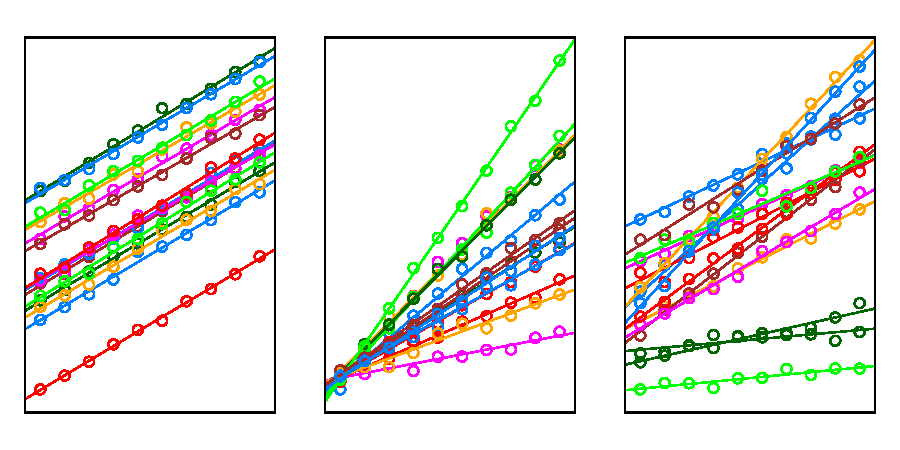
\includegraphics[width=\maxwidth]{figure/random-coefficients} \caption[Common random coefficient models for grouped data]{Common random coefficient models for grouped data. Each plot consists of ten measurements on 15 subjects---each of which has a positive, linear trend. \textit{Left}: Random intercepts. \textit{Middle}: Random slopes. \textit{Right}: Random intercepts and slopes.\label{fig:random-coefficients}}
\end{figure}


\end{knitrout}


\subsection{Prediction of future observations}
In the literature for mixed models, prediction of future observations is often overshadowed by the prediction of random effects. Nonetheless, prediction of future observations in mixed models is an important topic---see \citet{jiang_linear_2007} for some motivating examples. For LMMs, there are two kinds of predictions we can make regarding a future observations: (1) predicting a \emph{new} observation \emph{within} an existing group, and (2) predicting a \emph{new} observation in a \emph{new} group. Since longitudinal studies often aim to make inference for the whole population under study---and not just the groups sampled---we will restrict our attention to case (2). In particular, for calibration, we will assume that a (single) new observation, denoted $\mc{Y}_0$, is independent of the current observations and does not belong to an existing group. 

\section{Point estimation}
\label{sec:calibration-lmm-point}
In this section, we discuss point estimation of $x_0$ in a mixed model setting. Generally, it is difficult to compute the \ac{ML} estimate of $x_0$ due to the complex nature of mixed model likelihoods; however, as shown below, some cases yield relatively simple results. 

Consider the linear random trend model (Equation~\eqref{eqn:linear-random-trend}). For a particular $x$, we have
\begin{equation*}
  \mc{Y} = \underbrace{\strut \beta_0 + \beta_1 x}_\text{\strut FIXED} + \overbrace{\strut \alpha_0 + \alpha_1 x + \epsilon}^\text{\strut RANDOM} = \underbrace{\strut \mu\left(x; \bm{\beta}\right)}_\text{\strut FIXED} + \overbrace{\strut R\left(x; \bm{\alpha}\right)}^\text{\strut RANDOM},
\end{equation*}
where $\mu\left(x; \bm{\beta}\right) = \E\left\{\mc{Y}|x\right\}$ is the (population) mean response. For simplicity of notation, let $\mu\left(x\right) = \mu\left(x; \bm{\beta}\right)$. Solving the equation $\mu(x) = \beta_0 + \beta_1 x$ for $x$, we get (assuming $
\beta_1 \ne 0$)
\begin{equation*}
  x = \frac{\mu(x) - \beta_0}{\beta_1}.
\end{equation*}
If $\mc{Y}_0$ denotes a random observation from a normal distribution with mean $\mu(x_0)$, then $\E\left\{\mc{Y}_0\right\} = \mu(x_0) = \beta_0 + \beta_1 x_0$, therefore, a natural estimator of $x_0$ is
\begin{equation}
\label{eqn:calibration-lmm-mle}
  \wh{x}_0 = \frac{\mc{Y}_0 - \wh{\beta}_0}{\wh{\beta}_1},
\end{equation}
where $\wh{\bm{\beta}} = \left(\wh{\beta}_0, \wh{\beta}_1\right)\trans$ is the \ac{EBLUE} of $\bm{\beta} = \left(\beta_0, \beta_1\right)\trans$. Notice how this has the same form as the classical estimator (Equation~\eqref{eqn:x0-mle}) discussed in Section~\ref{sec:point-estimation}. In fact, for the balanced random intercept model, the classical estimator is still the \ac{ML} estimator of $x_0$; in other words, we can compute the \ac{ML} estimator of $x_0$ using ordinary least squares with i.i.d. normal errors! To see this, note that for the general case $\bm{G}^\dagger = \tau\bm{I}$ and $\Z_i = \bm{1}_i$ (a column vector of all ones), hence, $\bm{V}_i = \sigma_\epsilon^2\left(\bm{I}_i + \tau\bm{1}_i\bm{1}_i\trans\right)$. Therefore, we can write
\begin{equation*}
  \bc{Y}_i \sim \mc{N}\left\{\X_i\bm{\beta}, \sigma_\epsilon^2\left(\bm{I}_i + \tau\bm{1}_i\bm{1}_i\trans\right)\right\}, \quad i = 1, \dotsc, m,
\end{equation*}
where $\X_i$ is an $n_i \times 2$ design matrix with $j$-th row equal to $\X_{ij}\trans = \left(1, x_{ij}\right)$, $\bm{\beta} = \left(\beta_0, \beta_1\right)\trans$ is a vector of fixed effects, $\sigma_\epsilon^2$ is the within-subject variance, and $\sigma_\epsilon^2\tau$ is the variance of the random intercepts. From Equation~\eqref{eqn:lmm-loglik}, the log-likelihood for the data (ignoring constants) is
\begin{multline*}
  \loglik_{\mathrm{I}}\left(\bm{\beta}, \sigma_\epsilon^2, \tau\right) = -\frac{N}{2}\log\left(\sigma_\epsilon^2\right) - \frac{1}{2}\sum_{i = 1}^m \log\left|\bm{I} + \tau\bm{1}_i\bm{1}_i\trans\right| \\ - \frac{1}{2\sigma_\epsilon^2}\sum_{i = 1}^m \left(\bc{Y}_i - \X_i\bm{\beta}\right)\trans\left(\bm{I} + \tau\bm{1}_i\bm{1}_i\trans\right)^{-1}\left(\bc{Y}_i - \X_i\bm{\beta}\right).
\end{multline*}
The subscript ``$\mathrm{I}$'' is there to remind us that this is the likelihood for the standards, the data from the first stage of the calibration experiment (see Section~\ref{sec:intro}). Using the following formulas \citep[pg. 49]{demidenko_mixed_2013},
\begin{itemize}
  \item $\left|\bm{I} + \tau\bm{1}_i\bm{1}_i\trans\right| = 1 + n_i\tau$;
  \item $\left(\bm{I} + \tau\bm{1}_i\bm{1}_i\trans\right)^{-1} = \bm{I} - \frac{\tau}{1 + n_i\tau}\bm{1}_i\bm{1}_i\trans$;
\end{itemize}
the log-likelihood simplifies to
\begin{multline*}
  \loglik_{\mathrm{I}}\left(\bm{\beta}, \sigma_\epsilon^2, \tau\right) = -\frac{N}{2}\log\left(\sigma_\epsilon^2\right) - \frac{1}{2}\sum_{i = 1}^m \log\left(1 + n_i\tau\right) \\ - \frac{1}{2\sigma_\epsilon^2}\sum_{i = 1}^m \left(\bc{Y}_i - \X_i\bm{\beta}\right)\trans\left(\bm{I} - \frac{\tau}{1 + n_i\tau}\bm{1}_i\bm{1}_i\trans\right)\left(\bc{Y}_i - \X_i\bm{\beta}\right).
\end{multline*}
Similarly, the log-likelihood for the (single) unknown (i.e., the log-likelihood for the data from the second stage of the calibration experiment) is 
\begin{equation*}
  \loglik_{\mathrm{II}}\left(\bm{\beta}, \sigma_\epsilon^2, \tau, x_0\right) = -\frac{1}{2}\log\left(\sigma_\epsilon^2\right) - \frac{1}{2}\log\left(1 + \tau\right) - \frac{1}{2\sigma_\epsilon^2\left(1 + \tau\right)}\left(\mc{Y}_0 - \beta_0 - \beta_1 x_0\right)^2.
\end{equation*}
From the independence of $\bc{Y}$ and $\mc{Y}_0$, the log-likelihood for the pooled data, denoted $\loglik\left(\bm{\beta}, \sigma_\epsilon^2, \tau, x_0\right)$, is given by
\begin{align*}
  \loglik\left(\bm{\beta}, \sigma_\epsilon^2, \tau, x_0\right) &= \loglik_{\mathrm{I}}\left(\bm{\beta}, \sigma_\epsilon^2, \tau\right) + \loglik_{\mathrm{II}}\left(\bm{\beta}, \sigma_\epsilon^2, \tau, x_0\right) \\
  &= -\frac{N+1}{2}\log\left(\sigma_\epsilon^2\right) - \frac{1}{2}\sum_{i = 1}^m \log\left(1 + n_i\tau\right) - \frac{1}{2}\log\left(1 + \tau\right) \newln - \frac{1}{2\sigma_\epsilon^2}\sum_{i = 1}^m \left(\bc{Y}_i - \X_i\bm{\beta}\right)\trans\left(\bm{I} - \frac{\tau}{1 + n_i\tau}\bm{1}_i\bm{1}_i\trans\right)\left(\bc{Y}_i - \X_i\bm{\beta}\right) \newln - \frac{1}{2\sigma_\epsilon^2\left(1 + \tau\right)}\left(\mc{Y}_0 - \beta_0 - \beta_1 x_0\right)^2.
\end{align*}
Thus, the full log-likelihood is the sum of two parts: the log-likelihood for the standards, and the log-likelihood for the unknown. Equating to zero the partial derivative of the full log-likelihood with respect to the parameter $x_0$ results in $\widetilde{x}_0\left(\bm{\beta}\right) = \left(\mc{Y}_0 - \beta_0\right)/\beta_1$. In other words, for any value of $\bm{\beta}$, $\widetilde{x}_0\left(\bm{\beta}\right)$ maximizes the likelihood with respect to $x_0$. Plugging this back into the log-likelihood yields the \textit{profiled log-likelihood}
\begin{multline*}
  \loglik_p\left(\bm{\beta}, \sigma_\epsilon^2, \tau\right) = -\frac{N+1}{2}\log\left(\sigma_\epsilon^2\right) - \frac{1}{2}\sum_{i = 1}^m \log\left(1 + n_i\tau\right) - \frac{1}{2}\log\left(1 + \tau\right) \\ - \frac{1}{2\sigma_\epsilon^2}\sum_{i = 1}^m \left(\bc{Y}_i - \X_i\bm{\beta}\right)\trans\left(\bm{I} - \frac{\tau}{1 + n_i\tau}\bm{1}_i\bm{1}_i\trans\right)\left(\bc{Y}_i - \X_i\bm{\beta}\right),
\end{multline*}
Similarly, equating the partial derivative of $\loglik_p\left(\bm{\beta}, \sigma_\epsilon^2, \tau\right)$, with respect to the parameter $\sigma_\epsilon^2$, to zero yields 
\begin{equation*}
  \widetilde{\sigma}_\epsilon^2\left(\bm{\beta}, \tau\right) = \frac{1}{N + 1}\sum_{i = 1}^m \left(\bc{Y}_i - \X_i\bm{\beta}\right)\left(\bm{I} - \frac{\tau}{1 + n_i\tau}\bm{1}_i\bm{1}_i\trans\right)\left(\bc{Y}_i - \X_i\bm{\beta}\right)\trans.
\end{equation*}
Substituting this back into the profiled log-likelihood and simplifying (i.e., cancelling common factors and ignoring constants) we get
\begin{multline*}
  \loglik_p\left(\bm{\beta}, \tau\right) = -\frac{N+1}{2}\log\left\{\sum_{i = 1}^m \left(\bc{Y}_i - \X_i\bm{\beta}\right)\trans\left(\bm{I} - \frac{\tau}{1 + n_i\tau}\bm{1}_i\bm{1}_i\trans\right)\left(\bc{Y}_i - \X_i\bm{\beta}\right)\right\} \\ - \frac{1}{2}\sum_{i = 1}^m \log\left(1 + n_i\tau\right) - \frac{1}{2}\log\left(1 + \tau\right),
\end{multline*}
The parameters $x_0$ and $\sigma_\epsilon^2$ have been ``profiled out'', resulting in a simpler log-likelihood in only $p + 1$ parameters. We could continue in this fashion with the parameter $\bm{\beta}$ as well, although it is quite easy to see that the value of $\bm{\beta}$ that maximizes $\loglik_p\left(\bm{\beta}, \tau\right)$ is just the usual \ac{GLS} estimator, $\widetilde{\bm{\beta}}$, given by Equation~\eqref{eqn:beta-gls}. Furthermore, it can be shown \citep{demidenko_mixed_2013} that, for the balanced case, $\widetilde{\bm{\beta}}$ does not depend on $\tau$ and in fact reduces to the ordinary \ac{LS} estimator $\wh{\bm{\beta}} = \left(\X\trans\X\right)^{-1}\X\trans\bc{Y}$. Thus, the \ac{ML} estimator of $x_0$ for the balanced random intercept model is simply
\begin{equation*}
  \wh{x}_0 = \widetilde{x}_0\left(\wh{\bm{\beta}}\right) = \frac{\mc{Y}_0 - \wh{\beta}_0}{\wh{\beta}_1},
\end{equation*}
where 
\begin{equation*}
  \wh{\beta}_1 = \frac{\sum_{i=1}^n\sum_{j=1}^m\left(x_{ij}-\bar{x}\right)\left(y_{ij}-\bar{y}\right)}{\sum_{i=1}^n\sum_{j=1}^m\left(x_{ij}-\bar{x}\right)^2}, \quad \wh{\beta}_0 = \bar{y} - \wh{\beta}_1\bar{x}.
\end{equation*}

In general, the \ac{ML} estimator $\wh{x}_0$ of $x_0$ is difficult to obtain analytically. For example, in a random slope model, $\mc{Y}_0 \sim \mc{N}\left(\beta_0 + \beta_1 x_0, x_0^2\sigma_\alpha^2 + \sigma_\epsilon^2\right)$, thus, the unknown $x_0$ affects both the mean and variance of $\mc{Y}_0$. A reasonable, and more practical approach, is to proceed as before, that is, by solving the equation $y_0 = \mu(x_0)$ for the unknown $x_0$. As shown above, for the balanced random intercept model, this leads to the \ac{ML} estimate.

We should point out that, in general, the \ac{EBLUE} of $\bm{\beta}$ (Equation~\eqref{eqn:beta-egls}) depends on the estimated variance components through $\wh{\bm{V}}$. Furthermore, recall that for the linear calibration problem, the bias-adjusted \ac{ML} estimator of $\sigma_\epsilon^2$ (the only variance component) is 
\begin{equation}
\label{eqn:mse-mle}
  \wh{\sigma}_\epsilon^2 = \frac{1}{n-2}\sum_{i=1}^n\left(\mc{Y}_i-\wh{\beta}_0-\wh{\beta}_1 x_i\right)^2 + \frac{1}{m-1}\sum_{i=n+1}^{n+m}\left(\mc{Y}_i-\overline{\mc{Y}}_0\right)^2.
\end{equation}
The first term in Equation~\eqref{eqn:mse-mle} is the usual unbiased estimator of $\sigma_\epsilon^2$, and the second term is just the sample variance of the $m$ unknowns $\mc{Y}_{01}, \dotsc, \mc{Y}_{0m}$. If there is only one unknown, then the second term in Equation~\eqref{eqn:mse-mle} is zero! Hence, for a single unknown, the \ac{ML} estimator of the variance $\sigma_\epsilon^2$ (adjusted for bias) is unaffected. We could extrapolate by making a similar argument for calibration in mixed models. That is, if only a single observation, $\mc{Y}_0$, is available from the second stage of the calibration experiment, then the \ac{ML} estimates of the variance components (adjusted for bias) should be unaffected---this would not be the case for replicate unknowns sharing a single unknown $x_0$. In this chapter, we only concern ourselves with the case of a single unknown; thus, we make the argument that the usual estimates of the variance components are valid for calibration inference. 

For illustration, we generated $n = 30$ observations for each of $m = 15$ groups from a random intercept model with fixed effects $\bm{\beta} = \left(0, 1\right)\trans$ and variance components $\sigma_\alpha^2 = 0.01$ and $\sigma_\epsilon^2 = 0.001$. A spaghetti plot of the data is shown in Figure~\ref{fig:simdata-scatter}; notice the apparent linear trend with varying intercepts. For a new observation, $y_0 = 0.75$, the estimate of the corresponding unknown $x_0$ is $\wh{x}_0 = \left(0.75 - \wh{\beta}_0\right)/\wh{\beta}_1 = 0.7819$. Since these data are balanced, $\wh{x}_0$ is also the \ac{ML} estimate of $x_0$. 

\begin{knitrout}
\definecolor{shadecolor}{rgb}{0.969, 0.969, 0.969}\color{fgcolor}\begin{figure}[H]

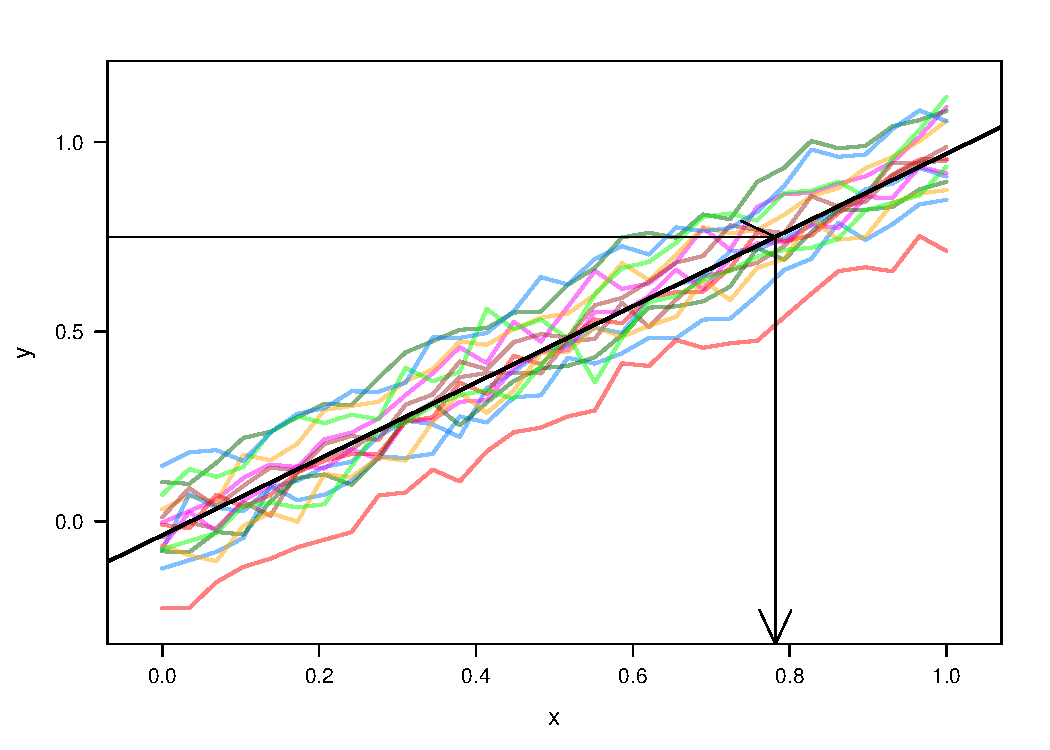
\includegraphics[width=\maxwidth]{figure/simdata-scatter} \caption[Scatterplot of simulated random intercept data]{Simulated random intercept data.\label{fig:simdata-scatter}}
\end{figure}


\end{knitrout}


\section{Wald interval}
\label{sec:calibration-lmm-wald}
The delta method provides the simplest approach to computing confidence intervals, as long as the quantity of interest is a function of random variables that are at least asymptotically normal. Under mild regularity conditions often satisfied in practice, the \ac{ML} estimator $\wh{\bm{\beta}}$ of $\bm{\beta}$ is consistent and asymptotically normal with mean vector $\bm{\beta}$ and asymptotic variance-covariance matrix $\left(\X\trans\bm{V}^{-1}\X\right)^{-1}$ \citep{pinheiro_topics_1994}. Furthermore, by assumption, $\mc{Y}_0$ is distributed as $\mc{N}\left(\beta_0 + \beta_1 x_0, \sigma_0^2\right)$, where $\sigma_0^2$ denotes the variance of $\mc{Y}_0$ which, depending on the random effects structure of the model, may involve the unknown $x_0$. For instance, if $R\left(x; \bm{\alpha}\right) = \alpha + \epsilon$ (i.e., a random intercept model), then $\sigma_0^2 = \sigma_\alpha^2 + \sigma_\epsilon^2$, whereas if $R\left(x; \bm{\alpha}\right) = \alpha x + \epsilon$ (i.e., a random slope model), then $\sigma_0^2 = x_0^2\sigma_\alpha^2 + \sigma_\epsilon^2$ which depends on $x_0$. Although our attention is restricted to LMMs in this dissertation, the simplicity of the Wald-based approach extends to nonlinear mixed-effects models (NLMMs) as well. For an introduction to NLMMs, see \citet{pinheiro_topics_1994} and \citet{pinheiro_mixed_2009}.

The Wald statistic, denoted $\mc{W}$, is essentially a generalization of the usual $\mc{Z}$-statistic. Here it is the point estimator, normalized by an estimate of its standard error which we obtain using Taylor's theorem. By assumption, for large enough $N$, $\mc{W} = \wh{x}_0^2/\wh{\var}\left\{\wh{x}_0\right\}$ has a $\chi^2(1)$ distribution. As pointed out by \citet[p. 184]{harrell_regression_2001}, most statistical packages treat $\sqrt{\mc{W}}$ as having a $t$-distribution  with degrees of freedom $df$ (rather than a standard normal distribution), however, there is usually no basis for this outside of the ordinary linear model \citep{gould_confidence_1993}.

We discussed the delta method for calibration in Section~\ref{sec:wald_int}, where we used a first-order Taylor series expansion to approximate the variance of $\wh{x}_0$. The same basic procedure holds here for LMMs except now $\var\left\{\mc{Y}_0\right\}$ contains additional variability attributed by the random effects. As a simple example, we consider the balanced random intercept model. For this case, we have shown that the \ac{ML} estimator of $x_0$ is given by $\wh{x}_0 = \left(\mc{Y}_0 - \wh{\beta}_0\right)/\wh{\beta}_1$. We should make clear, however, that even though $\wh{\bm{\beta}}$ does not depend on the variance components, its variance-covariance matrix does! Therefore, we still need to compute the variance-covariance matrix of $\wh{\bm{\beta}}$ from a mixed model; for example, the variance-covariance matrix obtained from the \code{SAS/STAT} \citep{sas_program} software's \code{PROC MIXED} procedure or the \code{lme} function from the \code{R} package \pkg{nlme} \citep{pinheiro_nlme_2013}. The variance-covariance matrix of $\left(\mc{Y}_0, \wh{\bm{\beta}}\right)$ is
\begin{equation}
\label{eqn:Sigma}
\Sigma = \begin{bmatrix}
           \var\left\{\mc{Y}_0\right\} & \bm{0} \\
           \bm{0} & \var\left\{\wh{\bm{\beta}}\right\}
         \end{bmatrix} = \begin{bmatrix}
           \sigma_0^2 & \bm{0} \\
           \bm{0} & \left(\X\trans\bm{V}^{-1}\X\right)^{-1}
         \end{bmatrix},
\end{equation} 
Since $\mc{Y}_0$ is independent of $\bc{Y}$, it is also independent of $\wh{\bm{\beta}}$. Recall that our point estimate has the form $x = \mu^{-1}\left(y; \bm{\beta}\right)$. Let $\mu_1^{-1}\left(y; \bm{\beta}\right)$ and the vector-valued function $\mu_2^{-1}\left(y; \bm{\beta}\right)$ be the partial derivatives of $\mu^{-1}$ with respect to the parameters $y$ and $\bm{\beta}$, respectively. Our point estimator is given by $\mu^{-1}\left(\mc{Y}_0; \wh{\bm{\beta}}\right)$, where $\mc{Y}_0$ is a new observation and $\wh{\bm{\beta}}$ is the \ac{EBLUE} of $\bm{\beta}$. Using a first-order Taylor-series expansion, an approximate variance for $\wh{x}_0$ is given by
\begin{equation}
\label{eqn:cal-lmm-approx}
  \var\left\{\wh{x}_0\right\} = \left[\mu_1^{-1}\left(\mc{Y}_0; \wh{\bm{\beta}}\right)\right]^2\sigma_0^2 + \left[\mu_2^{-1}\left(\mc{Y}_0; \wh{\bm{\beta}}\right)\right]\trans\left(\X\trans\bm{V}^{-1}\X\right)^{-1}\left[\mu_2^{-1}\left(\mc{Y}_0; \wh{\bm{\beta}}\right)\right].
\end{equation}
Of course, to obtain $\wh{\var}\left\{\wh{x}_0\right\}$, we need to replace $\sigma_0^2$ and $\bm{V}$ in Equation~\eqref{eqn:cal-lmm-approx} with their corresponding estimates $\wh{\sigma}_0^2$ and $\wh{\bm{V}}$, respectively. Once we have $\wh{\var}\left\{\wh{x}_0\right\}$, an approximate $100(1-\alpha)\%$ confidence interval for $\wh{x}_0$ is given by $\wh{x}_0 \pm z_{1-\alpha/2}\sqrt{\wh{\var}\left\{\wh{x}_0\right\}}$.

As pointed out by \citet[p. 283]{davidian_nonlinear_1995}, the first term in Equation~\eqref{eqn:cal-lmm-approx} usually (but not necessarily) dominates the second term, leaving the cruder approximation $\var\left\{\wh{x}_0\right\} = \left[\mu_1^{-1}\left(\mc{Y}_0; \wh{\bm{\beta}}\right)\right]^2\sigma_0^2$. For example, consider the random intercept model discussed earlier. For this model, we have
\begin{align*}
  \mu^{-1}\left(y; \bm{\beta}\right) &= \left(y - \beta_0\right)/\beta_1, \\
  \frac{\partial}{\partial y}\mu^{-1}\left(y; \bm{\beta}\right) &= 1/\beta_1,
\end{align*}
thus, for the balanced case, the crude approximation turns out to be $\var_\mathrm{crude}\left\{\wh{x}_0\right\} = \sigma_\epsilon^2\left(1 + \tau\right)/\wh{\beta}_1^2$. In general, the approximate variance (Equation~\eqref{eqn:cal-lmm-approx}) can be difficult to compute by hand leading to widespread use of the cruder formula. However, given the ease with which complex computations can be carried out numerically (and with great accuracy), it is good practice to compute and use both terms. In Section~\ref{sec:bladder-example}, we illustrate with a real data example how easily this can be done using the software \code{R} (in particular, see Example~\ref{bladder-wald}).

For the simulated data in Figure~\ref{fig:simdata-scatter}, we get an approximate standard error (i.e., using Taylor's theorem) of $0.1$ which produces a Wald-based calibration interval for $x_0$ of $(0.5859, 0.9778)$. Compare this to the cruder interval $(0.5915, 0.9722)$ obtained by using $\var_\mathrm{crude}\left\{\wh{x}_0\right\}$ in place of the full Taylor-series estimate \eqref{eqn:cal-lmm-approx}.

Unfortunately, one of the difficulties with inference in LMMs is that 
\begin{equation*}
  \var\left\{\wh{\bm{\beta}}\right\} = \left(\X\trans\wh{\bm{V}}^{-1}\X\right)  
\end{equation*}  
involves $\wh{\bm{V}}$, but does not take into account its variability. In other words, $\var\left\{\wh{\bm{\beta}}\right\}$ underestimates the true variance of $\wh{\bm{\beta}}$ (see, for example, \citet[pp. 165-167]{mcculloch_generalized_2008}). Thus, any inference relying on $\var\left\{\wh{\bm{\beta}}\right\}$, including the Wald interval for calibration just discussed, may be misleading. An alternative is to use the so-called \textit{parametric bootstrap} to compute a bootstrap estimate of the variance-covariance matrix $\wh{\bm{\beta}}$ to use in place of $\var\left\{\wh{\bm{\beta}}\right\}$ in Equation~\eqref{eqn:Sigma} (see steps (1)-(4) of Algorithm~\ref{alg:parboot_cal} on page~\pageref{alg:parboot_cal}). 

\section{Inversion interval}
\label{sec:calibration-lmm-inversion}
We can also obtain a confidence interval for the unknown $x_0$ by inverting an asymptotic prediction interval for $\mc{Y}_0$. Let $\X_0$ have the same form as the $i$-th row of $\X$, but with $x_{ij}$ replaced with $x_0$. For example, if $\mu\left(x_{ij}; \bm{\beta}\right) = \beta_0 + \beta_1 x_{ij} + \beta_2 x_{ij}^2$, then $\X_0 = \left(1, x_0, x_0^2\right)\trans$. 

For brevity, let $\mu_0 = \mu\left(x_0; \bm{\beta}\right)$, $\widetilde{\mu}_0 = \mu\left(x_0; \widetilde{\bm{\beta}}\right)$, and $\wh{\mu}_0 = \mu\left(x_0; \wh{\bm{\beta}}\right)$ where, as before, $\widetilde{\bm{\beta}}$ and $\wh{\bm{\beta}}$ denote the \ac{BLUE} and \ac{EBLUE} of $\bm{\beta}$, respectively. A new observation, $\mc{Y}_0$ say, with unknown $x_0$, is distributed as $\mc{N}\left(\mu_0, \sigma_0^2\right)$. Clearly, $\mc{Y}_0 - \widetilde{\mu}_0$ is a normally distributed random variable with expectation zero (since $\E\left\{\mc{Y}_0\right\} = \E\left\{\widetilde{\mu}_0\right\} = \mu_0$). Also, note that $\mc{Y}_0$ and $\widetilde{\mu}_0$ are independent, hence, $\cov\left\{\mc{Y}_0, \widetilde{\mu}_0\right\} = 0$. It therefore follows that the statistic 
\begin{equation}
\label{eqn:lmm-predictive-pivot}
  \mc{Z} = \frac{\mc{Y}_0 - \widetilde{\mu}_0}{\sqrt{\var\left\{\mc{Y}_0\right\} + \var\left\{\widetilde{\mu}_0\right\}}} = \frac{\mc{Y}_0 - \widetilde{\mu}_0}{\sqrt{\sigma_0^2 + \X_0\trans\left(\X\trans\bm{V}^{-1}\X\trans\right)^{-1}\X_0}}
\end{equation}
is a \textit{pivotal quantity} that has an asymptotic standard normal distribution or, equivalently, $\mc{Z}^2 \stackrel{\cdot}{\sim} \chi_1^2$ (a Chi-squared distribution with a single degree of freedom). The key here is that $\widetilde{\mu}_0$ is a linear function of $\bc{Y}$. For example, for a balanced random intercept model, Equation \eqref{eqn:lmm-predictive-pivot} reduces to
\begin{equation*}
  \mc{Z} = \frac{\mc{Y}_0 - \widetilde{\beta}_0 - \widetilde{\beta}_1 x_0}{\sqrt{\sigma_\epsilon^2 + \sigma_\alpha^2 + \X_0\trans\left[\X\trans\left( \sigma_\alpha^2\bm{I}_m \otimes \bm{J}_n + \sigma_\epsilon^2\bm{I}_N \right)^{-1}\X\right]^{-1}\X_0}},
\end{equation*}
where $\bm{J}_n = \bm{1}_n\bm{1}_n\trans$ is an $n \times n$ vector of all ones.

In practice, $\sigma_0^2$, $\bm{V}$, and $x_0$ are usually unknown and need to be estimated from the data. In such cases, an approximate pivot (essentially a Wald statistic), denoted $\mc{Q}$, can be obtained by replacing $\sigma_0^2$, $\bm{V}$, and $x_0$ in the above equation with their respective estimates $\wh{\sigma}_0^2$, $\wh{\bm{V}}$, and $\wh{x}_0$. This suggests an approximate $100(1-\alpha)\%$ confidence interval for $x_0$ of
\begin{equation}
\label{eqn:cal-lmm-inversion}
  %\wh{\mc{J}}_\mathrm{cal}(x) = \left\{ x: \mc{Q}^2 \le z_{1-\alpha/2}^2 \right\},
  \wh{\mc{J}}_\mathrm{cal}(x) = \left\{ x: z_{\alpha/2} < \mc{Q} < z_{1-\alpha/2} \right\},
\end{equation}
where $z_{\alpha/2} = z_{1-\alpha/2}$ denote the $\alpha/2$ and $1 - \alpha/2$ quantiles of a standard normal distribution, respectively. Similar to the approximate predictive pivot (Equation~\eqref{eqn:approximate-predictive-pivot}), it is unlikely that Equation~\eqref{eqn:cal-lmm-inversion} will yield closed-form solutions, thus, the solution must be obtained numerically. For the simulated data example, a 95\% inversion interval based on Equation~\eqref{eqn:cal-lmm-inversion}, corresponding to $y_0 = 0.75$, is given by $(0.5859, 0.9779)$, which is very similar to the Wald-based intervals obtained earlier.

\section{Parametric bootstrap}
\label{sec:calibration-lmm-parboot}
In Section~\ref{sec:boot_int}, we discussed how to calculate calibration intervals based on the nonparametric bootstrap. A crucial assumption for the ordinary nonparametric bootstrap, however, is that the data are independent; for reasons discussed earlier, this assumption is typically not valid for grouped data. Nonetheless, a different kind of bootstrap, called the \textit{parametric bootstrap}, has shown promise as a serious inferential tool. For examples, see \citet[pg. 342]{mcculloch_generalized_2008} and \citet{efron_bootstrap_2011}. When applicable, the parametric bootstrap typically gives answers similar to a Bayesian analysis with uninformative priors, however, it is much faster than MCMC simulations (bootstrap simulations usually only require a few thousand iterations whereas traditional MCMC simulations may require tens, or even hundreds of thousands, of iterations). The parametric bootstrap essentially entails sampling from the fitted model itself, rather than sampling (with replacement) from the data. For controlled calibration in a mixed model setting, we propose the following algorithm (essentially a parametric version of Algorithm~\ref{alg:boot_cal} based on the \ac{LMM} instead of the ordinary LM):

\begin{algorithm}[H]
\begin{singlespace}
\SetAlgoNoLine
\For{$r = 1$ \KwTo $R$}{
\begin{enumerate}[(1)]
  \item generate $q$ new values of the random effects, denoted $\bm{\alpha}_r^\boot$, from a $\mc{N}\left(\bm{0}, \wh{\bm{G}}\right)$ distribution; 
  \item generate $N$ new errors, denoted $\bm{\epsilon}_r^\boot$, from a $\mc{N}\left(\bm{0}, \wh{\sigma}_\epsilon^2\bm{I}\right)$ distribution;
  \item set $\bm{y}_r^\boot = \X\wh{\bm{\beta}} + \Z\bm{\alpha}_r^\boot + \bm{\epsilon}_r^\boot$;
  \item update the original model using $\bm{y}_r^\boot$ as the response vector to obtain $\wh{\bm{\beta}}_r^\boot$;
  \item generate $y_{0r}^\boot$ from a $\mc{N}\left(y_0, \wh{\sigma}_0^2\right)$ distribution;
  \item compute $\wh{x}_{0r}^\boot = \mu^{-1}\left(y_{0r}^\boot; \wh{\bm{\beta}}_r^\boot\right)$.
\end{enumerate}
}
\end{singlespace}
\caption{Parametric bootstrap for controlled calibration in LMMs. \label{alg:parboot_cal}}
\end{algorithm}

Note that only steps (5) and (6) are specific to calibration. Similar parametric bootstrap schemes have also been proposed for mixed models. For example, we can condition on the current values of the random effects by ignoring step (1) of Algorithm~\ref{alg:parboot_cal} and using the current \ac{EBLUP}, $\wh{\bm{\alpha}}$, in place of $\bm{\alpha}^\boot$. Semiparametric variants of Algorithm~\ref{alg:parboot_cal} that involve sampling directly from the \ac{EBLUP} and residuals have also been proposed, but \citet{morris_blups_2002} considers this to be bad practice because it consistently underestimates the true variation in the data.




We applied Algorithm~\ref{alg:parboot_cal} to the simulated data from Figure~\ref{fig:simdata-scatter}. A histogram of the $R = 9,999$ bootstrap replicates of $\wh{x}_0$ is shown in Figure~\ref{fig:simdata-parboot-hist}. Not surprisingly, the distribution is reasonably symmetric and approximately normal; the normal Q-Q plot also confirms this. These bootstrap replicates were used to produce the last two confidence intervals in Table~\ref{tab:simdata-intervals}. For comparison, we have also included the calibration intervals computed in the previous sections. The results are all very similar and there is little reason here for choosing one interval over another. The Wald-based intervals are symmetric, but, as can be seen from Figure~\ref{fig:simdata-parboot-hist}, symmetry is not unrealistic for this example (this is not the case for the example given in the next section). The inversion interval is not symmetric about $\wh{x}_0$, as well as the bootstrap intervals, however, the bootstrap approach has the advantage of providing an estimate of the entire sampling distribution of $\wh{x}_0$. It should be noted, though, that the parametric bootstrap assumes that the model specified for the data is correct! If, however, the data were not normal, then all of these intervals would likely produce misleading results. In the next section, we discuss a potential remedy that can be used for non-Gaussian LMMs, that is, LMMs that do not assume a specific distribution for the random effects or the errors.

\begin{knitrout}
\definecolor{shadecolor}{rgb}{0.969, 0.969, 0.969}\color{fgcolor}\begin{figure}[!htb]

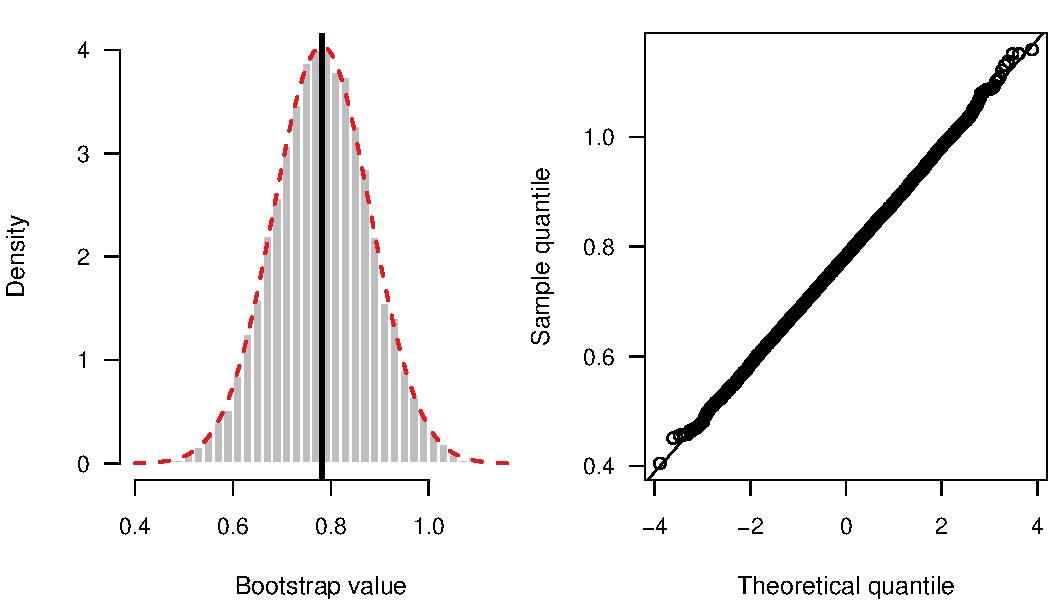
\includegraphics[width=\maxwidth]{figure/simdata-parboot-hist} \caption[Bootstrap distribution of $\wh{x}_0$ for the simulated random intercept data]{Bootstrap distribution of $\wh{x}_0$ obtained using Algorithm~\ref{alg:parboot_cal}. The dotted red curve represents a normal distribution  with mean $\wh{x}_0$ and standard deviation estimated from the bootstrap replicates $\wh{x}_{0r}^\boot$. The vertical black line indicates the position of $\wh{x}_0$.\label{fig:simdata-parboot-hist}}
\end{figure}


\end{knitrout}


\begin{table}[!htb]
\centering
\caption[ 95\% calibration intervals for simulated balanced random intercept data]{Approximate 95\% calibration intervals for the simulated balanced random intercept example. The intervals based on the parametric bootstrap are labeled (PB). \label{tab:simdata-intervals}}
\begin{tabular}{lccccc}
    \toprule
    Interval        & Estimate & Lower 2.5\% & Upper 97.5\% & Length & SE \\
    \midrule
    Wald            & 0.7819 & 0.5859 & 0.9778 & 0.3920 & 0.0999 \\
    Crude interval  & 0.7819 & 0.5915 & 0.9722 & 0.3807 & 0.0971 \\
    Inversion       & 0.7819 & 0.5859 & 0.9779 & 0.3920 & NA     \\
    Normal (PB)     & 0.7819 & 0.5873 & 0.9742 & 0.3870 & 0.0987 \\
    Percentile (PB) & 0.7819 & 0.5895 & 0.9789 & 0.3893 & 0.0987 \\
    \bottomrule
\end{tabular}
\end{table}

% \subsection{\textbf{Parametric bootstrap adjusted Wald interval}}
\subsection{Parametric bootstrap adjusted inversion interval}
Although we favor the bootstrap confidence intervals obtained directly from the $R$ bootstrap replicates of $\wh{x}_0$, researchers are likely more familiar with the inversion and Wald-based intervals discussed in the previous two sections. These intervals, however, use the quantiles from a standard normal distribution (i.e., rely on normal approximations). The parametric bootstrap can be used to improve upon these intervals by replacing the standard normal quantiles with more accurate ones. For instance, for the inversion interval, at each run in Algorithm~\ref{alg:parboot_cal}, we compute
\begin{equation*}
  \mc{Q}^\boot = \frac{y_0^\boot - \mu\left(\wh{x}_0; \wh{\bm{\beta}}^\boot\right)}{\sqrt{\wh{\sigma}_0^{2\boot} + \X_0\trans\left(\X\trans\wh{\bm{V}}^{*-1}\X\trans\right)^{-1}\X_0}},
\end{equation*}
where the denominator is evaluated at $x_0 = \wh{x}_0$. As a result, we obtain the $R$ bootstrap values $\mc{Q}_r^\boot$. Let $\gamma_{\alpha/2}^\boot$ and $\gamma_{1-\alpha/2}^\boot$ denote the sample $\alpha/2$ and $1-\alpha/2$ quantiles of $\mc{Q}_r^\boot$, respectively. A bootstrap adjusted inversion interval for $x_0$ is then given by
\begin{equation}
\label{eqn:cal-lmm-inversion-boot}
  %\wh{\mc{J}}_\mathrm{cal}(x) = \left\{ x: \mc{Q}^2 \le z_{1-\alpha/2}^2 \right\},
  \wh{\mc{J}}_\mathrm{cal}^\boot(x) = \left\{ x: \gamma_{\alpha/2}^\boot < \mc{Q} < \gamma_{1-\alpha/2}^\boot \right\}.
\end{equation}
We illustrate this on the bladder volume example in Section~\ref{sec:bladder-example}. A similar adjustment can also be made for the Wald-based interval as well; this is very similar to the studentized bootstrap procedure outlined in steps (6)-(7) of Algorithm~\ref{alg:boot_cal}.

\section{Distribution free calibration interval}
\label{sec:calibration-lmm-distfree}
For certain cases, we can easily obtain an asymptotic prediction interval for a future observation that does not require normality for the random effects or errors. These intervals are called \textit{distribution-free} prediction intervals; for details, the interested reader is pointed to \citet{jiang_distribution_2002} or \citet{jiang_linear_2007}. This suggests the possibility of a distribution-free calibration interval for $x_0$ by inverting a corresponding distribution-free prediction interval.

We consider only the case of \textit{standard} LMMs. Following \citet{jiang_distribution_2002} and \citet{jiang_linear_2007}, an \ac{LMM} is said to be standard if each $\Z_i$ of Equation~\eqref{eqn:lmm-laird-ware} consists of only 0's and 1's, such that each row contains exactly one 1 and each column has at least one 1. The random intercept model (balanced or unbalanced case) is standard in this sense; the random slope model, however, is not. 

The method for standard LMMs turns out to be quite simple. Compute the ordinary \ac{LS} estimate $\wh{\bm{\beta}} = \left(\X\trans\X\right)^{-1}\X\trans\bm{y}$, then obtain the residual vector as $\bm{e} = \bm{y} - \X\wh{\bm{\beta}}$. Denote the $\alpha/2$ and $1-\alpha/2$ quantiles of the residuals as $e_{\alpha/2}$ and $e_{1-\alpha/2}$, respectively. Then, a distribution-free prediction interval for a new observation, $y_0$, with asymptotic coverage probability $1-\alpha$ is given by
$\left[\wh{\mu}(x_0) + e_{\alpha/2}, \wh{\mu}(x_0) + e_{1-\alpha/2}\right]$, where $\wh{\mu}(x_0)$ is the empirical best predictor of $y_0$. For example, for a random intercept model, the interval in question is simply $\left(\wh{\beta}_0 + \wh{\beta}_1 x_0 + e_{\alpha/2}, \wh{\beta}_0 + \wh{\beta}_1 x_0 + e_{1-\alpha/2}\right)$. If $y_0$ is observed and $x_0$ is the unknown, then this formula can be inverted (in closed-form) to produce an asymptotic $100(1-\alpha)\%$ distribution-free confidence interval for $x_0$ of
\begin{equation} 
\label{eqn:simdata-x0-df}
  \left[ \frac{\left(y_0 - e_{1-\alpha/2}\right) - \wh{\beta}_0}{\wh{\beta}_1}, \frac{\left(y_0 - e_{\alpha/2}\right) - \wh{\beta}_0}{\wh{\beta}_1} \right].
\end{equation}
Using Equation~\eqref{eqn:simdata-x0-df}, a 95\% distribution-free calibration interval for the simulated random intercept example is $(0.6121, 0.9852)$. However, since these data are normal (we know because we generated the data), the intervals given in Table~\ref{tab:simdata-intervals} are probably more accurate. 

\section{Simulation study}
\label{sec:simulation-study}
To illustrate the practical performance of the confidence interval procedures discussed in Sections~\ref{sec:calibration-lmm-wald}-\ref{sec:calibration-lmm-parboot}, we ran a small simulation study in which $\left(x_{ij}, \mathcal{Y}_{ij}\right)$, $i = 1, 2, \dotsc, 30$, $j = 1, 2, \dotsc, 20$, were generated from both
\begin{equation*}
  \mathcal{Y}_{ij} = \left(\alpha_{0j} + \beta_0\right) + \left(\alpha_{1j} + \beta_1\right)x_{ij} + \epsilon_{ij}
\end{equation*}
and
\begin{equation*}
  \mathcal{Y}_{ij} = \left(\alpha_{0j} + \beta_0\right) + \left(\alpha_{1j} + \beta_1\right)x_{ij} + \beta_2 x_{ij}^2 + \epsilon_{ij}.
\end{equation*}
In the first model, $\left(\beta_0, \beta_1\right) = \left(0, 2\right)$, $\alpha_{0j} \stackrel{iid}{\sim} \mathcal{N}\left(0, 0.001\right)$, $\alpha_{1j} \stackrel{iid}{\sim} \mathcal{N}\left(0, 0.05\right)$, and $\epsilon_{ij} \stackrel{iid}{\sim} \mathcal{N}\left(0, 0.001\right)$. Similarly, in the second model, $\left(\beta_0, \beta_1, \beta_2\right) = \left(0, 3, -1\right)$, $\alpha_{0j} \stackrel{iid}{\sim} \mathcal{N}\left(0, 0.0001\right)$, $\alpha_{1j} \stackrel{iid}{\sim} \mathcal{N}\left(0, 0.05\right)$, and $\epsilon_{ij} \stackrel{iid}{\sim} \mathcal{N}\left(0, 0.001\right)$. In both models, the random variables $\big\{\alpha_{0j}\big\}$, $\big\{\alpha_{1j}\big\}$, and $\big\{\epsilon_{ij}\big\}$ are mutually independent. We computed separate $95\%$ calibration intervals using each method corresponding to five different unknowns: $\mathcal{Y}_0 = \big\{0, 0.5, 1, 1.5, 2\big\}$. An example data set from each model is displayed in Figure~\ref{fig:simdata-scatterplots}.

Due to the large computational time involved in bootstrapping and fitting mixed models, the Monte Carlo sample size was limited to $N = 1,000$ and the bootstrap sample size was set to $R = 999$. Furthermore, because we used a confidence level of $1-\alpha = 0.95$, the standard deviation of the coverage probability is approximately $\sqrt{0.95\left(1-0.95\right)/1000} = 0.007$; thus, we only report two decimal places of precision in Tables~\ref{tab:linear-results} and \ref{tab:quadratic-results}. 

\begin{knitrout}
\definecolor{shadecolor}{rgb}{0.969, 0.969, 0.969}\color{fgcolor}\begin{figure}[!ht]

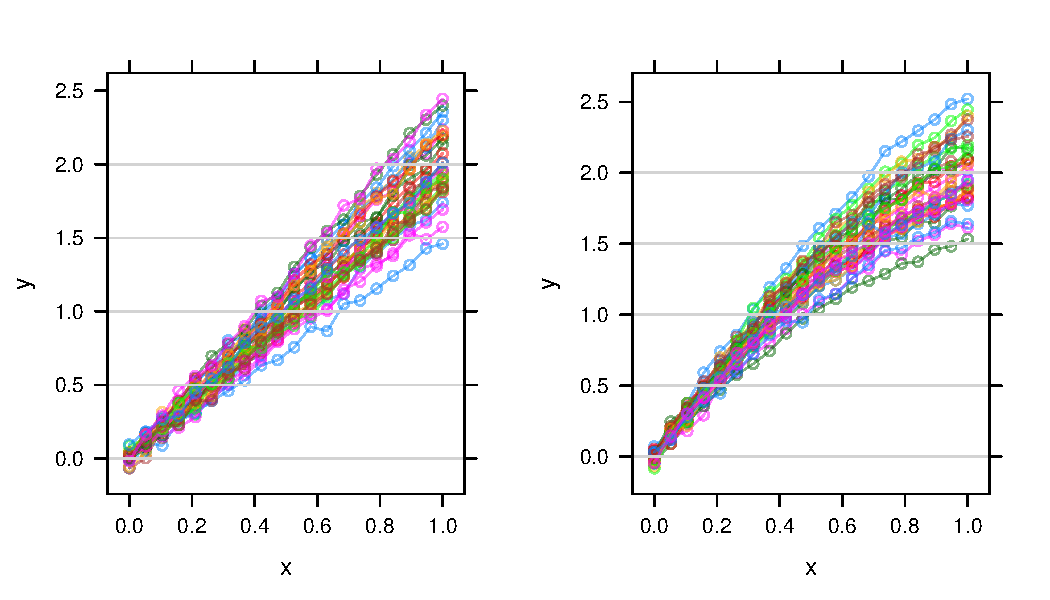
\includegraphics[width=\maxwidth]{figure/simdata-scatterplots} \caption[Scatterplots of simulated data]{Scatterplots of simulated data. \textit{Left}: Data from a balanced random intercept and slope model. \textit{Right}: Data from a balanced random intercept and slope model with a fixed quadratic term. The mean response is shown as a solid black curve and the dashed lines indicate the positions of the true unknowns $\left(x_0, \mc{Y}_0\right).$\label{fig:simdata-scatterplots}}
\end{figure}


\end{knitrout}


\begin{table}[!htb]
\centering
\caption[Coverage probability and length estimates for balanced random intercept and slope model]{Coverage probability and length estimates of calibration intervals corresponding to various values of $\mc{Y}_0$ in a balanced random intercept and slope model. The Monte Carlo sample size was $N = 1,000$ and the bootstrap sample size was $R = 999$. \label{tab:linear-results}}
\begin{tabular}{llcccccc}
  \toprule
            &  $\mathcal{Y}_0 =$ & 0    & 0.5  & 1    & 1.5  & 2    \\
  \hline
  Coverage  &  Wald                 & 0.95 & 0.94 & 0.93 & 0.94 & 0.93 \\
            &  Inversion            & 0.95 & 0.95 & 0.94 & 0.93 & 0.95 \\
            &  Percentile bootstrap & 0.95 & 0.94 & 0.93 & 0.93 & 0.94 \\
%             &  PB inversion (1)  & 0.94 & 0.94 & 0.95 & 0.95 & 0.95 \\
  					&  Adjusted inversion   & 0.96 & 0.94 & 0.94 & 0.94 & 0.96 \\
  \hline
  Length    &  Wald                 & 0.09 & 0.14 & 0.24 & 0.35 & 0.45 \\
            &  Inversion            & 0.09 & 0.14 & 0.24 & 0.34 & 0.45 \\
            &  Percentile bootstrap & 0.09 & 0.14 & 0.24 & 0.34 & 0.45 \\
%             &  PB inversion (1)  & 0.09 & 0.15 & 0.25 & 0.38 & 0.50 \\
						&  Adjusted inversion   & 0.09 & 0.14 & 0.24 & 0.36 & 0.47 \\
  \bottomrule
\end{tabular}
\end{table}

\begin{table}[!htb]
\centering
\caption[Coverage probability and length estimates for balanced a random intercept and slope model with quadratic term]{Coverage probability and length estimates of 95\% calibration intervals corresponding to various values of $\mc{Y}_0$ in a balanced random intercept and slope model containing a quadratic term. The Monte Carlo sample size was $N = 1,000$ and the bootstrap sample size was $R = 999$. \label{tab:quadratic-results}}
\begin{tabular}{llcccccc}
  \toprule
            &  $\mathcal{Y}_0 =$ & 0    & 0.5  & 1    & 1.5  & 2    \\
  \hline
  Coverage  &  Wald                 & 0.95 & 0.96 & 0.94 & 0.94 & 0.87 \\
            &  Inversion            & 0.96 & 0.95 & 0.94 & 0.93 & 0.93 \\
            &  Percentile bootstrap & 0.94 & 0.93 & 0.93 & 0.93 & 0.92 \\
%             &  PB inversion (1)  & 0.93 & 0.93 & 0.93 & 0.00 & 0.76 \\
						&  Adjusted inversion   & 0.94 & 0.94 & 0.94 & 0.93 & 0.92 \\
  \hline
  Length    &  Wald                 & 0.04 & 0.08 & 0.17 & 0.35 & 1.09 \\
            &  Inversion            & 0.04 & 0.08 & 0.16 & 0.38 & 1.36 \\
            &  Percentile bootstrap & 0.04 & 0.08 & 0.16 & 0.37 & 0.63 \\
%             &  PB inversion (1)  & 0.04 & 0.08 & 0.18 & 0.00 & 1.15 \\
						&  Adjusted inversion   & 0.04 & 0.08 & 0.17 & 0.37 & 1.37 \\
  \bottomrule
  \end{tabular}
\end{table}

% \begin{table}[!htb]
% \centering
% \caption[Coverage probability and length estimates for balanced a random intercept and slope model with quadratic term]{Coverage probability and length estimates of 95\% calibration intervals corresponding to various values of $\mc{Y}_0$ in a balanced random intercept and slope model containing a quadratic term. The Monte Carlo sample size was $N = 1,000$ and the bootstrap sample size was $R = 999$. \label{tab:quadratic-results}}
% \begin{tabular}{llcccccc}
%   \toprule
%             &  $\mathcal{Y}_0 =$ & 0    & 0.5  & 1    & 1.5  & 2    \\
%   \hline
%   Coverage  &  Wald                 & 0.95 & 0.96 & 0.94 & 0.94 & 0.87 \\
%             &  Inversion            & 0.96 & 0.95 & 0.94 & 0.93 & 0.93 \\
%             &  Percentile bootstrap & 0.94 & 0.93 & 0.93 & 0.00 & 0.92 \\
% %             &  PB inversion (1)  & 0.93 & 0.93 & 0.93 & 0.00 & 0.76 \\
%   					&  Adjusted inversion   & 0.94 & 0.94 & 0.94 & 0.00 & 0.92 \\
%   \hline
%   Length    &  Wald                 & 0.04 & 0.08 & 0.17 & 0.35 & 1.09 \\
%             &  Inversion            & 0.04 & 0.08 & 0.16 & 0.38 & 1.36 \\
%             &  Percentile bootstrap & 0.04 & 0.08 & 0.16 & 0.00 & 0.63 \\
% %             &  PB inversion (1)  & 0.04 & 0.08 & 0.18 & 0.00 & 1.15 \\
% 						&  Adjusted inversion   & 0.04 & 0.08 & 0.17 & 0.00 & 1.37 \\
%   \bottomrule
%   \end{tabular}
% \end{table}

As expected, all four procedures perform well for the balanced random intercept and slope model, with coverage estimates close to $0.95$ (see Table~\ref{tab:linear-results}). For the model with the quadratic term, the methods still performed well, however, the Wald-based interval performed much worse for $\mathcal{Y}_0 = 2$, with coverage probability well below $0.95$ (see Table~\ref{tab:quadratic-results}). A decrease in coverage was anticipated since we do not expect the sampling distribution of the inverse estimator, $\widehat{x}_0$, to be approximately normal (or even symmetric) in this portion of the curve. Surprisingly, the inversion interval seems to perform as well as the intervals based on the parametric bootstrap with respect to coverage. However, the interval based on the percentile bootstrap has the advantage of providing an estimate of the entire sampling distribution of $\widehat{x}_0$, rather than just a confidene interval, as well as good width. Also, the Wald-based and inversion intervals do not account for the uncertainty in the estimated variance components and rely on large-sample sizes, therefore, these intervals would not be expected to perform as well on smaller data sets. A more extensive simulation study allowing for different sample size configurations would be necessary to further substantiate these claims.

\section{Bladder volume example}
\label{sec:bladder-example}
In this section, we discuss an example involving a real dataset taken from \citet{brown_measurement_1993} where the author states:
\begin{quotation}
\noindent``A series of 23 women patients attending a urodynamic clinic were recruited for the study. After successful voiding of the bladder, sterile water was introduced in additions of 10, 15, and then 25 ml increments up to a final cumulative total of 175 ml. At each volume a measure of height ($\texttt{H}$) in mm and depth ($\texttt{D}$) in mm of largest ultrasound bladder images were taken. The product $\texttt{H} \times \texttt{D}$ was taken as a measure of liquid volume...''
\end{quotation}
The product of $\texttt{H}$ and $\texttt{D}$ is plotted against true volume in Figure~\ref{fig:bladder-scatter} for each of the 23 subjects. As can be seen from this plot, each subject has a slightly nonlinear trend and there are some missing observations (i.e., the data are unbalanced). 

\begin{knitrout}
\definecolor{shadecolor}{rgb}{0.969, 0.969, 0.969}\color{fgcolor}\begin{figure}[H]

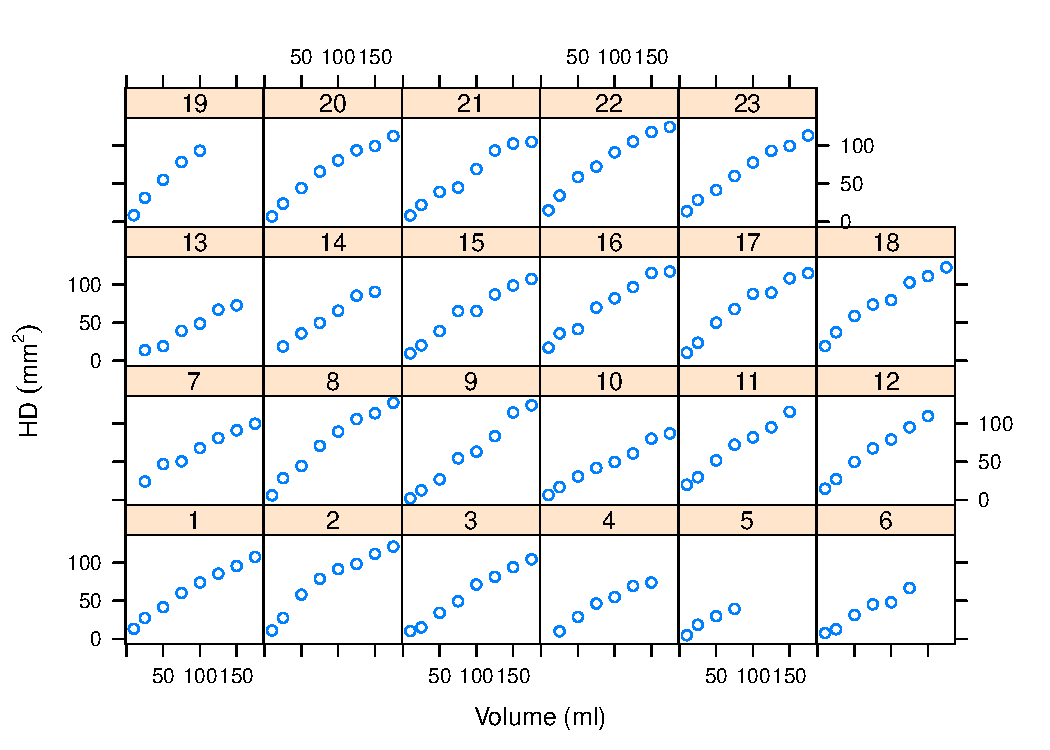
\includegraphics[width=\maxwidth]{figure/bladder-scatter} \caption[Scatterplot of the bladder volume data]{Scatterplot of the bladder volume data.\label{fig:bladder-scatter}}
\end{figure}


\end{knitrout}


Finding an appropriate random effects structure for the model can be difficult. An informal, but simple, approach is to fit the same model to the data for each subject and compare the estimated coefficients. To this end, we fit a simple quadratic model, $\mu(x) = \beta_0 + \beta_1 x + \beta_2 x^2$, to each of the 23 subjects measurements. Plots of the individual 95\% confidence intervals are displayed in Figure~\ref{fig:bladder-intervals}. We should point out that we used orthogonal polynomials to obtain each fit; this was done to remove the correlation between the estimated coefficients. Clearly, the intercept and slope parameters, $\beta_0$ and $\beta_1$, vary greatly between subjects, while $\beta_2$ remains relatively constant throughout. This suggests an \ac{LMM} with random effects for the intercept and linear terms. In particular, we used the following random coefficient model:
\begin{equation}
\label{eqn:bladder-lmm}
  \texttt{HD}_{ij} = \beta_0+\alpha_{0i} + \left(\beta_1+\alpha_{1i}\right)\texttt{volume}_{ij} + \beta_3\texttt{volume}_{ij}^2.
\end{equation}
Notice this is just the linear random trend model (Equation~\eqref{eqn:linear-random-trend}) with an additional quadratic term. Figure~\ref{fig:bladder-fit} shows the subject-specific fits based on model~\eqref{eqn:bladder-lmm}. Clearly, the model does a good job describing the data. Figure~\ref{fig:bladder-fit} also shows how each subject deviates from the overall fitted mean response $\wh{\mu}\left(x\right) = \wh{\beta}_0 + \wh{\beta}_1 x + \wh{\beta}_2 x^2$.

\begin{knitrout}
\definecolor{shadecolor}{rgb}{0.969, 0.969, 0.969}\color{fgcolor}\begin{figure}[H]

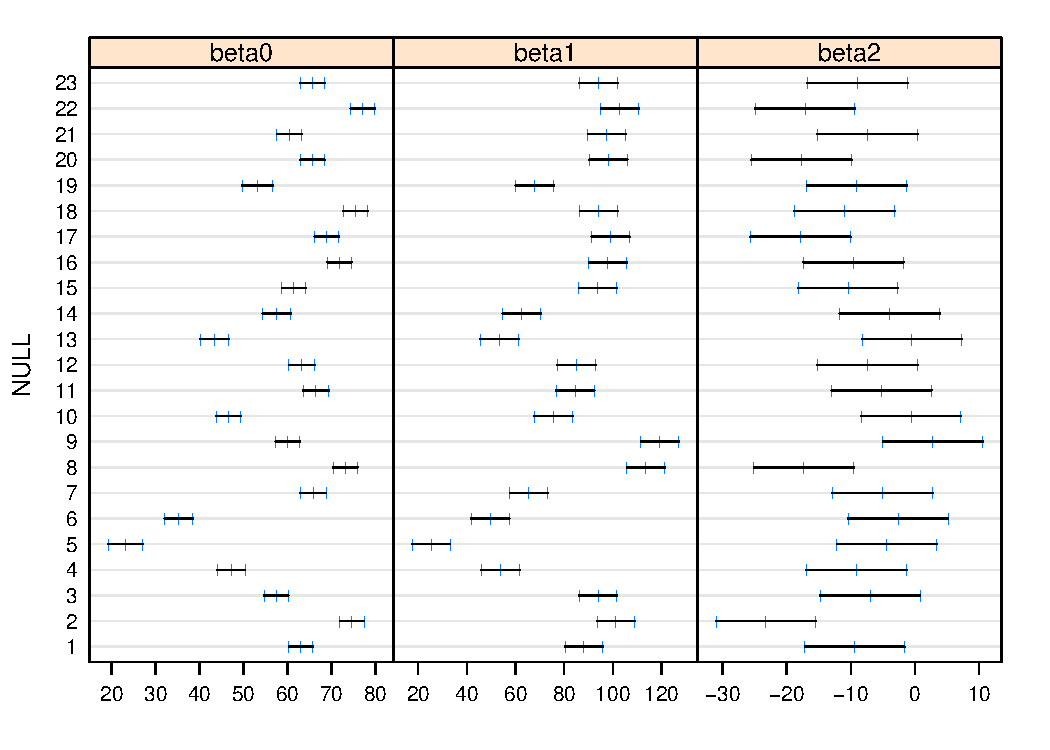
\includegraphics[width=\maxwidth]{figure/bladder-intervals} \caption[95\% confidence intervals for the bladder volume example]{95\% confidence intervals for regression coefficients from subject-specific fits to the bladder volume data. Note that we used orthogonal polynomials in order to remove the correlation between the estimated coefficients.\label{fig:bladder-intervals}}
\end{figure}


\end{knitrout}


\begin{knitrout}
\definecolor{shadecolor}{rgb}{0.969, 0.969, 0.969}\color{fgcolor}\begin{figure}[H]

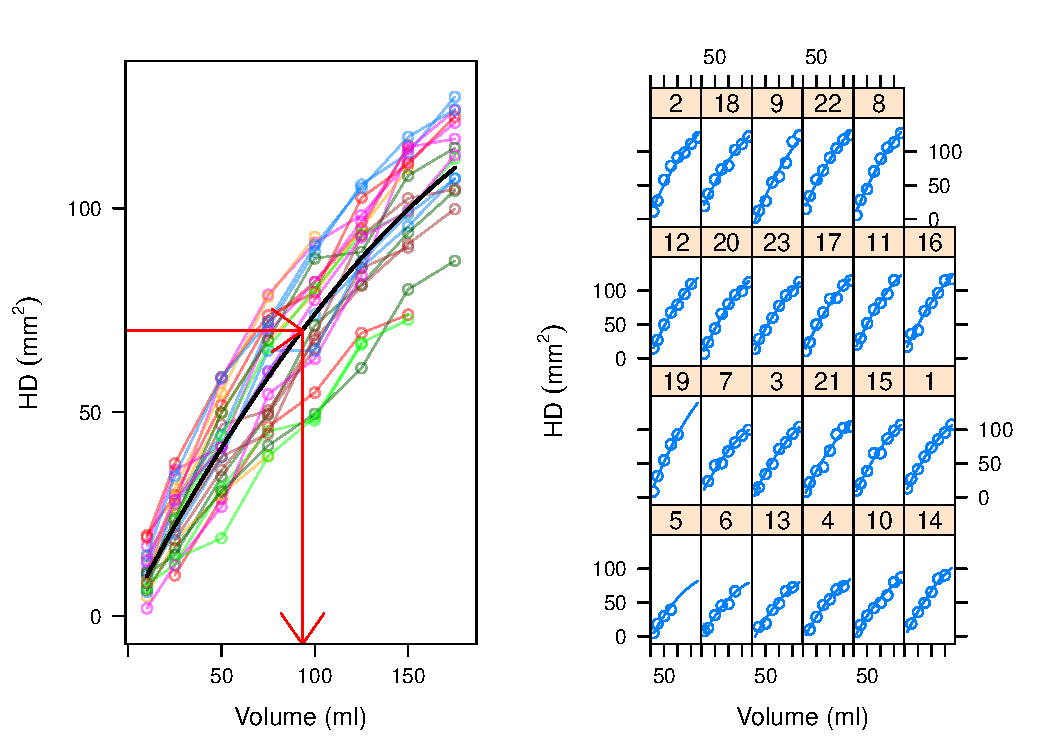
\includegraphics[width=\maxwidth]{figure/bladder-fit} \caption[Scatterplot of the bladder volume data with fitted mean response]{Scatterplot of the bladder volume data with fitted mean response. \textit{Left}: Scatterplot of the bladder volume data with fitted mean response (solid black curve). The horizontal red arrows indicate the positions of the unknown $\texttt{HD}_0 = 70 \text{ mm}^2$ and the point estimate $\wh{\texttt{volume}}_0$ obtained from inverting the fitted mean response. \textit{Right}: Fitted curves from a quadratic model fit to the bladder volume data. The model includes (uncorrelated) random effects for the intercept and linear term for each subject.\label{fig:bladder-fit}}
\end{figure}


\end{knitrout}


Suppose we obtain a new observation, $\texttt{HD}_0 = 70 \text{ mm}^2$, for which the true volume is unknown. To estimate the unknown volume, denoted $\texttt{volume}_0$, we proceed as discussed at the end of Section~\ref{sec:calibration-lmm-point}. In particular, we solve the equation 
\begin{equation*}
\wh{\mu}\left(\texttt{volume}_0\right) = \wh{\beta}_0 + \wh{\beta}_1\texttt{volume}_0 + \wh{\beta}_2\texttt{volume}_0^2 = 70 \text{ mm}^2
\end{equation*}
for $\texttt{volume}_0$ using the quadratic formula. The point estimate obtained is $\wh{\texttt{volume}}_0 = 93.4124$ ml (see Figure~\ref{fig:bladder-fit}). Since $\wh{\texttt{volume}}_0$ is not the \ac{ML} estimate, we cannot compute an approximate \ac{ML} interval as we could for the balanced random intercept example. However, the following snippet of \code{R} code shows how to use the well-known \pkg{car} package \citep{fox_r_2011} to compute the approximate standard error based on the first-order Taylor series estimate given in Equation~\eqref{eqn:cal-lmm-approx}. Note that our model has $\var\left\{\mc{Y}_0\right\} = \sigma_0^2 + x_0^2\sigma_1^2 + \sigma_\epsilon^2$ where $\sigma_0^2$ and $\sigma_1^2$ are the variances of the random intercept and linear terms, respectively. If the random effects were correlated, there would be an additional term $x_0\sigma_{01}$ where $\sigma_{01} = \cov\left\{\alpha_{0i}, \alpha_{1i}\right\}$. 

\begin{knitrout}
\definecolor{shadecolor}{rgb}{0.969, 0.969, 0.969}\color{fgcolor}\begin{kframe}
\begin{rexample}\label{bladder-wald}\hfill{}\begin{alltt}
\hlcom{## Obtain fitted model}
\hlstd{mod} \hlkwb{<-} \hlkwd{lme}\hlstd{(HD} \hlopt{~} \hlstd{volume} \hlopt{+} \hlkwd{I}\hlstd{(volume}\hlopt{^}\hlnum{2}\hlstd{),} \hlkwc{random} \hlstd{=} \hlkwd{pdDiag}\hlstd{(}\hlopt{~}\hlstd{volume),}
    \hlkwc{data} \hlstd{= Bladder)}
\hlstd{b} \hlkwb{<-} \hlkwd{as.numeric}\hlstd{(}\hlkwd{fixef}\hlstd{(mod))}  \hlcom{# vector of fixed effects}
\hlcom{## Set up variance-covariance matrix from Equation (5.7)}
\hlstd{var.y0} \hlkwb{<-} \hlkwd{getVarCov}\hlstd{(mod)[}\hlnum{1}\hlstd{,} \hlnum{1}\hlstd{]} \hlopt{+} \hlstd{x0.est}\hlopt{^}\hlnum{2} \hlopt{*} \hlkwd{getVarCov}\hlstd{(mod)[}\hlnum{2}\hlstd{,} \hlnum{2}\hlstd{]} \hlopt{+}
    \hlkwd{summary}\hlstd{(mod)}\hlopt{$}\hlstd{sigma}\hlopt{^}\hlnum{2}
\hlstd{covmat} \hlkwb{<-} \hlkwd{diag}\hlstd{(}\hlnum{4}\hlstd{)}
\hlstd{covmat[}\hlnum{1}\hlopt{:}\hlnum{3}\hlstd{,} \hlnum{1}\hlopt{:}\hlnum{3}\hlstd{]} \hlkwb{<-} \hlkwd{vcov}\hlstd{(mod)}
\hlstd{covmat[}\hlnum{4}\hlstd{,} \hlnum{4}\hlstd{]} \hlkwb{<-} \hlstd{var.y0}
\hlcom{## Call the deltaMethod() function from package car}
\hlstd{dm} \hlkwb{<-} \hlstd{car:::}\hlkwd{deltaMethod}\hlstd{(}\hlkwd{c}\hlstd{(}\hlkwc{b0} \hlstd{= b[}\hlnum{1}\hlstd{],} \hlkwc{b1} \hlstd{= b[}\hlnum{2}\hlstd{],} \hlkwc{b2} \hlstd{= b[}\hlnum{3}\hlstd{],} \hlkwc{y0} \hlstd{=} \hlnum{70}\hlstd{),}
    \hlkwc{g} \hlstd{=} \hlstr{"(-b1+sqrt(b1^2-4*b2*(b0-y0)))/(2*b2)"}\hlstd{,} \hlkwc{vcov.} \hlstd{= covmat)}
\hlkwd{rownames}\hlstd{(dm)} \hlkwb{<-} \hlstr{""}
\hlstd{dm}
\end{alltt}
\begin{verbatim}
##  Estimate    SE
##     93.41 19.63
\end{verbatim}
\end{rexample}\end{kframe}
\end{knitrout}





The resulting standard error is $19.63$ which yields an approximate (Wald-based) 95\% confidence interval for $\texttt{volume}_0$ of $(54.94, 131.89)$. For comparison, we computed the same interval assuming the data are cross-sectional, that is, by ignoring the grouped structure of the data and using the methods discussed in Section~\ref{sec:wald_int}. The resulting interval is $(56.43, 130.77$) which, as expected, is narrower than the one previously obtained.




Obtaining the inversion interval (Equation~\eqref{eqn:cal-lmm-inversion}) is less straightforward; we have to write our own prediction function in \code{R} that will also return the standard errors of the fitted values. Example~\ref{bladder-inversion} shows the minimal \code{R} code necessary to obtain $\wh{\mc{J}}_\mathrm{cal}(x)$ for the bladder volume example. The first line simply extracts the point estimate, $\wh{\texttt{volume}}_0$, obtained in Example~\ref{bladder-wald}. The next few lines of code define a new prediction function, \code{predFun}, that simply calls the built-in prediction function, but additionally returns the standard errors of the fitted values. The last block of code finds the roots to the equation $\mc{Q}^2 - z_{1-\alpha/2}^2 = 0$ where $\mc{Q}$ is the approximate pivot described in Section~\ref{sec:calibration-lmm-inversion}. The resulting interval, $(58.24, 137.05)$, is only slightly larger than the interval based on the delta method. Notice it is also not symmetric about the point estimate $\wh{\texttt{volume}}_0 = 93.41 \text{ ml}$ which, given the nonlinear trend and increasing variation in the data, is more realistic. 

\begin{knitrout}
\definecolor{shadecolor}{rgb}{0.969, 0.969, 0.969}\color{fgcolor}\begin{kframe}
\begin{rexample}\label{bladder-inversion}\hfill{}\begin{alltt}
\hlcom{## Extract point estimate from previous example}
\hlstd{x0.est} \hlkwb{<-} \hlstd{dm[[}\hlstr{"Estimate"}\hlstd{]]}
\hlcom{## Function to compute fitted values and their standard errors}
\hlstd{predFun} \hlkwb{<-} \hlkwa{function}\hlstd{(}\hlkwc{x}\hlstd{) \{}
    \hlstd{z} \hlkwb{<-} \hlkwd{list}\hlstd{(}\hlkwc{volume} \hlstd{= x)}
    \hlstd{fit} \hlkwb{<-} \hlkwd{predict}\hlstd{(mod,} \hlkwc{newdata} \hlstd{= z,} \hlkwc{level} \hlstd{=} \hlnum{0}\hlstd{)}
    \hlstd{se.fit} \hlkwb{<-} \hlkwd{sqrt}\hlstd{(}\hlkwd{diag}\hlstd{(}\hlkwd{cbind}\hlstd{(}\hlnum{1}\hlstd{,} \hlkwd{unlist}\hlstd{(z),} \hlkwd{unlist}\hlstd{(z)}\hlopt{^}\hlnum{2}\hlstd{)} \hlopt
        \hlstd{mod}\hlopt{$}\hlstd{varFix} \hlopt \hlkwd{t}\hlstd{(}\hlkwd{cbind}\hlstd{(}\hlnum{1}\hlstd{,} \hlkwd{unlist}\hlstd{(z),} \hlkwd{unlist}\hlstd{(z)}\hlopt{^}\hlnum{2}\hlstd{))))}
    \hlkwd{list}\hlstd{(}\hlkwc{fit} \hlstd{= fit,} \hlkwc{se.fit} \hlstd{= se.fit)}
\hlstd{\}}
\hlcom{## Invert approximate prediction bounds (numerically)}
\hlstd{invBounds} \hlkwb{<-} \hlkwa{function}\hlstd{(}\hlkwc{x}\hlstd{) \{}
    \hlstd{z} \hlkwb{<-} \hlkwd{list}\hlstd{(}\hlkwc{volume} \hlstd{= x)}
    \hlstd{(}\hlnum{70} \hlopt{-} \hlkwd{predFun}\hlstd{(x)}\hlopt{$}\hlstd{fit)}\hlopt{^}\hlnum{2}\hlopt{/}\hlstd{(var.y0} \hlopt{+} \hlkwd{predFun}\hlstd{(x)}\hlopt{$}\hlstd{se.fit}\hlopt{^}\hlnum{2}\hlstd{)} \hlopt{-}
        \hlkwd{qnorm}\hlstd{(}\hlnum{0.975}\hlstd{)}\hlopt{^}\hlnum{2}
\hlstd{\}}
\hlkwd{c}\hlstd{(}\hlkwd{uniroot}\hlstd{(invBounds,} \hlkwc{interval} \hlstd{=} \hlkwd{c}\hlstd{(}\hlnum{10}\hlstd{, x0.est),} \hlkwc{tol} \hlstd{=} \hlnum{1e-10}\hlstd{)}\hlopt{$}\hlstd{root,}
    \hlkwd{uniroot}\hlstd{(invBounds,} \hlkwc{interval} \hlstd{=} \hlkwd{c}\hlstd{(x0.est,} \hlnum{175}\hlstd{),} \hlkwc{tol} \hlstd{=} \hlnum{1e-10}\hlstd{)}\hlopt{$}\hlstd{root)}
\end{alltt}
\begin{verbatim}
## [1]  58.24 137.05
\end{verbatim}
\end{rexample}\end{kframe}
\end{knitrout}


In addition, we can also obtain the bootstrap adjusted inversion interval (Equation~\eqref{eqn:cal-lmm-inversion-boot}) described at the end of Section~\ref{sec:calibration-lmm-parboot}.
Figure~\ref{fig:bladder-parboot-hist1} shows a histogram of the $R = 9,999$ bootstrap replicates of $W$. As can be seen, the estimated sampling distribution of $W$ is reasonably normal. The necessary quantiles to compute $\wh{\mc{J}}_\mathrm{cal}^\boot(x)$ are $q_{0.025}^\boot = -2$ and $q_{0.975}^\boot = 1.98$ (compare these to the corresponding quantiles from a standard normal distribution; i.e., $\pm 1.96$)). Making the necessary adjustments to the code in Example~\ref{bladder-inversion} yields $\wh{\mc{J}}_\mathrm{cal}^\boot(x) = (57.94, 138.16)$, which is only slightly wider than the unadjusted inversion interval based on the normal approximation. In short, the normal approximation works quite well for these data.

\begin{knitrout}
\definecolor{shadecolor}{rgb}{0.969, 0.969, 0.969}\color{fgcolor}\begin{figure}[H]

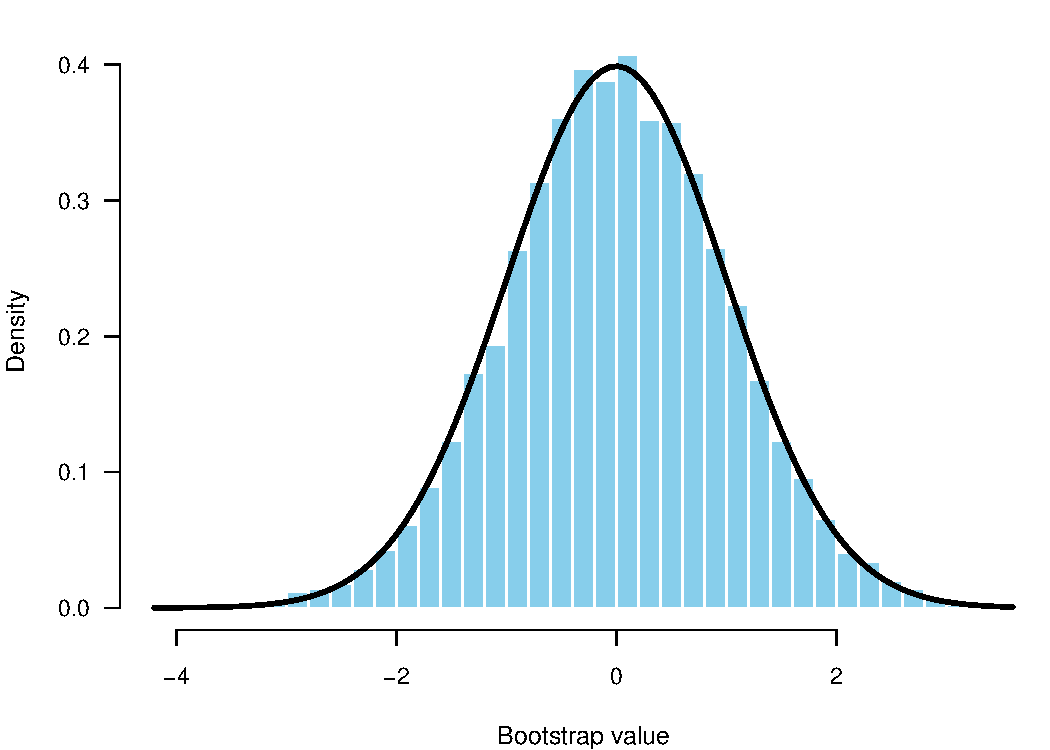
\includegraphics[width=\maxwidth]{figure/bladder-parboot-hist1} \caption[Bootstrap distribution of $\mc{Q}$ for the bladder volume example]{Bootstrap distribution of $W$ for the bladder volume example. A standard normal distribution (solid black curve) is shown for comparison.\label{fig:bladder-parboot-hist1}}
\end{figure}


\end{knitrout}


Finally, we compute the bootstrap distribution of $\wh{\texttt{volume}}_0$ directly using Algorithm~\ref{alg:parboot_cal}. Our results are based on a bootstrap simulation of size $R = 9,999$. Since we do not expect the sampling distribution of $\wh{\texttt{volume}}_0$ to be symmetric, we provide only a 95\% percentile bootstrap interval, that is, the interval obtained by taking the lower 2.5 and upper 97.5 percentiles of the bootstrap distribution. The resulting interval, $(58.37, 136.02)$, is quite close to the inversion interval previously obtained. A histogram of the $9,999$ bootstrap replicates of $\wh{\texttt{volume}}_0$ is given in Figure~\ref{fig:bladder-parboot-hist2}. As indicated by the normal Q-Q plot in Figure~\ref{fig:bladder-parboot-hist2}, the bootstrap distribution is positively skewed (the estimated skewness is $0.3011$), providing further support for the inversion and percentile intervals over the symmetric Wald-based interval obtained earlier using the delta method. 

\begin{knitrout}
\definecolor{shadecolor}{rgb}{0.969, 0.969, 0.969}\color{fgcolor}\begin{figure}[H]

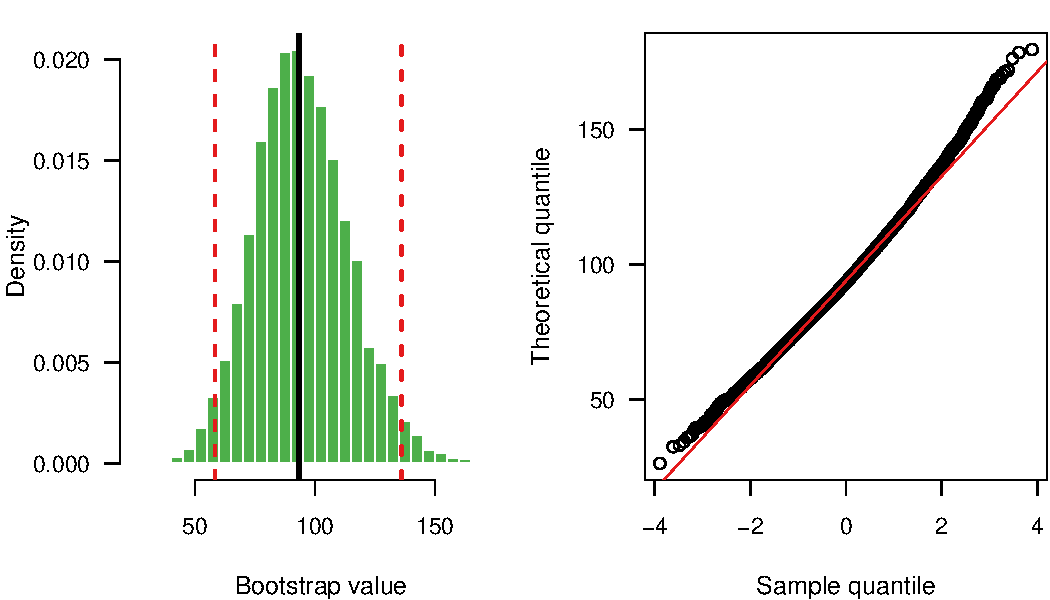
\includegraphics[width=\maxwidth]{figure/bladder-parboot-hist2} \caption[Bootstrap distribution of $\wh{\texttt{volume}}_0$ obtained using Algorithm~\ref{alg:parboot_cal}]{Bootstrap distribution of $\wh{\texttt{volume}}_0$ obtained using Algorithm~\ref{alg:parboot_cal}. \textit{Left}: Bootstrap distribution of $\wh{\texttt{volume}}_0$ obtained using Algorithm~\ref{alg:parboot_cal}. The solid black line indicates the original point estimate and the dotted red lines indicate the positions of the sample 2.5 and 97.5 quantiles of the bootstrap distribution. \textit{Right}: Normal Q-Q plot of the bootstrap replicates of $\wh{\texttt{volume}}_0$.\label{fig:bladder-parboot-hist2}}
\end{figure}


\end{knitrout}


\section{Discussion}
We have described a number of techniques for controlled calibration in a (linear) mixed model setting. The Wald-based interval is the simplest, but relies on the asymptotic normality of $\wh{x}_0$ along with a Taylor-series approximation of its variance. Perhaps the biggest drawback to using a Wald-based calibration interval is that it is always symmetric about $\wh{x}_0$. While this is appealing to many researchers, it is not very realistic in standard situations where, say, the data exhibit nonlinear behavior (possibly due to horizontal asymptotes) and nonconstant variance. The asymptotic normality of $\wh{x}_0$ may also be questioned when $\wh{x}_0$ is not the \ac{ML} estimate (as in the bladder volume example). This is akin to using the Wald-based method for nonlinear calibration problems (the software JMP does this). Nonetheless, the estimated sampling distribution of $\wh{x}_0$ displayed in Figures~\ref{fig:simdata-parboot-hist} and \ref{fig:bladder-parboot-hist2} using the parametric bootstrap are both reasonably normal. Thus, the Wald-based approach may still produce reliable inference when the distribution of $\wh{x}_0$ can be considered symmetric. Although more difficult to obtain, the inversion and parametric bootstrap  intervals are presumably superior to the Wald-based interval.

All the methods we have proposed rely on certain assumptions, for example, normality and large sample size. These assumptions may or may not hold in practice. If the random effects and errors are not normally distributed, then it is possible to fit a non-Gaussian mixed model \citep[p. 8]{jiang_linear_2007}. In this situation, we can still calculate a calibration interval by inverting a corresponding distribution-free prediction interval with asymptotic coverage probability $1-\alpha$. As we have shown in Section~\ref{sec:calibration-lmm-distfree}, this is rather simple to do for standard LMMs. If, on the other hand, the data are not normal and the sample size is rather small, then there is not much we can do with the methods discussed in this chapter. 

Future work on data like these might combine the nonparametric method of calibration proposed in Chapter~\ref{chap:nonparametric} with the application to grouped data discussed in this chapter. In particular, we would recognize the grouped structure of the data but allow each specimen to have its own (nonlinear) trend by introducing subject-specific spline terms which may or may not have corresponding random effects. This may seem far-fetched at first, but remember that the specific approach we took for nonparametric calibration is already based on an \ac{LMM} \eqref{eqn:spline-model-lme}. This is an obvious, and likely promising, area of future research, and we discuss it, along with some other ideas, in the conclusion to this dissertation.



%% Conclusion ------------------------------------------------------------------

% !Rnw root = Master.Rnw

\chapter{Conclusions and Suggestions for Further Research}
\label{chp:conclusion}
Statistical calibration is an important application of regression in many areas of science, for example: bioassays, chemometrics, and calibrating laboratory equipment. For many of these applications, the data are inherently nonlinear with no known parametric form, or sometimes the data are collected in such a way that the observations can not be considered as independent. It is necessary, then, to have simple and general methods available for calibration in these situations. This has been the main goal of our research.

\section{Conclusions}
We discussed (controlled) semiparametric calibration in Chapter~\ref{chap:nonparametric}. We provided a frequentist approach to obtaining calibration intervals that involved inverting bias-corrected prediction intervals based on the simple LMM-based smoother described in \citet{ruppert_semiparametric_2003}. The coverage probability and length of these intervals were investigated using a small Monte Carlo experiment. This experiment showed that these intervals do in fact obtain coverage probability close to the nominal $1-\alpha$ level without sacrificing length. The experiment also highlighted that correcting for bias is more serious for calibration with respect to a mean response (i.e., regulation). A simple Bayesian analog was also proposed that has the benefit of providing the entire posterior distribution of $x_0$. We illustrated these methods using real data analysis examples.

In Chapter~\ref{chp:cal-dependent}, we extended the usual methods of (controlled) calibration (i.e., point estimation and obtaining Wald-based/inversion intervals) for grouped data using the LMM. We also proposed a parametric bootstrap algorithm for controlled calibration in the LMM. This algorithm can be used to obtain confidence intervals for the unknown $x_0$ directly from the estimated sampling distribution of the point estimator $\widehat{x}_0$, or by improving the inversion interval by removing the normality constraint on the approximate predictive pivot $\mathcal{W}$. These strategies were illustrated using real data analysis examples. We also briefly described how to use a distribution-free prediction interval to obtain a distribution-free inversion interval for the unknown $x_0$ in closed form for the random intercept model.

Calibration will always remain an important topic in statistics. We list here some possible topics for future research based on extending the ideas in Chapters~\ref{chap:nonparametric} and \ref{chp:cal-dependent}:
\begin{itemize}
  \item Semiparametric calibration with constraints;
  \item Prior selection for $x_0$ in semiparametric calibration;
  \item Bootstrap for (controlled) semiparametric calibration;
  \item Calibration in NLMMs;
  \item Semiparametric calibration with random coefficients.
\end{itemize}
For the most part, these topics were discussed in the conclusions to Chapters~\ref{chap:nonparametric} and \ref{chp:cal-dependent}.


%% Appendix --------------------------------------------------------------------

% !Rnw root = Master.Rnw

\appendix  	% Appendix begins here

\chapter{Proofs}
\label{app:proofs}
In this appendix, we provide the "extra steps" for deriving some of the mathematical results presented in this dissertation.

\section{Conditional posterior of \texorpdfstring{$\left(\boldsymbol{\beta}, \boldsymbol{\alpha}\right)$}{polynomial and spline coefficients}}
\label{sec:conditional-theta}
Note that the kernel of a multivariate normal distribution with mean vector $\boldsymbol{\mu}$ and variance-covariance matrix $\boldsymbol{\Sigma}$ is 
\begin{equation*}
  K\left(\boldsymbol{x}; \boldsymbol{\mu}, \boldsymbol{\Sigma}\right) \propto \exp\left\{-\frac{1}{2}\left(\boldsymbol{x}-\boldsymbol{\mu}\right)'\boldsymbol{\Sigma}^{-1}\left(\boldsymbol{x}-\boldsymbol{\mu}\right)\right\}.
\end{equation*}
Furthermore, let $\boldsymbol{x}$ and $\boldsymbol{\theta}$ be $n \times 1$ vectors, and  $\boldsymbol{A}$ be an invertible $n \times n$ symmetric matrix. We can \href{http://en.wikipedia.org/wiki/Completing_the_square}{complete the square for the quadratic form} $\boldsymbol{x}'\boldsymbol{A}\boldsymbol{x} - \boldsymbol{\theta}'\boldsymbol{x}$ by writing
\begin{equation*}
  \boldsymbol{x}'\boldsymbol{A}\boldsymbol{x} - \boldsymbol{\theta}'\boldsymbol{x} = \left(\boldsymbol{x}-\boldsymbol{\mu}\right)'\boldsymbol{A}^{-1}\left(\boldsymbol{x}-\boldsymbol{\mu}\right) + C,
\end{equation*}
where 
\begin{equation*}
  \boldsymbol{\mu} = \frac{1}{2}\boldsymbol{A}^{-1}\boldsymbol{\theta} \quad \text{and} \quad C = -\frac{1}{4}\boldsymbol{\theta}'\boldsymbol{A}^{-1}\boldsymbol{\theta}.
\end{equation*}

Let the vectors $\boldsymbol{x}_0$ and $\boldsymbol{z}_0$ have the same form as the $i$-th rows of $\boldsymbol{X}$ and $\boldsymbol{Z}$ in Equation~\eqref{eqn:spline-model-lme}, respectively, but with $x_i$ replaced with $x_0$. Ignoring the constant of proportionality, the conditional posterior of $\left(\boldsymbol{\beta}, \boldsymbol{\alpha}\right)$ is
\begin{align*}
  \pi\left(\boldsymbol{\beta}, \boldsymbol{\alpha}|\boldsymbol{y}, y_0, \sigma_\epsilon^2, \sigma_\alpha^2, x0\right) &\propto \pi\left(\boldsymbol{y}|\boldsymbol{\beta}, \boldsymbol{\alpha}, \sigma_\epsilon^2, \sigma_\alpha^2, x_0\right) \pi\left(y_0|\boldsymbol{\beta}, \boldsymbol{\alpha}, \sigma_\epsilon^2, \sigma_\alpha^2, x_0\right) \pi\left(\boldsymbol{\beta}\right) \pi\left(\boldsymbol{\alpha}|\sigma_\alpha^2\right) \\
  &\propto \exp\left\{-\frac{1}{2\sigma_\epsilon^2}||\boldsymbol{y} - \boldsymbol{X}\boldsymbol{\beta} - \boldsymbol{Z}\boldsymbol{\alpha}||^2 - \frac{1}{2\sigma_\alpha^2}||\boldsymbol{\alpha}||^2 - \frac{1}{2\sigma_\epsilon^2}\left[y_0-\mu(x_0)\right]^2\right\} \\
  &= \exp\left\{-\frac{1}{2\sigma_\epsilon^2}\left(||\boldsymbol{y} - \boldsymbol{X}\boldsymbol{\beta} - \boldsymbol{Z}\boldsymbol{\alpha}||^2 + \left[y_0-\mu(x_0)\right]^2 + \frac{\sigma_\epsilon^2}{\sigma_\alpha^2}||\boldsymbol{\alpha}||^2\right)\right\} \\
  &= \exp\left\{-\frac{1}{2\sigma_\epsilon^2}\left(||\boldsymbol{y} - \boldsymbol{X}\boldsymbol{\beta} - \boldsymbol{Z}\boldsymbol{\alpha}||^2 + \left(y_0-\boldsymbol{x}_0'\boldsymbol{\beta} - \boldsymbol{z}_0'\boldsymbol{\alpha}\right)^2 + \frac{\sigma_\epsilon^2}{\sigma_\alpha^2}||\boldsymbol{\alpha}||^2\right)\right\} \\
  &= \exp\left\{-\frac{1}{2\sigma_\epsilon^2}\left(||\boldsymbol{y}_0 - \boldsymbol{X}_0\boldsymbol{\beta} - \boldsymbol{Z}_0\boldsymbol{\alpha}||^2 + \frac{\sigma_\epsilon^2}{\sigma_\alpha^2}||\boldsymbol{\alpha}||^2\right)\right\},
\end{align*}
where 
\begin{equation*}
  \boldsymbol{y}_0 = \begin{bmatrix} \boldsymbol{y} \\ y_0 \end{bmatrix}, \quad
  \boldsymbol{X}_0 = \begin{bmatrix} \boldsymbol{X} \\ \boldsymbol{x}_0' \end{bmatrix}, \quad
  \boldsymbol{Z}_0 = \begin{bmatrix} \boldsymbol{Z} \\ \boldsymbol{z}_0' \end{bmatrix}
\end{equation*}
are augmented data vectors and matrices. To show that the conditional posterior of $\boldsymbol{\theta} = \left(\boldsymbol{\beta}', \boldsymbol{\alpha}'\right)'$ is normal, note that
\begin{align*}
  &\exp\left\{-\frac{1}{2\sigma_\epsilon^2}\left(||\boldsymbol{y}_0 - \boldsymbol{X}_0\boldsymbol{\beta} - \boldsymbol{Z}_0\boldsymbol{\alpha}||^2 + \frac{\sigma_\epsilon^2}{\sigma_\alpha^2}||\boldsymbol{\alpha}||^2\right)\right\} \\
  &= \exp\left\{-\frac{1}{2\sigma_\epsilon^2}||\boldsymbol{y}_0^* - \boldsymbol{X}_0^*\boldsymbol{\beta} - \boldsymbol{Z}_0^*\boldsymbol{\alpha}||^2\right\} \\
  &= \exp\left\{-\frac{1}{2\sigma_\epsilon^2}||\boldsymbol{y}_0^* - \boldsymbol{\Omega}_0^*\boldsymbol{\theta}||^2\right\},
\end{align*}
where, similar to before,
\begin{equation*}
  \boldsymbol{y}_0^* = \begin{bmatrix} \boldsymbol{y}_0 \\ \boldsymbol{0} \end{bmatrix}, \quad
  \boldsymbol{X}_0^* = \begin{bmatrix} \boldsymbol{X}_0 \\ \boldsymbol{0} \end{bmatrix}, \quad
  \boldsymbol{Z}_0^* = \begin{bmatrix} \boldsymbol{Z}_0 \\ \left(\sigma_\epsilon^2/\sigma_\alpha^2\right)\boldsymbol{I} \end{bmatrix}
\end{equation*}
are augmented data vectors and matrices and $\boldsymbol{\Omega}_0^* = \left(\boldsymbol{X}_0^*; \boldsymbol{Z}_0^*\right)$. Now, using basic matrix multiplication,
\begin{align*}
  \exp\left\{-\frac{1}{2\sigma_\epsilon^2}||{\boldsymbol{y}_0^*}' - \boldsymbol{\Omega}_0^*\boldsymbol{\theta}||^2\right\}
  &= \exp\left\{-\frac{1}{2\sigma_\epsilon^2}\left({\boldsymbol{y}_0^*}'\boldsymbol{y}_0^* - 2{\boldsymbol{y}_0^*}'\boldsymbol{\Omega}_0^*\boldsymbol{\theta} + \boldsymbol{\theta}'{\boldsymbol{\Omega}_0^*}'\boldsymbol{\Omega}_0^*\boldsymbol{\theta}\right)\right\} \\
  &\propto \exp\left\{-\frac{1}{2\sigma_\epsilon^2}\left(\boldsymbol{\theta}'{\boldsymbol{\Omega}_0^*}'\boldsymbol{\Omega}_0^*\boldsymbol{\theta} - 2{\boldsymbol{y}_0^*}'\boldsymbol{\Omega}_0^*\boldsymbol{\theta}\right)\right\}.
\end{align*}
Upon completing the square, we get
\begin{equation*}
  \exp\left\{-\frac{1}{2\sigma_\epsilon^2}\left(\boldsymbol{\theta}'{\boldsymbol{\Omega}_0^*}'\boldsymbol{\Omega}_0^*\boldsymbol{\theta} - 2{\boldsymbol{y}_0^*}'\boldsymbol{\Omega}_0^*\boldsymbol{\theta}\right)\right\} = \exp\left\{-\frac{1}{2}\left(\boldsymbol{\theta}-\boldsymbol{\mu}_{\boldsymbol{\theta}}\right)'\boldsymbol{\Sigma}_{\boldsymbol{\theta}}^{-1}\left(\boldsymbol{\theta}-\boldsymbol{\mu}_{\boldsymbol{\theta}}\right)\right\},
\end{equation*}
where
\begin{equation*}
  \boldsymbol{\mu}_{\boldsymbol{\theta}} = \left({\boldsymbol{\Omega}_0^*}'\boldsymbol{\Omega}_0^*\right)^{-1}{\boldsymbol{\Omega}_0^*}'\boldsymbol{y}_0^* = \left({\boldsymbol{\Omega}_0}'\boldsymbol{\Omega}_0 + \frac{\sigma_\epsilon^2}{\sigma_\alpha^2}\boldsymbol{D}\right)^{-1}{\boldsymbol{\Omega}_0}'\boldsymbol{y}_0, \quad \boldsymbol{D} = \textbf{diag}\left\{\boldsymbol{0}_{p \times p}, \boldsymbol{I}_{q \times q}\right\},
\end{equation*}
and
\begin{equation*}
  \boldsymbol{\Sigma}_{\boldsymbol{\theta}} = \sigma_\epsilon^2\left({\boldsymbol{\Omega}_0^*}'\boldsymbol{\Omega}_0^*\right)^{-1} = \sigma_\epsilon^2\left({\boldsymbol{\Omega}_0}'\boldsymbol{\Omega}_0\right)^{-1}.
\end{equation*}
Thus, the conditional posterior of the coefficients $\boldsymbol{\theta}$ is multivariate normal with mean vector $\boldsymbol{\mu}_{\boldsymbol{\theta}}$ and variance-covariance matrix $\boldsymbol{\Sigma}_{\boldsymbol{\theta}}$.

\section{Conditional posteriors of \texorpdfstring{$\sigma_\epsilon^2$ and $\sigma_\alpha^2$}{variance components}}
\label{sec:conditional-variances}
Note that since $\sigma_\epsilon^2 \sim \mathcal{IG}\left(a, b\right)$, then 
\begin{equation*}
  \pi(\sigma_\epsilon^2) = \frac{b^a}{\Gamma(a)}\left(\sigma_\epsilon^2\right)^{-(a+1)}\exp\left\{-\frac{b}{\sigma_\epsilon^2}\right\}.
\end{equation*}
Now, ignoring the constant of proportionality, the conditional posterior of $\sigma_\epsilon^2$ is
\begin{align*}
  \pi(\sigma_\epsilon^2|\boldsymbol{y}, y_0, \boldsymbol{\beta}, &\boldsymbol{\alpha}, \sigma_\alpha^2, x_0) \propto \pi(\boldsymbol{y}|\boldsymbol{\beta}, \boldsymbol{\alpha}, \sigma_\epsilon^2)\pi(y_0|\boldsymbol{\beta}, \boldsymbol{\alpha}, \sigma_\epsilon^2, x_0)\pi(\sigma_\epsilon^2) \\
  &\propto \left(\sigma_\epsilon^2\right)^{-(a+1)}\exp\left\{-\frac{||\boldsymbol{y} - \boldsymbol{X}\boldsymbol{\beta} - \boldsymbol{Z}\boldsymbol{\alpha}||^2}{2\sigma_\epsilon^2} - \frac{\left(y_0 - \boldsymbol{x}_0\boldsymbol{\beta} - \boldsymbol{z}_0\boldsymbol{\alpha}\right)^2}{2\sigma_\epsilon^2} - \frac{b}{\sigma_\epsilon^2}\right\} \\
  &= \left(\sigma_\epsilon^2\right)^{-(a+1)}\exp\left\{\frac{\left(\frac{1}{2}||\boldsymbol{y}_0 - \boldsymbol{X}_0\boldsymbol{\beta} - \boldsymbol{Z}_0\boldsymbol{\alpha}||^2 + b\right)}{\sigma_\epsilon^2}\right\},
\end{align*}
which is proportional to the density function of a $\mathcal{IG}\left(a, \frac{1}{2}||\boldsymbol{y}_0 - \boldsymbol{X}_0\boldsymbol{\beta} - \boldsymbol{Z}_0\boldsymbol{\alpha}||^2 + b\right)$ distribution. The proof for the conditional posterior $\pi(\sigma_\alpha^2|\boldsymbol{y}, y_0, \boldsymbol{\beta}, \boldsymbol{\alpha}, \sigma_\epsilon^2, x_0)$ follows in an analogous manner.

\section{LMM log-likelihood}
\label{eqn:lmm-log-likelihood}
For the LMM (Equation~\eqref{eqn:lmm-matrix}), we have that
\begin{equation*}
  \boldsymbol{\mathcal{Y}} \sim \mathcal{N}\left(\boldsymbol{X}\boldsymbol{\beta}, \boldsymbol{V}\right),
\end{equation*}
hence, the density function is
\begin{equation*}
  f(\boldsymbol{y}) = \left(2\pi\right)^{-N/2}\left|\boldsymbol{V}\right|^{-1/2}\exp\left\{-\frac{1}{2}\left(\boldsymbol{\mathcal{Y}} - \boldsymbol{X}\boldsymbol{\beta}\right)'\boldsymbol{V}^{-1}\left(\boldsymbol{\mathcal{Y}} - \boldsymbol{X}\boldsymbol{\beta}\right)\right\}.
\end{equation*}
Taking the logarithm of $f(\boldsymbol{y})$ gives the log-likelihood 
\begin{equation*}
  \ell = -\frac{N}{2}\log(2\pi) - \frac{1}{2}\log\left(\left|\boldsymbol{V}\right|\right) - \frac{1}{2}\left(\boldsymbol{\mathcal{Y}} - \boldsymbol{X}\boldsymbol{\beta}\right)'\boldsymbol{V}^{-1}\left(\boldsymbol{\mathcal{Y}} - \boldsymbol{X}\boldsymbol{\beta}\right).
\end{equation*}
Let $\boldsymbol{V}$ have the block diagonal form $\boldsymbol{V} = \sigma_\epsilon^2\Big\{_{\text{diag}} \boldsymbol{I}_{n_i} + \boldsymbol{Z}_i\boldsymbol{G}^*\boldsymbol{Z}_i' \Big\}_{i = 1}^m$. Since the determinant of a block diagonal matrix is just the product of the determinant of the block diagonals, then
\begin{align*}
  \log\left(\left|\boldsymbol{V}\right|\right) &= \log\left\{\prod_{i=1}^m\left|\sigma_\epsilon^2\left(\boldsymbol{I}_{n_i} + \boldsymbol{Z}_i\boldsymbol{G}^*\boldsymbol{Z}_i'\right)\right|\right\} \\
  &= \log\left\{\prod_{i=1}^m\left(\sigma_\epsilon^2\right)^{n_i}\left|\boldsymbol{I}_{n_i} + \boldsymbol{Z}_i\boldsymbol{G}^*\boldsymbol{Z}_i'\right|\right\} \\
  &= \sum_{i=1}^m n_i \log\left(\sigma_\epsilon^2\right) + \sum_{i=1}^m\log\left(\left|\boldsymbol{I}_{n_i} + \boldsymbol{Z}_i\boldsymbol{G}^*\boldsymbol{Z}_i'\right|\right) \\
  &= N\log\left(\sigma_\epsilon^2\right) + \sum_{i=1}^m\log\left(\left|\boldsymbol{I}_{n_i} + \boldsymbol{Z}_i\boldsymbol{G}^*\boldsymbol{Z}_i'\right|\right).
\end{align*}
Similarly, since the inverse of a block diagonal matrix is another block diagonal matrix, composed of the inverse of each block, it follows that
\begin{equation*}
  \left(\boldsymbol{\mathcal{Y}} - \boldsymbol{X}\boldsymbol{\beta}\right)'\boldsymbol{V}^{-1}\left(\boldsymbol{\mathcal{Y}} - \boldsymbol{X}\boldsymbol{\beta}\right) = \sum_{i=1}^m\left(\boldsymbol{\mathcal{Y}}_i - \boldsymbol{X}_i\boldsymbol{\beta}\right)'\boldsymbol{V}_i^{-1}\left(\boldsymbol{\mathcal{Y}}_i - \boldsymbol{X}_i\boldsymbol{\beta}\right),
\end{equation*}
where $\boldsymbol{V}_i = \sigma_\epsilon^2\left(\boldsymbol{I}_{n_i} + \boldsymbol{Z}_i\boldsymbol{G}^*\boldsymbol{Z}_i'\right)$. Therefore, the log-likelihood becomes
\begin{align*}
    \ell &= -\frac{N}{2}\log(2\pi) - \frac{1}{2}\log\left(\left|\boldsymbol{V}\right|\right) - \frac{1}{2}\left(\boldsymbol{\mathcal{Y}} - \boldsymbol{X}\boldsymbol{\beta}\right)'\boldsymbol{V}^{-1}\left(\boldsymbol{\mathcal{Y}} - \boldsymbol{X}\boldsymbol{\beta}\right) \\
    &= -\frac{N}{2}\log(2\pi) - \frac{N}{2}\log(\sigma_\epsilon^2) - \frac{1}{2}\sum_{i=1}^m\log\left(\left|\boldsymbol{I}_{n_i} + \boldsymbol{Z}_i\boldsymbol{G}^*\boldsymbol{Z}_i'\right|\right) \newln - \frac{1}{2\sigma_\epsilon^2}\sum_{i=1}^m\left(\boldsymbol{\mathcal{Y}}_i - \boldsymbol{X}_i\boldsymbol{\beta}\right)'\left(\boldsymbol{I}_{n_i} + \boldsymbol{Z}_i\boldsymbol{G}^*\boldsymbol{Z}_i'\right)^{-1}\left(\boldsymbol{\mathcal{Y}}_i - \boldsymbol{X}_i\boldsymbol{\beta}\right).
\end{align*}

\chapter{The \code{R} Package \pkg{investr}}
\label{app:investr}
In this appendix, we describe the \pkg{investr} package for the \code{R} statistical software. The name \pkg{investr} stands for \underline{inv}erse \underline{est}imation in \underline{R}. It is currently listed on CRAN at \url{http://cran.r-project.org/web/packages/investr/index.html}. The source code for additional functions (e.g., \code{pspline}) can be obtained from the GitHub development site at \url{https://github.com/w108bmg/Research/tree/master/Rcode}. To install the package, simply open an \code{R} terminal and type:

\begin{knitrout}
\definecolor{shadecolor}{rgb}{0.969, 0.969, 0.969}\color{fgcolor}\begin{kframe}
\begin{alltt}
\hlkwd{install.packages}\hlstd{(}\hlstr{"investr"}\hlstd{,} \hlkwc{dependencies} \hlstd{=} \hlnum{TRUE}\hlstd{)}  \hlcom{# install package}
\hlkwd{library}\hlstd{(investr)}  \hlcom{# load package}
\end{alltt}
\end{kframe}
\end{knitrout}

\noindent Once the package is loaded, we have access to all of its functions, datasets, and examples. The three main functions are described in Table~\ref{tab:investr}.
\begin{table}[H]
\label{tab:investr}
\begin{center}
\begin{tabular}{lp{10cm}}
  \toprule
  \textbf{Function} & \textbf{Description} \\
  \midrule
  \code{calibrate} & For a vector of $m$ response values with unknown predictor value $x_0$, computes the classical estimate (i.e., ML estimate) $\widehat{x}_0$ and a corresponding Wald or inversion interval for the simple linear calibration problem. \\
  \code{invest}    & For a vector of $m$ response values with unknown predictor value $x_0$, computes the classical estimate $\widehat{x}_0$ and a corresponding Wald or inversion interval for polynomial and nonlinear calibration problems. \\
  \code{plotFit}   & For plotting fitted regression models with or without confidence/prediction bands. \\
  \bottomrule
\end{tabular}
\end{center}
\caption[Functions from the \pkg{investr} package]{Main functions from the \pkg{investr} package.}
\end{table}

\section{The \code{plotFit} function}
The \code{plotFit} function is a general purpose function that is also useful outside of statistical calibration problems. Its sole purpose is to plot fitted models for \code{R} objects of class \code{lm} or class \code{nls} with the option of adding a confidence and/or prediction band. For example, the following snippet of \code{R} code fits a simple linear regression model to the $\code{crystal}$ data frame and plots the data along with the fitted regression line and (pointwise) $95\%$ confidence band. Of course, we can change the default $95\%$ confidence level by specifying, for example, $\code{level=0.9}$. Additionally, we can also specify an adjustment for simultaneous inference such as \textit{Scheff\'{e}}, \textit{Bonferroni}, or \textit{Working-Hotelling}. The second call to \code{plotFit} in the code below illustrates the use of both of these options.

\begin{knitrout}
\definecolor{shadecolor}{rgb}{0.969, 0.969, 0.969}\color{fgcolor}\begin{kframe}
\begin{alltt}
\hlkwd{par}\hlstd{(}\hlkwc{mfrow} \hlstd{=} \hlkwd{c}\hlstd{(}\hlnum{1}\hlstd{,} \hlnum{2}\hlstd{),} \hlkwc{cex.main} \hlstd{=} \hlnum{0.8}\hlstd{)}  \hlcom{# side-by-side plots}
\hlstd{crystal.lm} \hlkwb{<-} \hlkwd{lm}\hlstd{(weight} \hlopt{~} \hlstd{time,} \hlkwc{data} \hlstd{= crystal)}  \hlcom{# fit model}
\hlkwd{plotFit}\hlstd{(crystal.lm,} \hlkwc{interval} \hlstd{=} \hlstr{"confidence"}\hlstd{,} \hlkwc{shade} \hlstd{= T,}
    \hlkwc{col.conf} \hlstd{=} \hlstr{"skyblue"}\hlstd{,} \hlkwc{main} \hlstd{=} \hlstr{"95% pointwise confidence band"}\hlstd{)}
\hlkwd{plotFit}\hlstd{(crystal.lm,} \hlkwc{interval} \hlstd{=} \hlstr{"confidence"}\hlstd{,} \hlkwc{shade} \hlstd{= T,}
    \hlkwc{col.conf} \hlstd{=} \hlstr{"skyblue"}\hlstd{,} \hlkwc{level} \hlstd{=} \hlnum{0.9}\hlstd{,} \hlkwc{adjust} \hlstd{=} \hlstr{"W-H"}\hlstd{,}
    \hlkwc{main} \hlstd{=} \hlstr{"90% Working-Hotelling band"}\hlstd{)}
\end{alltt}
\end{kframe}
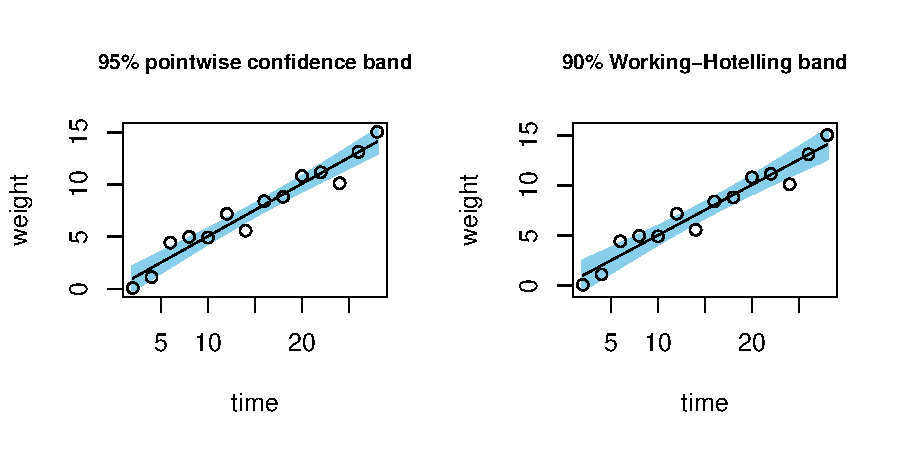
\includegraphics[width=\maxwidth]{figure/example-crystal-plotFit} 

\end{knitrout}


\noindent More elaborate models can also be plotted in the same way. For example, the following snippet of code fits a simple linear, quadratic, cubic, and natural cubic spline model to the well-known \code{cars} data frame and then plots the corresponding fits with both confidence and prediction bands at the 95\% level.

\begin{knitrout}
\definecolor{shadecolor}{rgb}{0.969, 0.969, 0.969}\color{fgcolor}\begin{kframe}
\begin{alltt}
\hlkwd{data}\hlstd{(cars,} \hlkwc{package} \hlstd{=} \hlstr{"datasets"}\hlstd{)}  \hlcom{# load cars data frame}
\hlkwd{library}\hlstd{(splines)}  \hlcom{# load splines package}
\hlcom{## Fit models}
\hlstd{cars.lm1} \hlkwb{<-} \hlkwd{lm}\hlstd{(dist} \hlopt{~} \hlkwd{poly}\hlstd{(speed,} \hlkwc{degree} \hlstd{=} \hlnum{3}\hlstd{),} \hlkwc{data} \hlstd{= cars)}
\hlstd{cars.lm2} \hlkwb{<-} \hlkwd{lm}\hlstd{(dist} \hlopt{~} \hlkwd{ns}\hlstd{(speed,} \hlkwc{df} \hlstd{=} \hlnum{3}\hlstd{),} \hlkwc{data} \hlstd{= cars)}
\hlcom{## Plot models}
\hlkwd{par}\hlstd{(}\hlkwc{mfrow} \hlstd{=} \hlkwd{c}\hlstd{(}\hlnum{1}\hlstd{,} \hlnum{2}\hlstd{))}  \hlcom{# 2-by-2 grid of plots}
\hlkwd{plotFit}\hlstd{(cars.lm1,} \hlkwc{interval} \hlstd{=} \hlstr{"both"}\hlstd{,} \hlkwc{xlim} \hlstd{=} \hlkwd{c}\hlstd{(}\hlopt{-}\hlnum{10}\hlstd{,} \hlnum{40}\hlstd{),}
    \hlkwc{ylim} \hlstd{=} \hlkwd{c}\hlstd{(}\hlopt{-}\hlnum{50}\hlstd{,} \hlnum{150}\hlstd{),} \hlkwc{main} \hlstd{=} \hlstr{"Cubic polynomial"}\hlstd{)}
\hlkwd{plotFit}\hlstd{(cars.lm2,} \hlkwc{interval} \hlstd{=} \hlstr{"both"}\hlstd{,} \hlkwc{xlim} \hlstd{=} \hlkwd{c}\hlstd{(}\hlopt{-}\hlnum{10}\hlstd{,} \hlnum{40}\hlstd{),}
    \hlkwc{ylim} \hlstd{=} \hlkwd{c}\hlstd{(}\hlopt{-}\hlnum{50}\hlstd{,} \hlnum{150}\hlstd{),} \hlkwc{main} \hlstd{=} \hlstr{"Natural cubic spline"}\hlstd{)}
\end{alltt}
\end{kframe}
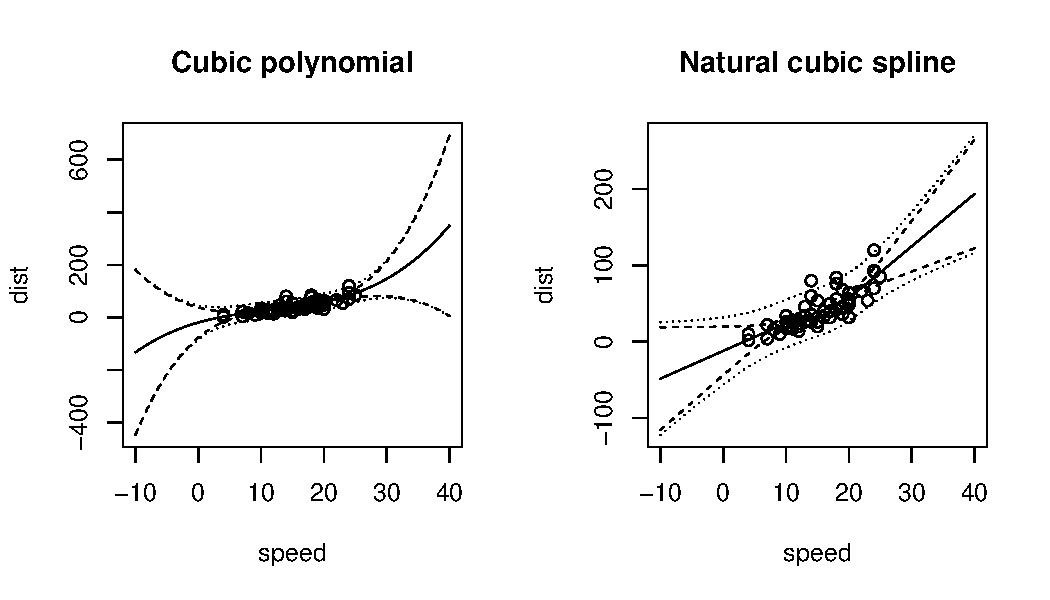
\includegraphics[width=\maxwidth]{figure/example-cars-plotFit} 

\end{knitrout}


\section{The \code{calibrate} function}
The most basic calibration problem, the one often encountered in more advanced regression texts, is the simple linear calibration problem for which
\begin{align*}
  \mathcal{Y}_i &= \beta_0 + \beta_1 x_i + \epsilon_i, \quad \epsilon_i \stackrel{iid}{\sim} \mathcal{N}\left(0, \sigma_\epsilon^2\right), \quad i = 1, \dotsc, n, \\
  \mathcal{Y}_{0j} &= \beta_0 + \beta_1 x_0 + \epsilon_{0j}, \quad \epsilon_{0j} \stackrel{iid}{\sim} \mathcal{N}\left(0, \sigma_\epsilon^2\right), \quad j = 1, \dotsc, m.
\end{align*}
For example, consider the arsenic data introduced in Section~\ref{sec:example_arsenic}. The following snippet of code obtains a 95\% inversion interval and 95\% Wald-based interval for the unknown $x_0$ corresponding to $y_0 = 3$ based on Equations~\eqref{eqn:x0_ci_inv} and \eqref{eqn:x0_ci_wald}, respectively:

\begin{knitrout}
\definecolor{shadecolor}{rgb}{0.969, 0.969, 0.969}\color{fgcolor}\begin{kframe}
\begin{alltt}
\hlkwd{calibrate}\hlstd{(arsenic.lm,} \hlkwc{y0} \hlstd{=} \hlnum{3}\hlstd{,} \hlkwc{interval} \hlstd{=} \hlstr{"inversion"}\hlstd{)}
\end{alltt}
\begin{verbatim}
## estimate    lower    upper 
##    2.931    2.537    3.325
\end{verbatim}
\begin{alltt}
\hlkwd{calibrate}\hlstd{(arsenic.lm,} \hlkwc{y0} \hlstd{=} \hlnum{3}\hlstd{,} \hlkwc{interval} \hlstd{=} \hlstr{"Wald"}\hlstd{)}
\end{alltt}
\begin{verbatim}
## estimate    lower    upper       se 
##   2.9314   2.5374   3.3255   0.1929
\end{verbatim}
\end{kframe}
\end{knitrout}


\noindent If instead we were interested in the unknown $x_0$ corresponding to a fixed mean response of $\mu_0 = 3$ (i.e., a regulation problem) we would instead use

\begin{knitrout}
\definecolor{shadecolor}{rgb}{0.969, 0.969, 0.969}\color{fgcolor}\begin{kframe}
\begin{alltt}
\hlkwd{calibrate}\hlstd{(arsenic.lm,} \hlkwc{y0} \hlstd{=} \hlnum{3}\hlstd{,} \hlkwc{interval} \hlstd{=} \hlstr{"inversion"}\hlstd{,}
    \hlkwc{mean.response} \hlstd{=} \hlnum{TRUE}\hlstd{)}
\end{alltt}
\begin{verbatim}
## estimate    lower    upper 
##    2.931    2.860    3.002
\end{verbatim}
\end{kframe}
\end{knitrout}


\section{The \code{invest} function}
In this section, we describe the more general function, \code{invest}, which can be used for more complex univariate calibration problems such as polynomial and nonlinear calibration.

For the quadratic linear model in the whiskey age example of Section\ref{sec:whiskey}, we used the following code to obtain a 95\% inversion interval for the unknown age corresponding to sample with a known proof of $108$:

\begin{knitrout}
\definecolor{shadecolor}{rgb}{0.969, 0.969, 0.969}\color{fgcolor}\begin{kframe}
\begin{alltt}
\hlstd{whiskey} \hlkwb{<-} \hlkwd{data.frame}\hlstd{(}\hlkwc{age} \hlstd{=} \hlkwd{c}\hlstd{(}\hlnum{0}\hlstd{,} \hlnum{0.5}\hlstd{,} \hlnum{1}\hlstd{,} \hlnum{2}\hlstd{,} \hlnum{3}\hlstd{,} \hlnum{4}\hlstd{,} \hlnum{5}\hlstd{,}
    \hlnum{6}\hlstd{,} \hlnum{7}\hlstd{,} \hlnum{8}\hlstd{),} \hlkwc{proof} \hlstd{=} \hlkwd{c}\hlstd{(}\hlnum{104.6}\hlstd{,} \hlnum{104.1}\hlstd{,} \hlnum{104.4}\hlstd{,} \hlnum{105}\hlstd{,} \hlnum{106}\hlstd{,}
    \hlnum{106.8}\hlstd{,} \hlnum{107.7}\hlstd{,} \hlnum{108.7}\hlstd{,} \hlnum{110.6}\hlstd{,} \hlnum{112.1}\hlstd{))}
\hlstd{whiskey.lm} \hlkwb{<-} \hlkwd{lm}\hlstd{(proof} \hlopt{~} \hlstd{age} \hlopt{+} \hlkwd{I}\hlstd{(age}\hlopt{^}\hlnum{2}\hlstd{),} \hlkwc{data} \hlstd{= whiskey)}
\hlkwd{invest}\hlstd{(whiskey.lm,} \hlkwc{y0} \hlstd{=} \hlnum{108}\hlstd{)}
\end{alltt}
\begin{verbatim}
## estimate    lower    upper 
##    5.233    4.678    5.735
\end{verbatim}
\end{kframe}
\end{knitrout}


As for a nonlinear regression example, we consider the nasturtium example of Section~\ref{sec:nasturtium}. The following snippet of code fits the log-logistic regression function
\begin{equation*}
  \mu(x; \beta_1, \beta_2, \beta_3) = \left\{ \begin{array}{l l}
                                              \beta_1, &\quad x = 0 \\
                                              \beta_1 / \left[1 + \exp\left\{\beta_2 + \beta_3\ln(x)\right\}\right], &\quad x > 0
                                            \end{array} \right..
\end{equation*}
to the data and obtains both a 95\% inversion interval and 95\% Wald-based interval for the unknown concentration corresponding to the three unknowns $309$, $296$, and $419$:

\begin{knitrout}
\definecolor{shadecolor}{rgb}{0.969, 0.969, 0.969}\color{fgcolor}\begin{kframe}
\begin{alltt}
\hlstd{nas.nls} \hlkwb{<-} \hlkwd{nls}\hlstd{(weight} \hlopt{~} \hlkwd{ifelse}\hlstd{(conc} \hlopt{==} \hlnum{0}\hlstd{, theta1, theta1}\hlopt{/}\hlstd{(}\hlnum{1} \hlopt{+}
    \hlkwd{exp}\hlstd{(theta2} \hlopt{+} \hlstd{theta3} \hlopt{*} \hlkwd{log}\hlstd{(conc)))),} \hlkwc{data} \hlstd{= nasturtium,}
    \hlkwc{start} \hlstd{=} \hlkwd{list}\hlstd{(}\hlkwc{theta1} \hlstd{=} \hlnum{1000}\hlstd{,} \hlkwc{theta2} \hlstd{=} \hlnum{0}\hlstd{,} \hlkwc{theta3} \hlstd{=} \hlnum{1}\hlstd{))}
\hlkwd{invest}\hlstd{(nas.nls,} \hlkwc{y0} \hlstd{=} \hlkwd{c}\hlstd{(}\hlnum{309}\hlstd{,} \hlnum{296}\hlstd{,} \hlnum{419}\hlstd{),} \hlkwc{interval} \hlstd{=} \hlstr{"inversion"}\hlstd{)}
\end{alltt}
\begin{verbatim}
## estimate    lower    upper 
##    2.264    1.772    2.969
\end{verbatim}
\begin{alltt}
\hlkwd{invest}\hlstd{(nas.nls,} \hlkwc{y0} \hlstd{=} \hlkwd{c}\hlstd{(}\hlnum{309}\hlstd{,} \hlnum{296}\hlstd{,} \hlnum{419}\hlstd{),} \hlkwc{interval} \hlstd{=} \hlstr{"Wald"}\hlstd{)}
\end{alltt}
\begin{verbatim}
## estimate    lower    upper       se 
##   2.2639   1.6889   2.8388   0.2847
\end{verbatim}
\end{kframe}
\end{knitrout}


Bootstrap approaches to obtaining calibration intervals are currently not available in the \pkg{investr} package, however, a future release is likely to contain some bootstrap functionality. Until such time, the well-known \pkg{boot} package can be used to obtain the bootstrap calibration intervals described in Chapter~\ref{chap:lit-review}. The \code{bootMer} function from the \code{R} package \pkg{lme4} ($\ge 1.0-5$) can be used to obtain the parametric bootstrap calibration intervals discussed in Chapter~\ref{chp:cal-dependent}.


% The \references command should be used to insert the list of references.
% Assuming one is using BibTeX, this should contain both a \bibliographystyle
% and a \bibliography command referencing a separate bibliography file.

\references{
  \bibliographystyle{abbrvnat}
  \bibliography{References}
}

\end{document}

